\documentclass[12pt,a4paper]{book}
\usepackage[utf8]{inputenc}
\usepackage[a4paper,bindingoffset=0.2in,%
            left=1in,right=1in,top=1in,bottom=1in,%
            footskip=.25in]{geometry}
\usepackage{amsmath}
\usepackage{amsfonts}
\usepackage{amssymb}
\usepackage{graphicx}
\usepackage{supertabular}
\usepackage{tabto}
\usepackage[section]{placeins}
\usepackage[toc,page]{appendix}
\newcommand{\namesigdate}[2][5cm]{%
  \begin{tabular}{@{}p{#1}@{}}
    #2 \\[2\normalbaselineskip] \hrule \\[0pt]
    {\small \textit{Signature}} \\[2\normalbaselineskip] \hrule \\[0pt]
    {\small \textit{Date}}
  \end{tabular}
}
\pagestyle{plain}
\linespread{1.5}
\author{Thomas C.K. Fuller}
\title{Experimental Celestial Navigation Prototype for Computer Vision Based Nautical Sight Reduction}
\begin{document}
\frontmatter
\begin{titlepage}
	\centering
	{\scshape\large \textbf{EXPERIMENTAL CELESTIAL NAVIGATION PROTOTYPE FOR COMPUTER VISION BASED NAUTICAL SIGHT REDUCTION}\par}
	\vspace{1.75cm}
	{\scshape\normalsize BY\par}
	\vspace{2.25cm}
	{\normalsize THOMAS C.K. FULLER\par}
	{\normalsize B.S. in Electromechanical Engineering, Wentworth Institute of Technology, Boston, 2013\par}
	
	\vspace{2cm}
	{\normalsize THESIS\par}
	\vspace{2.5cm}
	{\normalsize Submitted to the University of New Hampshire\par}
	{\normalsize In Partial Fulfillment of the Requirements for the Degree of\par}
	{\normalsize Master of Science\par}
	{\normalsize in\par}
	{\normalsize Mechanical Engineering\par}


	\vfill

% Bottom of the page
	{\normalsize September, 2016\par}
\end{titlepage}
%\maketitle
%\frontmatter
\begin{center}
%EXPERIMENTAL CELESTIAL NAVIGATION PROTOTYPE FOR COMPUTER VISION BASED NAUTICAL SIGHT REDUCTION

\vspace{1cm}
%{\normalsize BY}\\
%\vspace{1cm}
%{\normalsize THOMAS C.K. FULLER}
\end{center}
\vspace{2cm}
This thesis has been examined and approved in partial fulfillment of the requirements for the degree of Master of Science in Mechanically Engineering by
\vspace{2cm}
\\
\hspace*{3cm}
\begin{supertabular}{p{12cm}}
%      \begin{tabular}{l}
         %\vspace{10mm}\\
%      \hline
         {Thesis Director, Dr. May-Win L. Thein},\\
         \small{Associate Professor of Mechanical Engineering and Ocean Engineering} \\
         \vspace{2.5mm} \\
%      \hline
         {Dr. Barry Fussell},\\
         \small{Professor of Mechanical Engineering}
         \\
         \vspace{2.5mm}\\
%      \hline
         {Dr. Michael Carter},\\
         \small{Associate Professor of Electrical \& Computer Engineering} \\
        % \vspace{5mm}\\
     % \hline
        % \textbf{Pete P. Peterson},
        % \small{Professor of Ocean Engineering and Earth Sciences} %\\
        % \vspace{5mm}\\
      %\hline
        % \textbf{Rob Robertson},
         %\small{Professor of Mechanical Engineering and Ocean Engineering} \\
        % \vspace{5mm}\\
      %\hline
        % \textbf{Frank Frankelson},
        % \small{Professor of Civil Engineering and Ocean Engineering} \\
         \vspace{6mm}\\
%    \end{tabular}
    \end{supertabular}

 \hspace*{6cm}   \begin{tabular*}{2in}{l}
%      \hline
        On 27-May-2016
        \vspace{6mm}

    \end{tabular*}
        \\
        Original approval signatures are on file with the University of New Hampshire Graduate School.



%\vspace{
\newpage
\begin{center}
\section*{Dedication}
\vspace{8cm}
Dedicated to Craig Curtis, role model and friend.
\clearpage
\end{center}
\section*{Acknowledgments}
This research was made possible by the contributions of many people. First thanks to Prof. May-Win Thein, for advising this project since August 2013 and affording me many opportunities over my time at UNH.  Thank you to Prof. Barry Fussell and Prof. Michael Carter for serving on the thesis committee. \\ \\
Christopher Hashem and I have been studying together for the last eight years of undergraduate and graduate school.  That's important for me to put here.  \\\\
To Mike Johnson and Shuai Chen, this work wouldn't have been possible without your contributions in the optimization techniques and the design of the experimental setup.\\\\
This research was greatly aided through the many conversations I had with William Nitsch about image processing and machine learning. \\\\
Thank you to the Mechanical Engineering Department for supporting me through assistantship during my time at UNH.\\\\
Lastly I'd like to thank my mom, Mimi Wong and my dad, John Fuller for encouraging me to set and reach high goals such as this one.

\tableofcontents
\listoffigures
\listoftables
\newpage
\break
\begin{center}
\section*{ABSTRACT}

EXPERIMENTAL CELESTIAL NAVIGATION PROTOTYPE FOR COMPUTER VISION BASED NAUTICAL SIGHT REDUCTION\break
by\break
Thomas C.K. Fuller\break
University of New Hampshire, September 2016
\end{center}
This thesis presents the development and analysis of an experimental platform for celestial navigation using the Directly Computed Nautical Sight Reduction Algorithm.  The goal is to obtain an estimate of latitude and longitude using an image of the stars and measurements from an IMU as an input.  Analytical simulation results indicate that the presented method is viable for navigation for three different observational formats and a wide range of camera pointing directions.  Experimental development is presented including cost function analysis for minimizing the error in the position estimate.  The results of the optimization were that an error of $0.0585^{\circ}$, approximately 3 nautical miles, was achieved.  The presented device is also compared to other established methods of celestial navigation.
%This study presents an experimental device capable of estimating static position (latitude, longitude) using an image of the stars.  The presented star camera takes an optical light image of the stars and sensor measurements from a 3-axis IMU to determine the local orientation of the image.  The image is processed by the Astrometry.net blind astrometric calibration software to determine the names and pixel locations of three stars in the image.  These pixel locations are processed by a program that assigns the value of IMU pitch and roll to the center pixel of the image in order to create viable measurement of the altitude of the stars.  These altitude angles are fed as inputs to a software version of the Directly Computed Nautical Sight Reduction Algorithm to determine an estimate of the position.  
%This thesis examines a number of other methods of celestial navigation and describes the motivation behind the selection of the Nautical Sight Reduction Algorithm.
%Simulations of the Nautical Sight Reduction method are presented to determine the theoretical viability of the algorithm.  These simulations also examine the effects of uniform and non-uniform noise and bias. Simulations are also used to determine the approximate expected error of the star camera given the equipment selected for use in the experimental set up.
%Experimental results show that without any modifications, the star camera is locating a position based on an altitude measurement of stars in an image.  A cost function is developed to minimize the error and an optimization method was applied that reduced the position estimate error to approximately $0.0586^{\circ}$. This angular error suggests that an error circle of approximately 3 nautical miles is possible.   
%The results of the simulations and experiments are compared to other established methods of celestial navigation.  Results of this analysis show that the presented method is capable of improved estimates over the Compass Star Tracker (Attitude Matrix Formulated Method) and is also comparable to other self contained methods of celestial navigation after optimization.  
\mainmatter
\chapter{Introduction}
\section{Methods of Celestial Navigation}
Lander and rover type vehicles have been a primary source of scientific insight when exploring the surface of another planet. There has been a trend of surface exploration missions from intentional hard impact, to soft lander, and finally to the modern rover.  Each of these exploration techniques has improved scientific output of the surface exploring apparatus.  The first extraterrestrial landing was performed by \textit{Luna 2} \cite{b:luna}.  This device was intentionally impacted on the surface of the moon.  While it was able to determine some interesting properties of the magnetic field and Van Allen belt, due to the strong impact force of the probe, very little information was revealed about target surface, that of the moon.  Soft landing, being a requirement for manned lunar landing, was an area of active research during the 1960s and was first achieved on the Moon by \textit{Surveyor 1} on 30-May-1966.  This probe delivered important scientific results including data on bearing strength, temperatures, and radar reflectivity of the moon \cite{b:surveyor}.  It can be seen from Fig.~\ref{f:datarates} that data transmission rates for space systems will only increase in the future.  

\begin{figure}[h!]
\centering
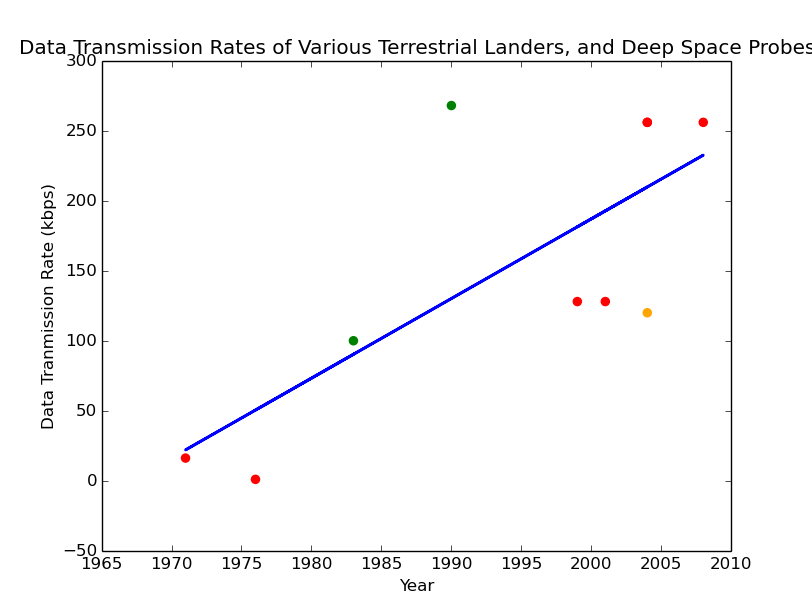
\includegraphics[scale=0.60]{datarates.png}
\caption{Data Transmission Rates for Various Extraterrestrial Probes. Line of Best fit included.  Different colors indicate different destination planets \cite{b:mpl},\cite{b:messenger},\cite{b:mitchell}}
\label{f:datarates}
\end{figure}

This greater data rate necessitates better functionality from extraterrestrial mobility solutions.  Navigational capability has ceased to be a fancy, non-required feature.  It is greatly increasing the scientific yield of exploratory rovers.  Improvement of such techniques will only serve to increase the amount of science yield.  

Different methods of extraterrestrial navigation have been performed.  Due to the prohibitive nature of implementing a GPS constellation in orbit around interesting celestial bodies, these methods all have some celestial navigation component.  The methods surveyed here are the Deep Space Network, Phobos Transit Method, Attitude Matrix Formulated Method, Modified Attitude Matrix Formulated Method, and the Nautical Sight Reduction Method.
\subsection*{Deep Space Network}
The Deep Space Network is a comprehensive communications network used for communication with current deep space probes.  The Deep Space Network uses light from a quasar in conjunction with three ground stations located in Barstow, California, Madrid, Spain, and Canberra, Australia \cite{b:dsn}.  Deep Space Network is extremely accurate, leading to position error circles between 5 and 10 meters for certain applications \cite{b:msla}.  This level of accuracy is possible over a widespread variety of applications from surface exploration to deep space flybys.  The primary limitations of Deep Space Network are that it has a geometric weakness in the southern declinations and that it requires a precisely timed interaction between the ground station, a quasar, and the vehicle it is implemented on \cite{b:dor}. The device presented in this research is unlikely to achieve this accuracy on the surface of another planet.  It is possible to implement an experimentally feasible, self-contained celestial navigation device which does not require complicated infrastructure.  
\subsection*{Phobos Transit Method}
The Phobos Transit Method is a method that relies on visual observations of the martian moon Phobos for navigating the Martian surface.  The Phobos transit method has a theoretical accuracy of approximately 5000m and it may be possible to reduce that error to approximately 2000m.  It is theoretically possible that by using detailed models of interesting celestial bodies, with the intention of more accurately estimating sidereal time, and therefore local hour angle, that this method could be applicable to any celestial body with a sattelite whose properties of motion are known.   As of yet, this method has not been verified experimentally by rovers on the surface of Mars   \cite{b:phobos}.  Further analysis on on the calculation of sidereal time, nutation, precession, and abberation effects for Martian celestial navigation was examined by Malay et. al  \cite{b:mars}.  It should also be noted that this method has great potential for self containment, and would be possible to implement without a supporting satellite or communications network. 
\subsection*{Attitude Matrix Formulated Method}
The attitude matrix formulated method was first developed by Samaan et. al \cite{b:gps}.  This self-contained method uses attitude matrices as well as a star imaging software based on the Pyramid-LISA algorithm. This method was brought to experimental life as the Compass Star Tracker.  The Compass Star Tracker was relatively successful as a proof of concept device.  The attitude matrix formulated method obtained an experimental accuracy of 61.23 miles, or 98.54km \cite{b:swanzy}.  The primary disadvantage of this method is that the camera optical axis must be aligned with the zenith to ensure maximum accuracy.  Attempts to reduce or eliminate this zenith orientation requirement did not seem to be successful.   Chapter 2 will discuss this method in much greater detail.  
\subsection*{Modified Attitude Matrix Formulated Method}
The modified attitude matrix formulated method was developed by Thein et al.  It is essentially the attitude matrix formulated method, with an emphasis on misalignment and sensor implementation.  This allowed interesting analytical calculations of the accuracy to be computed.  It was found that for an accuracy of 50m in this implementation, the combined errors of all orthogonal misalignment needed to be less than 5.93 arcseconds \c3ite{b:quinn}.  One major concern in the past research is experimental verification of this method.  Experimental results were found using a backtracking method \cite{b:perkinsthesis}.  This method uses the current position as an input, and is used to show that a valid star tracker and inertial measurement unit rotations could be obtained.  Correct celestial navigation must occur in reverse of this backtracking process.  The position must be the output, and an observation of the celestial bodies must be an input.
\subsection*{Nautical Sight Reduction Method}
The method of celestial navigation used by this thesis is called Nautical Sight Reduction, detailed in the Nautical Almanac \cite{b:naut}.  The presented implementation uses a computer vision technique to observe three or more stars.  The primary concept is that an imaginary line could be drawn from the star through the center of the Earth. The point where that line intersects the surface of the earth is called the ground position.  Then, if the angle from the horizon to the celestial body could be measured, a locus of points where that angle is constant could be drawn.  This locus of points is called a circle of position. The center of the circle of position is the ground position of the observed star.  Three or more circles of position are intersected to determine an estimate of the observer's position.  This concept is illustrated in Fig.~\ref{f:circles}

\begin{figure}[h!]
\centering
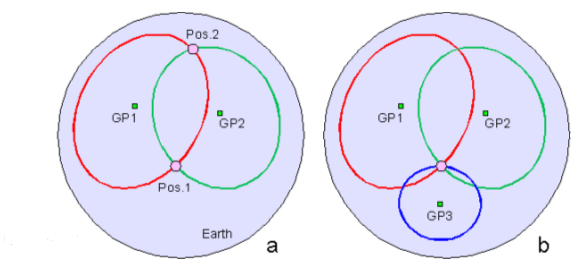
\includegraphics[scale=0.35]{circles.png}
\caption{Diagram of Nautical Sight Reduction Method \cite{b:celnavde}}
\label{f:circles}
\end{figure}
\section{Research on Extra-Terrestrial Surface Navigation}
One goal of the University of New Hampshire Advanced Controls Laboratory is a complete Guidance, Navigation, and Control solution for navigation on celestial bodies. This solution is represented by the block diagram of Fig.~\ref{f:blocks}
\begin{figure}[h!]
\centering
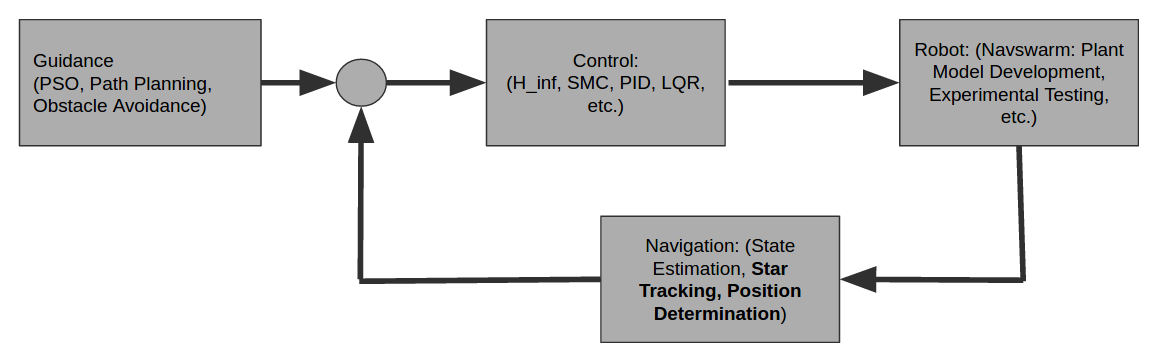
\includegraphics[scale=0.35]{blocks.png}
\caption{Complete Guidance, Navigation, and Control Solution for Extraterrestrial Surface Navigation.  The material discussed in this thesis are bolded in the feedback block. \cite{b:fuller}}
\label{f:blocks}
\end{figure}
On the part of Guidance, work performed by Johnson and Thein examined the use of the Particle Swarm Algorithm, obstacle avoidance, and path planning \cite{b:johnson}.  Particle Swarm is a distributed optimization algorithm being used in a novel way; It optimizing its cost function will be used for extraction of natural resources.  The additional features will be to this system, because they allow generic rovers, known as mobility solutions to traverse dangerous paths. One important part of this work is the senior project team ET-Navswarm.  The Navswarm is a fleet of autonomous rovers on which the guidance, navigation, and controls will be experimentally verified.

On the part of Controls, work performed by Underwood and Thein used a differential-drive mobility solution with the same plant model as the Navswarm rover \cite{b:underwood}.  Their study surveyed the use various control algorithms for vehicle motion.  These controllers included Proportional Integral Differential (PID) control, Linear Quadratic Regulator (LQR) control, $H_{\infty}$ Optimal Control, Fuzzy-LQR, and Sliding Mode Control (SMC).  These controllers evaulated on the criteria of efficiency, accuracy, speed of response, controller effort, actuator effort, steady state error, robustness to noise and disturbances, computational effort, and ease of implementation.  This work concluded that given enough computational power, the optimal $H_{\infty}$ controller would be the controller of choice for the differential drive mobility solution.  If computational power is a scarce resource for the Navswarm rover, then SMC is the recommended controller, due to its performance compared to its ease of implementation. It is worth noting that of the examined controllers, SMC had the highest amount of control effort.   

On the part of Navigation, work done by Perkins and Thein examined the use of a matrix formulated algorithm for use in celestial navigation.  This is a modification of an algorithm originally proposed by Samaan et. al \cite{b:gps}.  Perkins and Thein examined the use of several feedback estimation techniques for the mobility solution.  These estimators included Extended Kalman Filter (EKF), Sliding Mode Observer (SMO), and $H_{\infty}$ Observer.  For ease of implementation these observers were simulated on the mobility solution with a PID controller.  Perkins concluded, similarly to Underwood, that the $H_{\infty}$ optimal observer method drove the state error closest to zero, and that SMO had the least computational time.  Monte Carlo analysis was performed to study the position based error.  In that study it was found that a angular error in longitude was a function of latitude, and that the error decreased as the estimate was closer to the poles.  The was an expected result because lines of longitude converge at the pole.

\section{Thesis Contributions}
The primary objective of this thesis is to provide the theory and proof-of-concept experimental platform for a self-contained device that can use an image of the stars and output meaningful position data. This would eliminate the need for the backtracking method performed by Perkins and Underwood.  A secondary objective is to demonstrate the ability of this device to use a wide range of zenith angles.  This would be an improvement over the Compass Star Tracker, which needed to be as close to zenith oriented as possible \cite{b:swanzy}.  The tertiary objective are to provide some analysis on the performance of the individual sensors and overall accuracy of the device. This work serves as the first step to achieving an experimental platform for dynamic control of an extraterrestrial robotic mobility solution using celestial navigation.  
\section{Thesis Outline}
\textbf{Chapter 1: Introduction} Introduces the problem statement, background research, and the thesis outline.
\\
\textbf{Chapter 2:  Celestial Navigation Algorithms}  This chapter discusses the matrix formulated celestial navigation algorithm.  Its properties, and the decision to change algorithms are discussed.  The new algorithm is proposed. The method for locating the stars in an image is the Blind Astrometric Calibration Method.  The method for using the star locations to determine location is called the Sight Reduction method.  These two methods are discussed separately, then their integration into one navigational algorithm is proposed.  
\\
\textbf{Chapter 3:  Simulation of Nautical Sight Reduction Algorithm}  Simulations are presented in order to determine the validity of the new algorithm.  Tests performed include observational format, accuracy, and uncertainty and error analysis.
\\
\textbf{Chapter 4:  Experimental Design and Verification}  The developed experimental solution is discussed along with experimental results and analysis on accuracy, uncertainty, and sensor communication.  A generic optimization method of calibrating unknown pitch and roll misalignment is proposed and preliminary results are presented.
\\
\textbf{Chapter 5: Discussion} This section discusses the results of the theoretical derivations, the simulations, and the experiments presented in the previous chapters.  This section discusses present successes and failures and makes suggestions on future works.
\\
\textbf{Chapter 6:  Conclusions}  The thesis conclusions are made, relating the objectives set forth in Chapter 1 to the progress that was made throughout the thesis.

\chapter{Celestial Navigation Algorithms}
In this chapter, three algorithms are discussed in detail.  The first one is the matrix formulated algorithm developed by  et. al \cite{b:gps}.  The second is a modified matrix formulated method developed by Thein et. al \cite{b:quinn}.  The third is the presented algorithm of this thesis, which is based on Nautical Sight Reduction.
\section{Attitude Matrix Formulated Method (Compass Star Tracker)}
The Attitude Matrix Formulated method, which in this work will also be referred to as the Compass Star Tracker, determines the relative attitudes of four different reference frames. The references frames will be denoted by \textbf{$A^{X/Y}$} to indicate that this matrix rotates the attitude from X to Y coordinate frames.   

Four coordinate frames are defined in this research are identical to those defined in the Compass Star Tracker.  They are denoted by the following letters. B is the body or camera reference frame.  I is the inertial, geocentric reference frame.  G is the Greenwich reference frame.  and L is the local reference frame.  

\begin{figure}[h!]
\centering
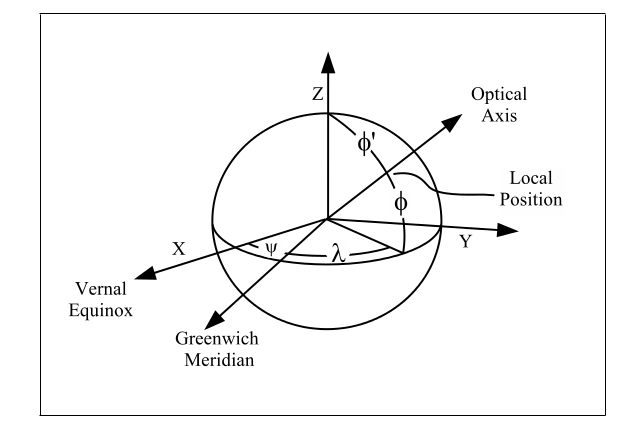
\includegraphics[scale=0.35]{inertial.png}
\caption{Inertial Reference Frame for Celestial Navigation}
\label{f:inertial}
\end{figure}

\begin{figure}[h!]
\centering
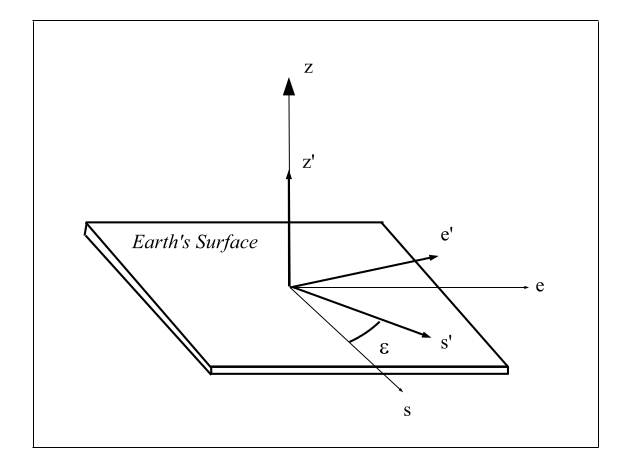
\includegraphics[scale=0.35]{local.png}
\caption{Local Reference Frame for Celestial Navigation}
\label{f:local}
\end{figure}

The notation is also largely the same as with the Compass Star Tracker, 

\begin{itemize}
\item $\psi(t)$ is the angle between the vernal equinox and the Greenwich Meridian.
\item $\lambda$ is the longitude
\item $\phi$ is the latitude
\item $\phi^{'}$ is the compliment of latitude $\phi$.
\item $\vec{oa}$ is the pointing direction of the camera.  In Fig.~\ref{f:local}, this is denoted as $z^{'}$
\end{itemize}

In the original attitude matrix formulation (Compass Star Tracker), the camera optical axis was assumed to be aligned with the zenith direction.  This work provides some experimental confirmation that that is not necessary.  Given such a zenith requirement, the attitude transformation between the body and local coordinate frames are given as

\begin{equation}
A^{B/L} = \begin{bmatrix}
cos(\epsilon) & sin(\epsilon) & 0\\
-sin(\epsilon) & cos(\epsilon) & 0 \\
0 & 0 & 1
\end{bmatrix}
\label{e:compass1}
\end{equation}

Eq.(\ref{e:compass1}) is where the CST gets the ``Compass" part of its name.  Later on we will see that the derivation of $A^{B/L}$, called $\Gamma$ in the modified attitude matrix formulation, so simple if the CST is at a non-zenith pointing orientation.  Given a time invariant system, the rest of the attitude matrices are straightforward to derive.  The attitude transformation between the local reference frame and the Greenwich frame are given by

\begin{equation}
A^{L/G} = R_{2}(\phi^{'})R_{3}(\lambda) = \begin{bmatrix}
cos(\phi^{'}) & 0 & -sin(\phi^{'})\\
0 & 1 & 0 \\
sin(\phi^{'}) & 0 & cos(\phi^{'})
\end{bmatrix}\begin{bmatrix}
cos(\lambda) & sin(\lambda) & 0\\
-sin(\lambda) & cos(\lambda) & 0\\
0 & 0 & 1
\end{bmatrix}
\end{equation}

\begin{equation}
A^{L/G} = \begin{bmatrix}
cos(\phi^{'})cos(\lambda) & cos(\phi^{'})sin(\lambda ) & -sin(\lambda)\\
-sin(\lambda) & cos(\lambda) & 0\\
sin(\phi^{'})cos(\lambda) & sin(\phi^{'})sin(\lambda) & cos(\phi^{'})
\end{bmatrix}
\end{equation}

The next attitude that is transformed about is from Greenwich to Inertial Frame.  To do this many interesting factors are considered.  These exact factors are given in a later section of this chapter.  In a simplified version of this equation, the three unknown variables for position determination are $\phi$, $\lambda$, and $\epsilon$.   These parameters can be solved as follows.
\begin{equation}\begin{bmatrix}
A^{B/L}A^{L/G} = A^{B/I}A^{I/G} = A
\end{bmatrix}
\end{equation}

The product of $A^{B/I}$ and $A^{G/I}$ is known because $A^{B/I}$ is determined from from the star tracking and attitude determination algorithms.  All the unknown parameters are contained in the left side of the given equation.  This equation can be given as

\begin{equation}
A^{B/L}A^{L/G} = \begin{bmatrix}
cos(\epsilon) & sin(\epsilon) & 0\\
-sin(\epsilon) & cos(\epsilon) & 0 \\
0 & 0 & 1
\end{bmatrix}\begin{bmatrix}
cos(\phi^{'})cos(\lambda) & cos(\phi^{'})sin(\lambda ) & -sin(\lambda)\\
-sin(\lambda) & cos(\lambda) & 0\\
sin(\phi^{'})cos(\lambda) & sin(\phi^{'})sin(\lambda) & cos(\phi^{'})
\end{bmatrix}
\end{equation}

{\scriptsize\begin{equation}
A^{B/L}A^{L/G} = \begin{bmatrix}
cos(\epsilon)cos(\phi^{'})cos(\lambda)-sin(\epsilon)sin(\lambda) & cos(\epsilon)cos(\phi^{'})sin(\lambda)+sin(\epsilon) & -cos(\epsilon)sin(\phi^{'})\\
-sin(\epsilon)cos(\phi^{'})cos(\lambda)-cos(\epsilon)sin(\lambda) & -sin(\epsilon)cos(\phi^{'})sin(\lambda)+cos(\epsilon)cos(\lambda) & sin(\epsilon)sin(\phi^{'})\\
sin(\phi^{'})cos(\lambda) & sin(\phi^{'})sin(\lambda) & cos(\phi^{'})
\end{bmatrix}
\end{equation}}

From the above matrix, called $\Phi$ in some literature, $\lambda$, $\epsilon$, and $\phi$ can be obtained.  
\begin{equation}
\lambda = atan2[A(3,2), A(3,1)]
\end{equation}

\begin{equation}
\epsilon = atan2[A(2,3), -A(1,3)]
\end{equation}

Where the atan2 function deals with ambiguities related to what quadrant its arguments are in.  It is given as
\begin{equation}
\operatorname{atan2}(y,x) =
\begin{cases}
\arctan(\frac y x) &\text{if } x > 0, \\
\arctan(\frac y x) + \pi &\text{if } x < 0 \text{ and } y \ge 0, \\
\arctan(\frac y x) - \pi &\text{if } x < 0 \text{ and } y < 0, \\
+\frac{\pi}{2} &\text{if } x = 0 \text{ and } y > 0, \\
-\frac{\pi}{2} &\text{if } x = 0 \text{ and } y < 0, \\
\text{undefined} &\text{if } x = 0 \text{ and } y = 0.
\end{cases}
\end{equation}
The atan2 function takes the arctangent and avoids issues based on the quadrant x and y are in.

The latitude $\phi^{'}$ is given as

\begin{equation}
	\phi = 90 - \frac{A(3,2)}{sin(\lambda)}
\end{equation}
\subsection*{Modified Attitude Matrix Formulated Method}
The modified attitude matrix is the same general concept of changing attitudes, and shown below in Eq~(\ref{e:unhalg}).  

\small{\begin{equation}
[H(\epsilon)]^{Down}_{NED}[U]^{NED}_{ENU}[LL(\lambda,\phi)]^{ENU}_{SD} = [\Phi] = [\Gamma]^{Down}_{A}[M_{A}]^{A}_{Body}([\Omega]^{SD}_{Inertial}[\Delta]^{Inertial}_{C}[M_{C}]^{C}_{Body})^{T}
\label{e:unhalg}
\end{equation}}
Eq.(\ref{e:unhalg}) performs the same rotation matrices as the Compass Star Tracker algorithm.  The right hand side of this equation describes the accelerometer ($\Gamma$) matrix and the star tracker ($\Delta$) matrix. $M_{A}$ and $M_{C}$ are the respective misalignments.  $\Omega$ is the planetary (lunar) model.  This allows simple analysis of misalignments between the accelerometer and body frame in $M_{A}$, and the star tracker  and inertial frame in $M_{C}$ \cite{b:quinn}.  In the next section, we will see some analysis of the $\Gamma$ and $\Delta$ matrices which led to the selection of the current algorithm.  The first is an analysis of the modified attitude matrix version of $\Gamma$ and presents a more efficient, correct method by which the body to local coordinate transformation can be performed.

\section{Star Tracker Matrix, $\Delta$ for Modified Attitude Matrix Method}
The modified attitude matrix formulation showed that the $\Delta$ matrix begins with the star tracker quaternion.  Note that the variables $\theta$ and $\beta_{i}$ are generic quaternion components, for use in the general case.

\begin{equation}
StarTracker_{measured} = 
\begin{bmatrix}
q_{1}\\
q_{2}\\
q_{3}\\
q_{0}
\end{bmatrix} = 
\begin{bmatrix}
sin(\frac{\theta}{2})cos(\beta_{x})\\
sin(\frac{\theta}{2})cos(\beta_{y})\\
sin(\frac{\theta}{2})cos(\beta_{z})\\
cos(\frac{\theta}{2})
\end{bmatrix}
\end{equation}
The quaternion values were assembled into a 3x3 matrix with the following format
\begin{equation}
M = \begin{bmatrix}
Q_{1} & Q_{2} & Q_{3}
\end{bmatrix}
\end{equation}
where,
\begin{equation}
Q_{1} = \begin{bmatrix}
q_{1}^{2} - q_{2}^{2} - q_{3}^{2} + q_{0}^{2}\\
2(q_{1}q_{2} - q_{3}q_{4})\\
2(q_{1}q_{2} + q_{3}q_{4})
\end{bmatrix}
\end{equation}

\begin{equation}
Q_{2} = \begin{bmatrix}
2(q_{1}q_{2} + q_{3}q_{4})\\
-q_{1}^{2} - q_{2}^{2} - q_{3}^{2} + q_{4}^{2}\\
2(q_{1}q_{2} - q_{3}q_{4})
\end{bmatrix}
\end{equation}

\begin{equation}
Q_{1} = \begin{bmatrix}
2(q_{1}q_{2} - q_{3}q_{4})\\
2(q_{1}q_{2} + q_{3}q_{4})\\
-q_{1}^{2} - q_{2}^{2} + q_{3}^{2} + q_{4}^{2}
\end{bmatrix}
\end{equation}

The derivations of the modified attitude matrix formulated method did not provide a detailed relationship between an observation the stars and this quaternion/rotation matrix.  The original attitude matrix formulation used an algorithm called Pyramid-LISA \cite{b:pyramid}.  In the presented research, a similar method called the Blind Astrometric Method will be used to address that the star tracker measurement should obtained using an observation of the stars, as opposed to the backtracker method.

\section{Body to Local Rotation Matrix, $\Gamma$}
The accelerometer rotation matrix $\Gamma$ rotates from the body to local coordinate frames.  In some literature it is denoted as $A^{B/L}$.  Experimental implementation of this matrix is done using an accelerometer or other device that can measure roll ($\xi$) and pitch ($\psi$). Without certain mechanical restraints, the roll and pitch angles of the accelerometer are not related to the body frame by successive Euler angles. This is called non-orthogonal rotation. If this mechanical restraint was in place, or the matrices were orthogonal, then the $\Gamma$ matrix would be the product of the roll and pitch rotation matrices,

\begin{equation}
R2(\psi)R1(\xi) = 
\begin{bmatrix}
cos(\psi) & 0 & -sin(\psi)\\
0 & 1 & 0\\
sin(\psi) & 0 & cos(\psi)
\end{bmatrix}
\begin{bmatrix}
1 & 0 & 0\\
0 & cos(\xi) & sin(\xi)\\
0 & -sin(\xi) & cos(\xi)
\end{bmatrix}
\label{e:something}
\end{equation}

The Body frame corresponds directly to the optical axis, and the Local frame is corresponding to the position of the entire apparatus.  Using the rotation matrices from Eq.(\ref{e:something}), the camera optical axis and rover zenith direction are not required to be aligned.  Here, the two algorithms diverge in methods.  The UNH algorithm uses vector methods to determine the shortest arc between two points.  The algorithm developed by Texas A\&M uses a geometric method to relate the accelerometer readings.  

\subsection{Modified Attitude Matrix Method $\Gamma$ Matrix}
The modified attitude matrix method $\Gamma$ matrix is computed by the following general steps.  The output of the inclinometer (accelerometer) is expressed as a unit vector offset from the rover local downwards vector.  The accelerometer output is assumed to have the form of Eq.(\ref{e:accelerometerForm})

\begin{equation}
Acc_{measured} = \begin{bmatrix}
x\\
y\\
z
\end{bmatrix} = y\mathbf{i} + y\mathbf{j} + z\mathbf{k}
\label{e:accelerometerForm}
\end{equation}

The 3x3 $\Gamma$ matrix is then formulated column by column with the first column, corresponding to the x-axis being derived as follows.  

\textbf{Modified x-axis formulation:}
Let $\eta_{x}$ and $\theta_{1}$ represent the unnormalized pointing vector about the x-axis.  The rotation vector about the x axis is given as:

\begin{equation}
\eta^{'}_{x} = \mathbf{i} \times (x\mathbf{i} + y\mathbf{j} + z\mathbf{k}) = x\mathbf{k} - z\mathbf{j}
\end{equation}
Where $\times$ symbol represents the vector cross product. It is desired that this will be put into quaternion form, so normalizing the vector is required.  This gives
\begin{equation}
\eta_{x} = \frac{y\mathbf{k} - z\mathbf{j}}{\sqrt{y^{2}+z^{2}}}
\end{equation}
Then, using the vector dot product definition, the angle between the rover nadir vector and the measurement of the gravitational field can be found.
\begin{equation}
\mathbf{A}\cdot \mathbf{B} = (|\mathbf{A}|)(|\mathbf{B}|)cos(\theta)
\end{equation}
Leads to
\begin{equation}
\theta_{1} = cos^{-1}[\mathbf{i}\cdot \frac{x\mathbf{i}+y\mathbf{j}+z\mathbf{k}}{\sqrt{x^2 + y^2 + z^2}} = cos^{-1}\frac{x}{\sqrt{x^2 + y^2 + z^2}}
\end{equation}
This projection of the unit gravitational vector can be related to a quaternion, $q_{1}$ such that:
\begin{equation}
q_{1} = \begin{bmatrix}
sin(\frac{\theta_{1}}{2}) * 0\\
sin(\frac{\theta_{1}}{2}) * \frac{-z}{\sqrt{y^{2} + z^{2}}}\\
sin(\frac{\theta_{1}}{2}) * \frac{y}{\sqrt{y^{2} + z^{2}}}\\
cos(\frac{\theta_{1}}{2})
\end{bmatrix}
\end{equation}
Then, converting from quaternions to Euler angles, the first column of $\Gamma$ can be found as:
\begin{equation}
\Gamma_{1} = \begin{bmatrix}
x\\
\frac{-y}{\sqrt{y^{2} + z^{2}}}\sqrt{1-x^{2}}\\
\frac{-z}{\sqrt{y^{2} + z^{2}}}\sqrt{1-x^{2}}
\end{bmatrix}
\end{equation}
This pattern can be repeated twice more, normalizing against $\mathbf{j} \times (x\mathbf{i} + y\mathbf{j} + z\mathbf{k})$ and taking the dot product of the sensor reading with $\mathbf{j} \cdot (x\mathbf{i} + y\mathbf{j} + z\mathbf{k})$, then again with $\mathbf{k} \times ( x\mathbf{i} + y\mathbf{j} + z\mathbf{k})$ and doing the dot product of the reading with $\mathbf{k} \cdot (x\mathbf{i} + y\mathbf{j} + z\mathbf{k})$, to yield the following matrix after using the form $\Gamma_{Total} = [\Gamma_{1}, \Gamma_{2}, \Gamma_{3}]$
\begin{equation}
\Gamma_{Total} = \begin{bmatrix}
x & \frac{-x}{\sqrt{x^{2} + z^{2}}}\sqrt{1-y^{2}} & \frac{-x}{\sqrt{x^{2} + y^{2}}}\sqrt{1-z^{2}} \\
\frac{-y}{\sqrt{y^{2} + z^{2}}}\sqrt{1-x^{2}} & y & \frac{-y}{\sqrt{x^{2} + y^{2}}}\sqrt{1-z^{2}} \\
\frac{-z}{\sqrt{y^{2} + z^{2}}}\sqrt{1-x^{2}} & \frac{-z}{\sqrt{x^{2} + z^{2}}}\sqrt{1-y^{2}} & z
\end{bmatrix}
\end{equation}
Some properties of this matrix are that it uses three accelerometers arranged orthogonally from each other in order to determine $\Gamma$.  This means with a predefined ordering of rotation matrices, there are many different ways for this matrix to be implemented. It will be shown in the next section that this task can be completed with a single 3-axis accelerometer.  The most important flaw to this matrix is that it was not the one used in testing with SkyScout in Perkins' work.  The matrix used in that study is shown in Eq.~(\ref{e:perk}). A brief study was performed to determined the equivalence of $\Gamma_{Total}$ and the matrix used in the SkyScout experimentation $\Gamma_{EXP}$, found in Eq.(\ref{e:perk})
\begin{equation}
\Gamma_{EXP} = 
\begin{bmatrix}
cos(Altitude) & sin(Altitude)sin(Azimuth) & -sin(Altitude)cos(Azimuth)\\
0 & cos(Azimuth) & sin(Azimuth)\\
sin(Altitude) & -cos(Altitude)sin(Azimuth) & cos(Altitude)cos(Azimuth)
\end{bmatrix}
\label{e:perk}
\end{equation}

Two matrices $\mathbf{A} = [a_{ij}]$ and $\mathbf{B} = [b_{ij}]$ are equal if they have the same number of rows, the same number of columns, and for each $i$ and $j$, $a_{ij}=b_{ij}$.  Equal matrices have the same dimensions, and objects located in the same positions in the matrices must be equal \cite{b:advanced}.  This makes proving that $\Gamma_{Total} \neq \Gamma_{EXP}$ simple, since there are $mxn$ chances to show inequality.  In this case, the element in the second row, first column of each $\Gamma_{Total}$ and $\Gamma_{EXP}$ are examined.

\begin{equation}
    \frac{-y}{y^{2} + z^{2}}\sqrt{1-x^{2}} = 0
    \label{e:inequal}
\end{equation}

Algebraic manipulations can be performed to show that that the conditions of Eq.(\ref{e:inequal}) are met when $x=1$ and when $y=0$, as long as $y^{2} + z^{2} \neq 0$.  For any other values of $x$ and $y$, it can be seen that the condition is not met, which is evidence against using $\Gamma_{Total}$ in experiment.

It is possible to use only a single 3-axis accelerometer to obtain the desired rotation sequence \cite{b:threeaxis}.  This is the way that modern smartphones compute their orientation. The theory for this is presented below.  The axis definitions are provided in Fig.~\ref{f:phone}.  The rotation sequences are defined in Eqs.(\ref{e:rx}),(\ref{e:ry}), and (\ref{e:rz}).
\begin{figure}[ht!]
\centering
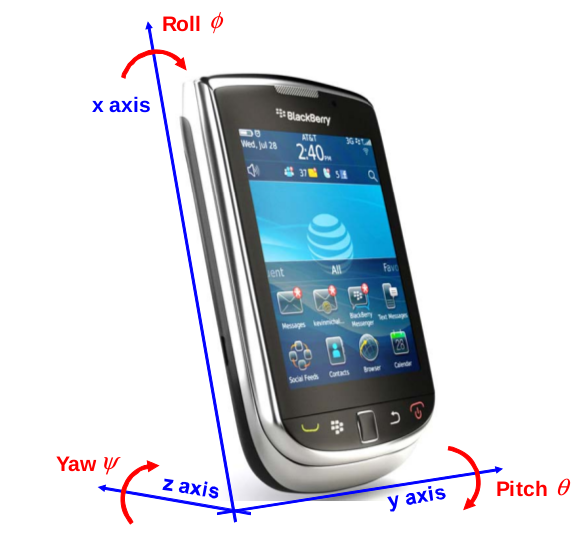
\includegraphics[width=8cm]{phone.png}
\caption{Axis Definitions for Accelerometer Measurement}
\label{f:phone}
\end{figure}
\begin{equation}
\mathbf{R}_{x}(\phi) = \begin{bmatrix}
1 & 0 & 0\\
0 & cos(\phi) & sin(\phi)\\
0 & -sin(\phi) & cos(\phi)
\end{bmatrix}
\label{e:rx}
\end{equation}
\begin{equation}
\mathbf{R}_{y}(\theta) = \begin{bmatrix}
cos(\theta) & 0 & -sin(\theta)\\
0 & 1 & 0\\
sin(\theta) & 0 & cos(\theta)
\end{bmatrix}
\label{e:ry}
\end{equation}
\begin{equation}
\mathbf{R}_{z} = \begin{bmatrix}
cos(\psi) & sin(\psi) & 0\\
-sin(\psi) & cos(\psi) & 0\\
0 & 0 & 1
\end{bmatrix}
\label{e:rz}
\end{equation}
\begin{equation}
\textbf{R}_{xyz}\begin{bmatrix}
0\\
0\\
1
\end{bmatrix} = \textbf{R}_{x}(\phi)\textbf{R}_{y}(\theta)\textbf{R}_{z}(\psi)\begin{bmatrix}
0\\
0\\
1
\end{bmatrix}
\end{equation}
For a 3-2-1 rotation sequence, $\mathbf{R}_{xyz}$, which represents the resulting rotation matrix, is obtained in Eq.(\ref{e:big}).
\begin{equation}
= \begin{bmatrix}
cos(\theta)cos(\psi) & cos(\theta)sin(\psi) & -sin(\theta)\\
cos(\psi)sin(\theta)sin(\psi) - cos(\phi)sin(\psi) & cos(\theta)cos(\psi) + sin(\theta)sin(\phi)sin(\psi) & cos(\theta)cos(\psi)\\
cos(\phi)cos(\psi)sin(\theta) + sin(\theta)sin(\psi) & cos(\phi)sin(\theta)sin(\psi) - cos(\psi)sin(\phi) & cos(\theta)cos(\phi)
\end{bmatrix}\begin{bmatrix}
0\\
0\\
1
\end{bmatrix}
\label{e:big}
\end{equation}
\begin{equation}
\textbf{R}_{xyz}\begin{bmatrix}
0\\
0\\
1\end{bmatrix} = \begin{bmatrix}
-sin(\theta)\\
cos(\theta)sin(\phi)\\
cos(\theta)cos(\phi)
\end{bmatrix} 
\end{equation}
Given a normalized accelerometer reading $\textbf{G}_{p}$:
\begin{equation}
\frac{\textbf{G}_{p}}{\| \mathbf{G}_{p} \|} = 
\frac{1}{\sqrt{G^{2}_{px} + G^{2}_{py} + G^{2}_{pz}}}\begin{bmatrix}
G_{px}\\
G_{py}\\
G_{pz}
\end{bmatrix}
=\begin{bmatrix}
-sin(\theta)\\
cos(\theta)sin(\phi)\\
cos(\theta)cos(\phi)
\end{bmatrix}=\Gamma_{phone}
\end{equation} 

Then, solving for the roll and pitch angles, $\phi$ and $\theta$ respectively yields the following solution:
\begin{equation}
tan(\phi_{xyz}) = \frac{G_{py}}{G_{pz}}
\end{equation}
\begin{equation}
tan(\theta_{xyz}) = \frac{-G_{px}}{G_{py}sin(\phi)+G_{pz}cos(\phi)}=\frac{-G_{px}}{\sqrt{G_{py}^{2} + G_{pz}^{2}}}
\end{equation}
\subsection{Attitude Matrix Method $\Gamma$}
The attitude matrix formulated method also looked at the misalignment matrix and worried about non-orthogonal rotations.  The tilt measured from the accelerometer cannot be related by a straightforward Euler angle rotation.  The Attitude Matrix Method instead looked at the tilt from the accelerometer as a roll ($\xi$), and pitch ($\psi$).  Note that in the previous derivation, these quantities were equal to $\phi$ and $\theta$ respectively.

\begin{figure}[h!]
\centering
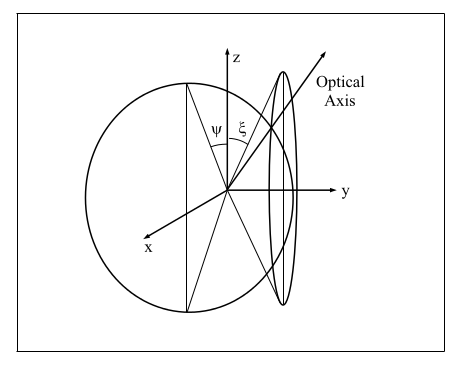
\includegraphics[scale=0.4]{cones.png}
\caption{Geometric Solution for off axis alignment}
\label{f:cones}
\end{figure}

Using geometry, this method models the difference between the rover zenith andj the new accelerometer reading as the intersection between two cones.  Looking at the equation of a sphere in $\mathbb{R}^{3}$.  
\begin{equation}
x^{2} + y^{2} + z^{2} = r^{2}
\end{equation}
If the roll angle is known, and the pitch angle is varied from 0 to $2\pi$, then the radius of the circle end of the cone is given by 

\begin{equation}
r = cos(\psi)
\end{equation}

Thus, the circle lies on the plane of $x = sin(\psi)$.  Substitution yields

\begin{equation}
y^{2} + z^{2} = r^{2} = 1 - sin^{2}(\psi)
\end{equation}

The same line of reasoning could be applied to the case where the pitch angle is known and the roll angle is varied to yield

\begin{equation}
x^{2} + z^{2} = r^{2} = 1 - sin^{2}(\xi)
\end{equation}

Since both of the points where the cones intersect will satisfy $x = sin(\psi)$ and $y = sin(\xi)$, z can be solved for.  Substitution yields
\begin{equation}
z = \pm \sqrt{1 - sin^{2}(\psi) - sin^{2}(\xi)}
\end{equation}

This means that the optical axis vector can be defined as follows

\begin{equation}
\vec{oa} = \begin{bmatrix} sin(\psi) & sin(\xi) & \sqrt{1 - sin^{2}(\psi) - sin^{2}(\xi)}  \end{bmatrix}
\label{e:oavector}
\end{equation}

From here, the derivation used the properties of orthogonal vectors to determine the other two orthogonal optical axes.  The equations are shown below

\begin{equation}
y \cdot z = 0
\end{equation}

\begin{equation}
x \cdot z = 0
\end{equation}

\begin{equation}
y \cdot x = 0
\end{equation}

\begin{equation}
y \times z = x
\end{equation}

\begin{equation}
x \cdot x = 1
\end{equation}

\begin{equation}
y \cdot y = 1
\end{equation}

Then, the generated vector components are normalized and put into final matrix form

\begin{equation}
\Gamma = \begin{bmatrix}
x\\
y\\
z
\end{bmatrix} = \begin{bmatrix}
y\times z \\
y\\
z
\end{bmatrix}
\end{equation}
\subsection{Failure Conditions for Zenith Requirement Solution}
Eq.~(\ref{e:oavector}) has a failure condition.  As $sin^{2}(\psi)+sin^{2}(\xi)$ approaches $1$, the third term of the vector enters the complex domain.  That is, wherever $sin^{2}(\psi)+sin^{2}(\xi)>1$, the function defining the optical axis z-component no longer has a real value, despite that z may be greater than zero for a given pitch and roll. This suggests that the solution does not produce valid results for useful angles of pitch and roll. Combinations of pitch and roll angles that follow this condition can be seen in Fig.~\ref{f:failure}.
\begin{figure}[!ht]
\centering
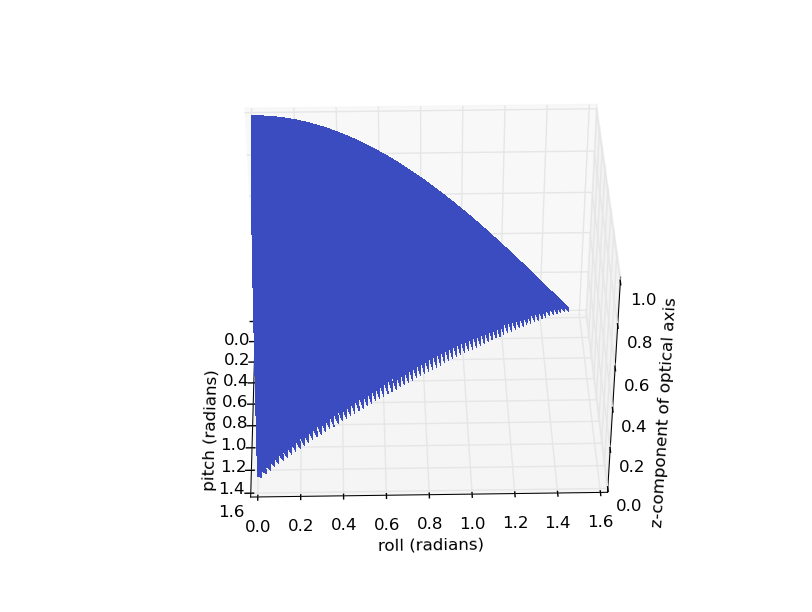
\includegraphics[height=8cm]{zenithFail.png}
\caption{Real components of $\sqrt{1-sin^{2}(\psi)-sin^{2}(\xi)}$.  The area of the roll-pitch plane where no z axis value is present is an area in which the optical axis z component does not take on a real value.}
\label{f:failure}
\end{figure}
It can be seen from the experimental verification of the CST that the orientation angle of the the CST from the vertical never varied by more than approximately 2 degrees. This shows that although CST was not pointed at full zenith, it did not appear to examine a wide range of angles to prove that the zenith requirement could be eliminated.  A table depicting the pointing angles of CST is shown in Fig~\ref{f:alt}.
\begin{figure}[!ht]
\centering
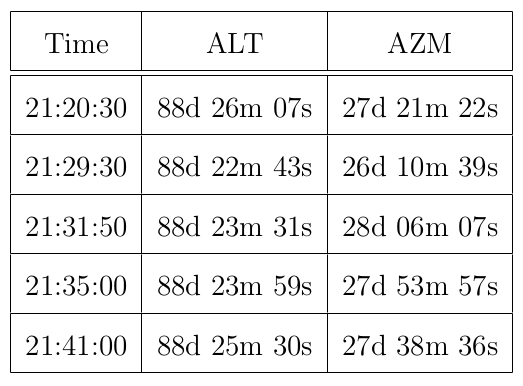
\includegraphics[height=4cm]{altitude.png}
\caption{Altitude (Zenith) Angle Orientation of CST}
\label{f:alt}
\end{figure}
The inflexibility of the zenith requirement, along with the apparent failure condition of the equation that removes the zenith requirement from CST led to the development of a new algorithm, based on maritime techniques.  \\
\FloatBarrier
\subsection{Miscellaneous Corrections to Attitude Matrix Method}
For improved accuracy of the algorithm, and since, for proof of concept, the algorithm will be tested on the Earth, further corrections must be made.  One way to model the refraction that the Earth's atmosphere applies to the incoming starlight is by using Snell's Law \cite{b:knight}.  Even though the Earth's atmosphere is a continuum that dissipates as altitude is increased, we model it the atmosphere as a continuous boundary, like when a cup refracts the light of a straw. Snell's Law is depicted in Fig.~\ref{f:snells} and given as:

\begin{equation}
n_{1}\sin(\theta_{1}) = n_{2}\sin(\theta_{2})
\end{equation}
where $n_{1}$, and $n_{2}$ are the indices of refraction for the two mediums, $theta_{1}$ and $theta_{2}$ are the angle of incidence, and the angle of refraction, respectively. 

For optical axis angels that are less than $45^{\circ}$ from zenith, the angle of refraction $\theta = \theta_{1} - \theta_{2}$ can be approximated as

\begin{equation}
\theta = (n_{2} - 1)\tan(\theta_{2})
\end{equation}
\begin{figure}[h!]
\centering
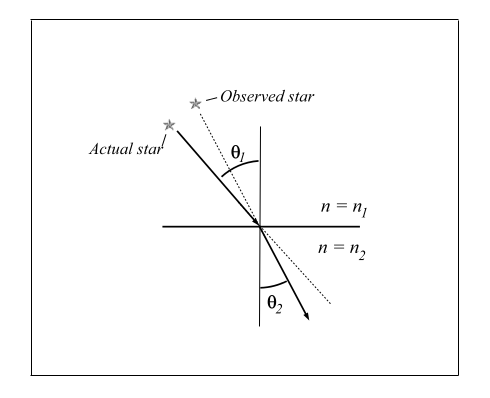
\includegraphics[scale=0.4]{snells.png}
\caption{Snell's Law and Atmospheric Aberration Effect}
\label{f:snells}
\end{figure}
The angular correction for angles from aligned with zenith (0 rads) to $45^{\circ}$ is shown in Fig.~\ref{f:snellgraph}.
\begin{figure}[h!]
\centering
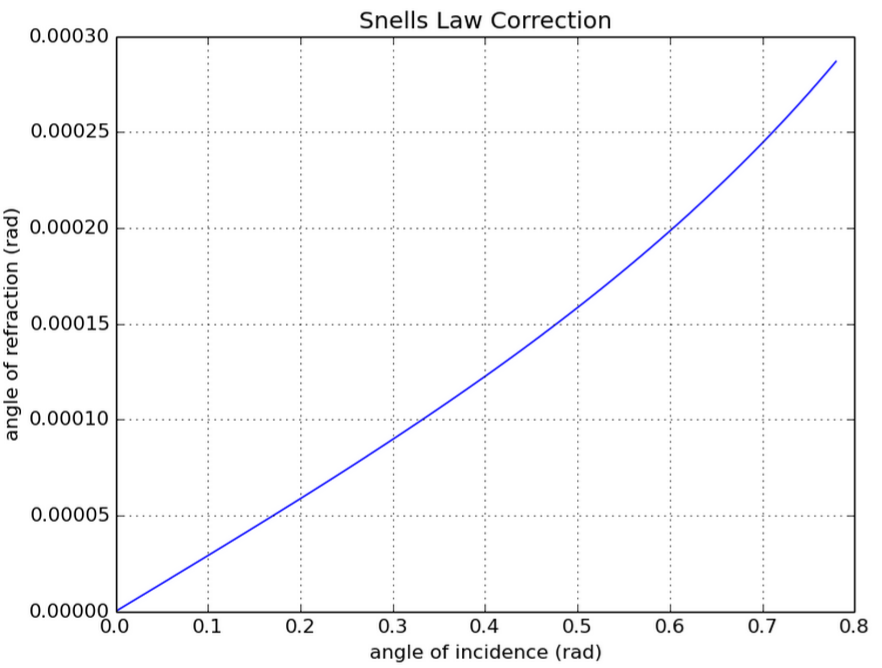
\includegraphics[width=8cm]{snellGraph.png}
\caption{Plot of Angle of Incidence vs. Angle of Refraction for Snell's Law}
\label{f:snellgraph}
\end{figure}
The other major matrix that is constructed as part of the Attitude Matrix Method is the $A^{G/I}$ matrix.  These corrections are important because it is possible to model the irregular swaying of the Earth's rotational axis. Fabricating this matrix is challenging because the translation between Greenwich to Inertial coordinate frames depends on many physical factors that are not easy to predict.  The main components for this matrix are the nutation and precession.  The other secondary components are the Greenwich angle $\psi$ and the Earth orientation parameters, which are also referred to as the polar motion. Fig.~\ref{f:nutpress} shows what nutation and precession look like with respect to a planetary body's rotational axis.

\begin{figure}[h!]
\centering
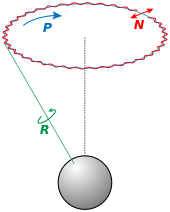
\includegraphics[scale=0.5]{NP.png}
\caption{Nutation and Precession}
\label{f:nutpress} %LMAO
\end{figure}

Here, P shows the precession, or the minute circular motion the Earth tends to take over a long period of time, and N shows the nutation, or the oscillations within that circular path.  Vallado created a curve fitting method that allows the nutation and precession of the Earth to be modeled as follows \cite{b:vallado}.

\begin{equation}
NP = R_{1}(-\alpha)R_{3}(-\beta)R_{1}(\gamma)R_{3}(\delta)
\end{equation}

$\gamma$ and $\delta$ are define the location of the ecliptic pole in the inertial frame, $\beta$ is the ecliptic angle of precession, and $\alpha$ is the obliquity of the ecliptic.  These angles are all functions of time and are defined as follows.

\begin{equation}
\alpha = (84381.4428 - 46.8388t - 0.0002t^{2} + 0.002t^{3})/3600
\end{equation}

\begin{equation}
\beta = (-0.0431 + 5038.4739t + 1.5584t^{2} - 0.0002t^{3})/3600
\end{equation}

\begin{equation}
\gamma = (84381.4479 - 46.814t + 0.0511t^{2} + 0.0005t^{3})/3600
\end{equation}

\begin{equation}
\delta = (10.5525t + 0.4932t^{2} - 0.0003t^{3})/3600
\end{equation}

In these equations, time is calculated as a function of the Julian Date, as given in the following equation
\begin{equation}
t = \frac{JD-T_{0}}{T_{century}}
\end{equation}

here, JD is the Julian Date, $T_{0}$ is the Julian Date at J2000 $(T_{0} = 2451545)$, at $T_{century}$ is equal to 36525, or the number of days in one century.

\section{Proposed Algorithm}
\subsection{Blind Astrometric Nautical Sight Reduction}
The proposed method is a computer vision based method that combines the Blind Astrometric Calibration Method, the Center Pixel Method, and the Direct Computation Method for Nautical Sight Reduction \cite{b:naut}.  This method measures the angle between the horizon and star.  This angle is known as the altitude.  The algorithm requires an optical light image of the stars. The raw image from Fig.~\ref{f:im60} is processed by the astrometry software.  An example result of ``image 60", used for actual position determination, is shown in Fig.~\ref{f:im60a}. The astrometry package is a complicated piece of software, which uses image processing, geometric methods, and access to the USNO-B star catalog for determination of the celestial bodies in the image \cite{b:astro}.  A high level overview of the Blind Astrometric Nautical Sight Reduction Algorithm is shown below in Fig.~\ref{f:diagram}.
\begin{figure}[!ht]
\centering
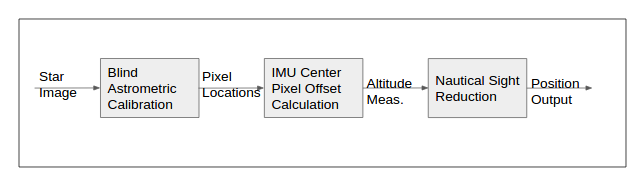
\includegraphics[width=12cm]{diagram.png}
\caption{Top Level Block Diagram of New Algorithm}
\label{f:diagram}
\end{figure}

\begin{figure}[!ht]
\centering
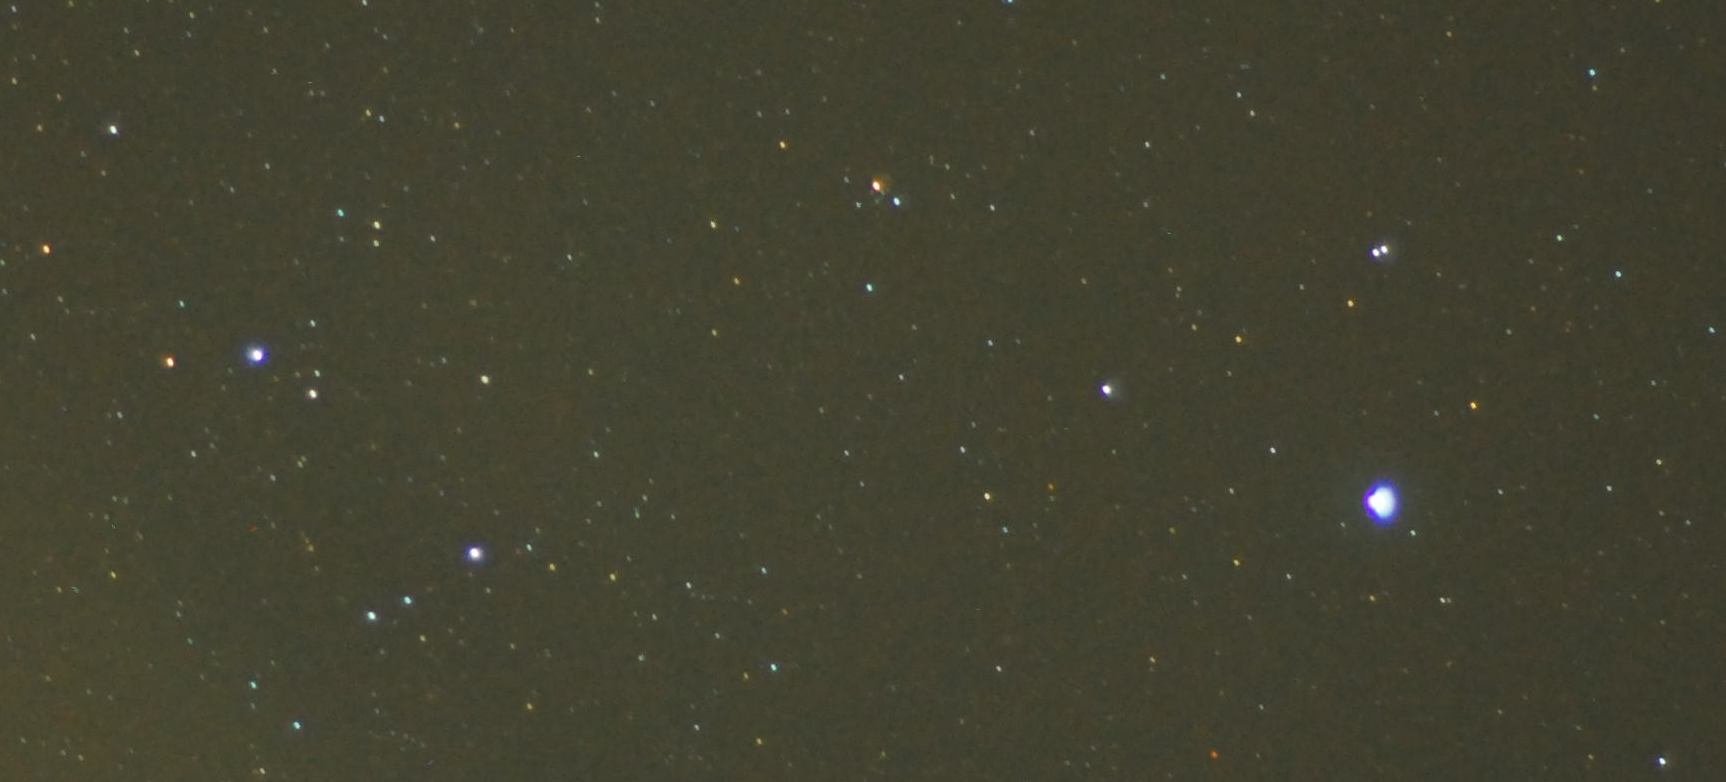
\includegraphics[width=12cm]{im60.png}
\caption{Example image taken by star tracker.}
\label{f:im60}
\end{figure}
\begin{figure}[!ht]
\centering
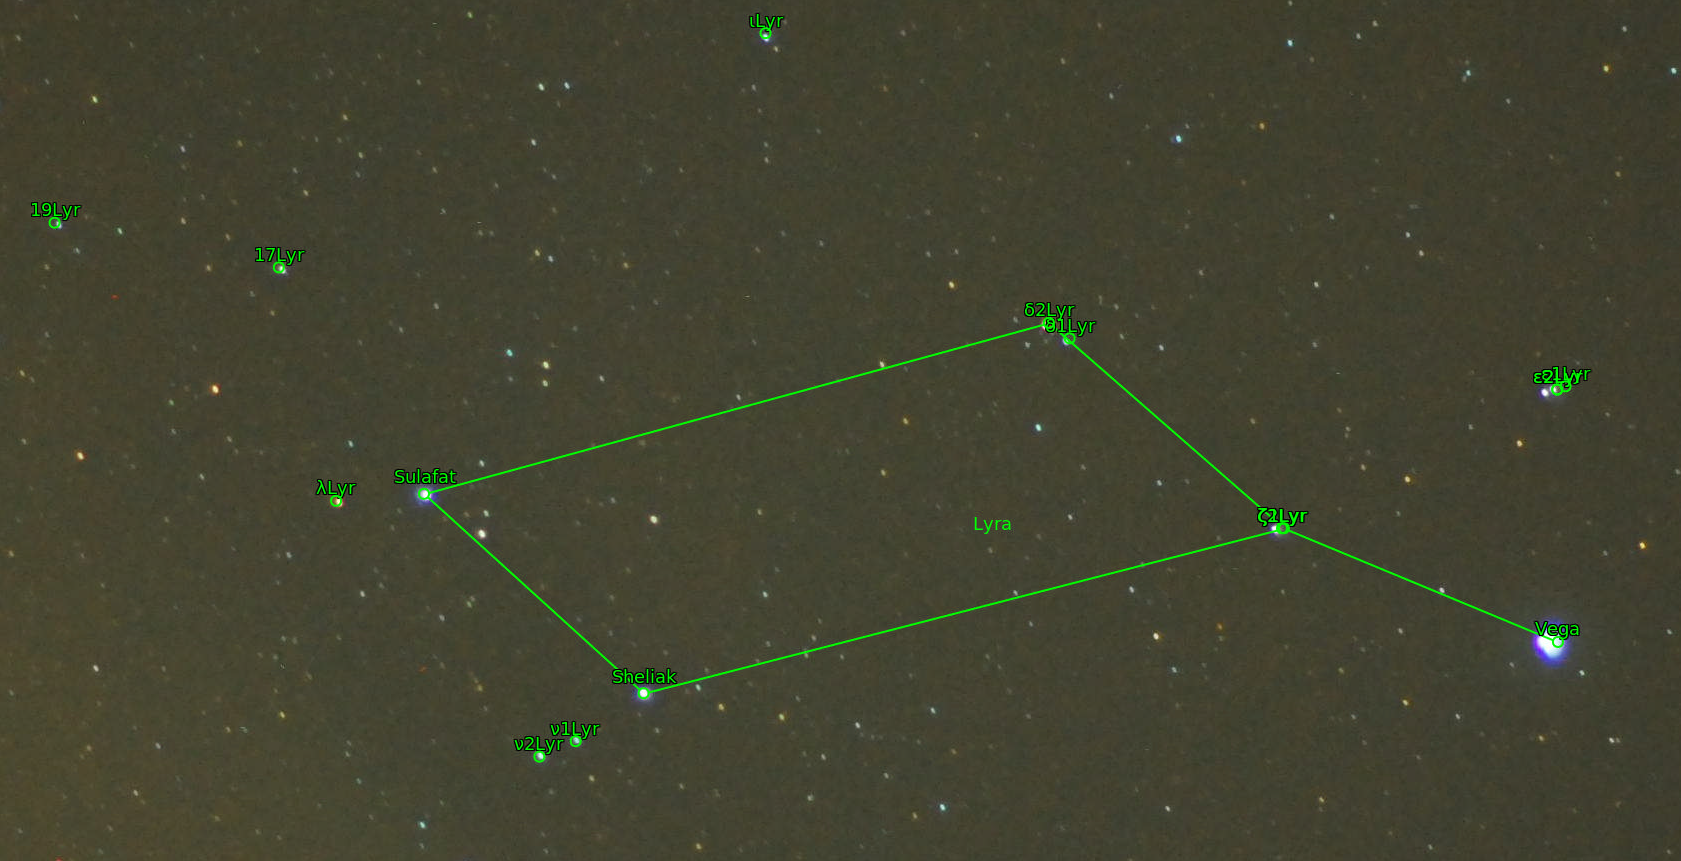
\includegraphics[width=12cm]{im60a.png}
\caption{Example image after processing by Astrometry software package.}
\label{f:im60a}
\end{figure}
\FloatBarrier
The algorithm begins with an estimation of the initial position of the mobility solution. The local hour angle is computed as the addition of Greenwich hour angle (GHA), and the current longitude, \textit{Long}.  
\begin{equation}
 \label{e:LHA}
    LHA = GHA + Long
\end{equation}
$H_{c}$ is the altitude of the observed star if the estimated position was the true location.  $H_{c}$ can be calculated as follows.

\begin{equation}
 \label{e:Hc}
    H_{c} = \sin^{-1}(S\sin(Lat) - C\cos(Lat))
\end{equation}
In equation~(\ref{e:Hc}), S is defined as $S = \sin(Dec)$ and C is defined as $C = \cos(Dec)\cos(LHA)$.
X, and A are parameters which are used to determine the azimuth direction, and are calculated as follows.
\begin{equation}
 \label{e:X}
    X = \frac{S\cos(Lat) - C\sin(Lat)}{\cos(H_{c})}
\end{equation}

\begin{equation}
 \label{e:A}
    A = \cos^{-1}(X)
\end{equation}
In Eq.~(\ref{e:A}), if $LHA > 180^{\circ}$, then set Z = A.  Otherwise, $Z = 360^{\circ} -A$.  The next portion of the sight reduction method is an iterative method which calculates ground distance between the estimated point from $H_c$ and the observed point found with $H_{o}$, known as $p$.  $H_{o}$ is the measured altitude of the star.  The quantity $p$ is also referred to as the intercept Eq.~(\ref{e:p}).  In this research, the quantity is also referred to interchangeably as $\Delta H$. 

\begin{equation}
 \label{e:p}
    p = H_{o} - H_{c}
\end{equation}

Fig.~\ref{f:pdeltah} depicts the Nautical Sight Reduction method, and in particular Eq.(~\ref{e:p}).  

\begin{figure}[!ht]
\centering
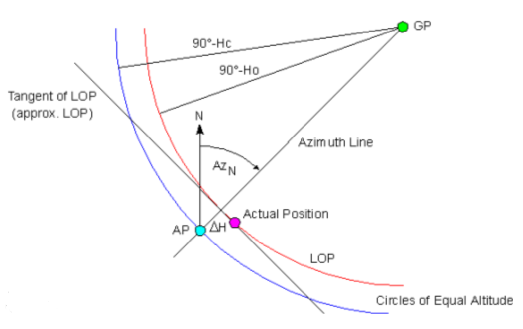
\includegraphics[width=12cm]{pdeltah.png}
\caption{Diagram of Sight Reduction.  Note $\Delta H$ on this figure is defined as $p$ in this research \cite{b:celnavde}}
\label{f:pdeltah}
\end{figure} 
\FloatBarrier
\subsection{Center Pixel Method}
Calculation of $H_{o}$ is performed by assigning IMU pitch and roll values to the image center pixel.  This is shown in Eq.~(\ref{e:cpm1}) where the variables are in units of pixels.
\begin{equation}
    \label{e:cpm1}
       \begin{pmatrix} 
  x_{T}     \\ 
  y_{T} 
\end{pmatrix}=\begin{pmatrix} 
  \cos(\theta)     & -\sin(\theta)\\ 
  \sin(\theta) & \cos(\theta) 
\end{pmatrix}\begin{pmatrix} 
  x\\ 
  y_{c} + y_{off} 
\end{pmatrix}
\end{equation}
Now that $Z$ and $p$ for each observation are calculated, the terms from the iterative method can be calculated. The terms, A,B,C,D,E and G of each summation are used to calculate the center of the error polygon used for navigation.  Note that $n$ represents the number of observations.  The terms are defined in as follows:

\begin{equation}
A = \sum \limits_{i=1}^n \cos^{2}Z_{i}
\end{equation}
\begin{equation}
B = \sum \limits_{i=1}^n \cos Z_{i} \sin Z_{i}
\end{equation}
\begin{equation}
C = \sum \limits_{i=1}^n \sin^{2}Z_{i}
\end{equation}
\begin{equation}
D = \sum \limits_{i=1}^n p_{i}cosZ_{i}
\end{equation}
\begin{equation}
E = \sum \limits_{i=1}^n p_{i}sinZ_{i}
\end{equation}
These terms can then be combined as follows. Note $B_{I}$ and $B_{F}$ are the improved and estimated latitude respectively.  $L_{I}$ and $L_{F}$ are the improved and estimated longitude respectively.  $d$ is the distance in nautical miles between $(L_{F}, B_{F})$ and $(L_{I}, B_{I})$.  This value is expected to converge as the number of iterations increase, indicating that a final position estimate is obtained.
\begin{equation}
 \label{e:G}
    G = AC-B^{2}
\end{equation}

\begin{equation}
 \label{e:Bi}
    B_{i} = B_{F} + \frac{CD-BE}{G}
\end{equation}

\begin{equation}
 \label{e:Li}
    L_{i} = L_{f} + \frac{AE - BD}{Gcos(B_{F})}
\end{equation}

\begin{equation}
 \label{e:d}
    d = 60\sqrt{(L_{I} - L_{F})^{2}cos^{2}(B_{F}) + (B_{I} - B_{F})^{2}}
\end{equation}
%In Eq. In Eq.~(\ref{e:Bi}), and Eq.~(\ref{e:Li}), the subscript ``I" refers to an ``improved" guess, and the subscript ``F" refers to a an initial guess.  
The algorithm is repeated until the value of Eq.~(\ref{e:d}) is sufficiently small.  The process is depicted in the convenient diagram form of Fig.~\ref{f:nsrBlocks}.  It is expected that the zenith requirement and backtracker method will be eliminated by the correct implementation of this algorithm.
\begin{figure}[h!]
\centering
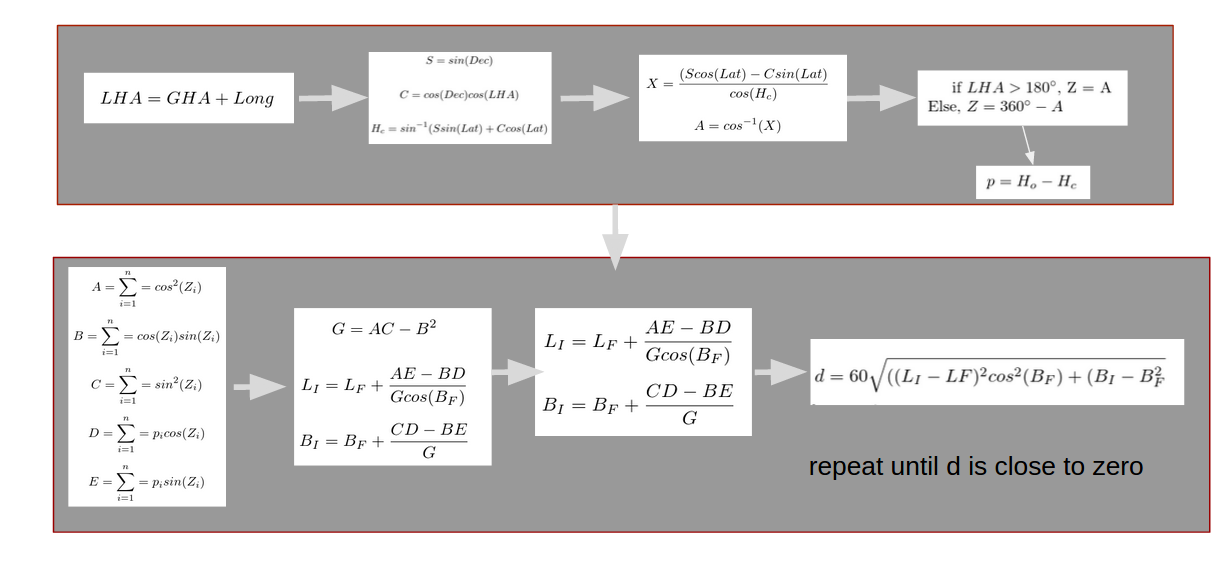
\includegraphics[scale=0.35]{nsrBlocks.png}
\caption{Diagram Form of Nautical Sight Reduction Algorithm}
\label{f:nsrBlocks} 
\end{figure}

\chapter{Simulations of Nautical Sight Reduction Algorithm}
Simulations were performed to demonstrate the use of the nautical sight reduction method.  These simulations also show convergence and accuracy of three different observation formats.  \textbf{Case 1} sights three stars sighted at three different times.  \textbf{Case 2} sights three stars from the same image. \textbf{Case 3} sights a single star from three different images, taken at three different times.  Tables ~\ref{t:case1} and ~\ref{t:case2} depict the right ascension and declination of Case 1 and Case 2, repsectively.  Table ~\ref{t:summerTri} shows the right ascension and declination of the summer triangle.  This includes the data on the star Altair, which comprises Case 3.  The values of right ascension and declination were obtained from the Hipparcos star catalog ~\cite{b:hipp}.  
\begin{table}[ht!]
\centering
\begin{tabular}{ |c|c|c|c| } 
 \hline
 . & Regulus & Antares & Kochab \\ 
 \hline
 Right Ascension & 10h08m22s & 16h29m25s & 14h50m25s \\ 
 \hline
 Declination & $11^{\circ}58^{'}$ & $-26^{\circ}25^{'}$ & $74^{\circ}09^{'}$ \\ 
 \hline
\end{tabular}
\caption{Right Ascension and Declination of Stars Observed in Case 1}
\label{t:case1}
\end{table}

\begin{table}[ht!]
\centering
\begin{tabular}{ |c|c|c|c| } 
 \hline
 . & Sulafat & Sheliak & Vega\\ 
 \hline
 Right Ascension & 18h58m56s & 18h50m04s & 18h36m56s \\ 
 \hline
 Declination & $32^{\circ}41^{'}$ & $33^{\circ}21^{'}$ & $38^{\circ}47^{'}$ \\ 
 \hline
\end{tabular}
\caption{Right Ascension and Declination of Stars Observed in Case 2}
\label{t:case2}
\end{table}

\begin{table}[ht!]
\centering
\begin{tabular}{ |c|c|c|c| } 
 \hline
 . & Altair & Deneb & Vega\\ 
 \hline
 Right Ascension & 19h50m46s & 20h41m26s & 18h36m56s \\ 
 \hline
 Declination & $08^{\circ}52^{'}$ & $45^{\circ}16^{'}$ & $38^{\circ}47^{'}$ \\ 
 \hline
\end{tabular}
\caption{Right Ascension and Declination of Stars Observed in Case 3 and Summer Triangle}
\label{t:summerTri}
\end{table}
\FloatBarrier
The stars of the summer triangle were sighted concurrently from Durham, NH, ($70.9349^{\circ}W$, $43.1338^{\circ}N$). This test was used in a simulation of algorithm convergence only. In Case 1, the stars were sighted from $15^{\circ} E$, $32^{\circ} N$.  For this format, the time intervals between sightings are 6 and 25 minutes. Simulations of Case 2 and Case 3 are sighted from Durham, NH ($70.9349^{\circ}W$, $43.1338^{\circ}N$).  In Case 3, each image of Altair was simulated to be approximately 8 minutes apart.

\section{Convergence}
The first test of each observation format is to determine whether or not Eq.~(\ref{e:d}) converges to a single value.  The algorithm was tested over ten iterations with no additional noise or bias. In Figure~\ref{f:converge} it can be seen that in general each observational format converges by the second iteration. 
\begin{figure}[!ht]%2
\centering
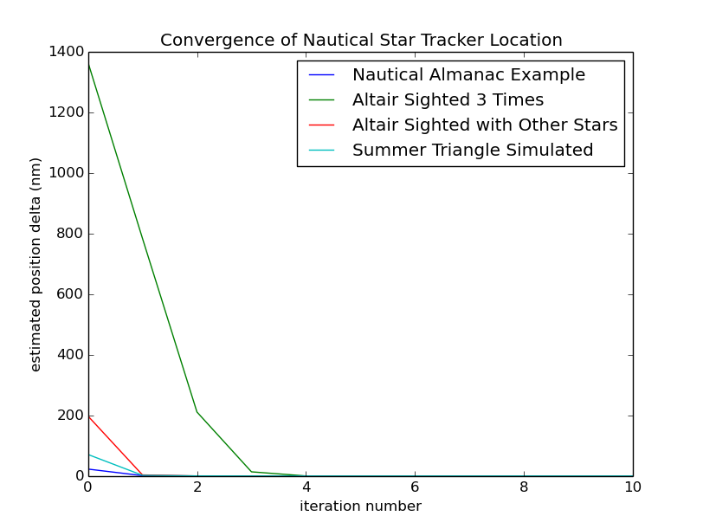
\includegraphics[height=8cm]{convergence.png}
\caption{Convergence of the different observational schemes.}
\label{f:converge}
\end{figure}
Case 3 takes four iterations to converge.  This suggests that method may be suboptimal for navigation.
\section{Position Estimation}
Each of the formats was examined for accuracy of position estimation.  The simulation was run 1000 times, and iterated over Eq.(\ref{e:d}) 10 times.  The desired result is to determine the correct altitude measurements for each of the three cases, from which correct position can be obtained. No noise or bias is added to the altitudes in the position estimation simulations. The results and corresponding histograms are presented. Each histogram has a total of 1000 observations, each having the same value. Table ~\ref{t:colorz} depicts the legend information for plots of this section.  
\begin{table}[ht!]
\centering
\begin{tabular}{ |c|c|c|c| } 
 \hline
 Blue & Red & Green & Teal\\ 
 \hline
 Position Est. & N/A & N/A & True Value \\ 
 \hline
\end{tabular}
\caption{Legend Format for Position Estimate Plots}
\label{t:colorz}
\end{table}
\subsection*{Case 1:  Three Stars, Three Times}
The histogram of position estimates corresponding to the stars Kochab, Regulus and Antares observed from $15^{\circ} E$, $32^{\circ} N$ at different times from  are shown in Fig.~\ref{f:3s3t_z_z}.  The map of these estimates is shown in Fig.~\ref{f:3s3t_z_z_map}.  These results suggest that observing three stars a single time is a potentially viable method for position determination.
\begin{figure}[!h]%2
\centering
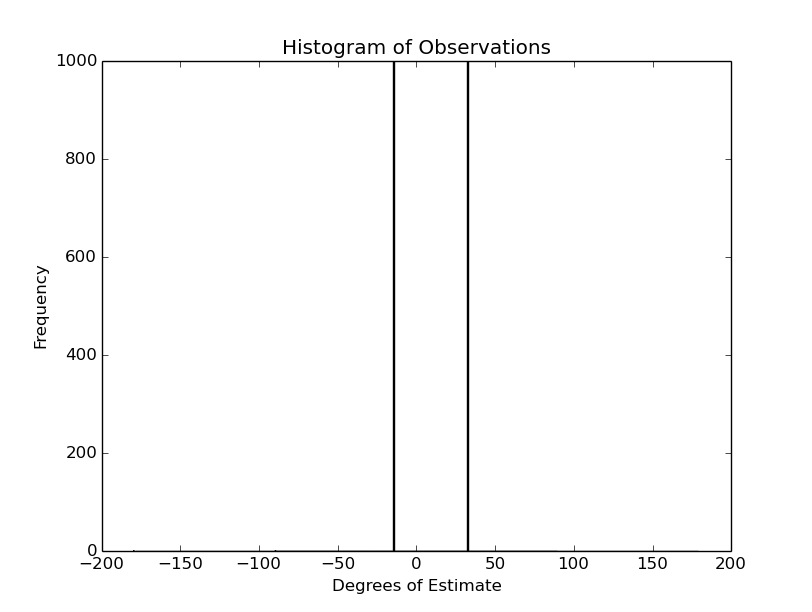
\includegraphics[height=8cm]{3s3t_z_z.png}
\caption{Case 1 Histogram of Position Estimates}
\label{f:3s3t_z_z}
\end{figure}
\begin{figure}[!h]%2
\centering
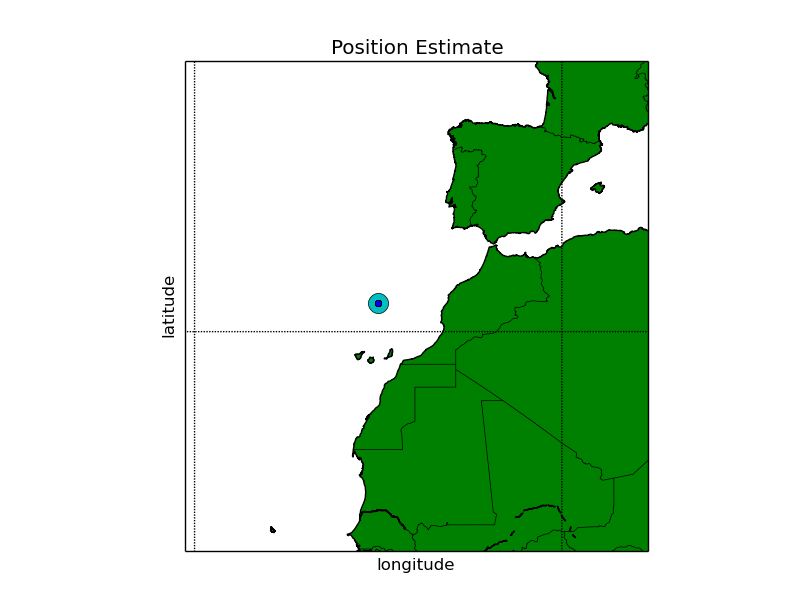
\includegraphics[height=8cm]{3s3t_z_z_map.png}
\caption{Case 1 Map of Position Estimates}
\label{f:3s3t_z_z_map}
\end{figure}
\FloatBarrier

\subsection*{Case 2: Three Stars, One Time}
The histogram of position estimates corresponding to the stars Sheliak, Sulafat, and Vega observed at the same time, (UTC-01:09:00) is shown in Fig.~\ref{f:3s1t_z_z}.  The map of these estimates is shown in Fig.~\ref{f:3s1t_z_z_map}. These results suggest that observing three stars a single time is a potentially viable method for position determination. 
\begin{figure}[!h]%2
\centering
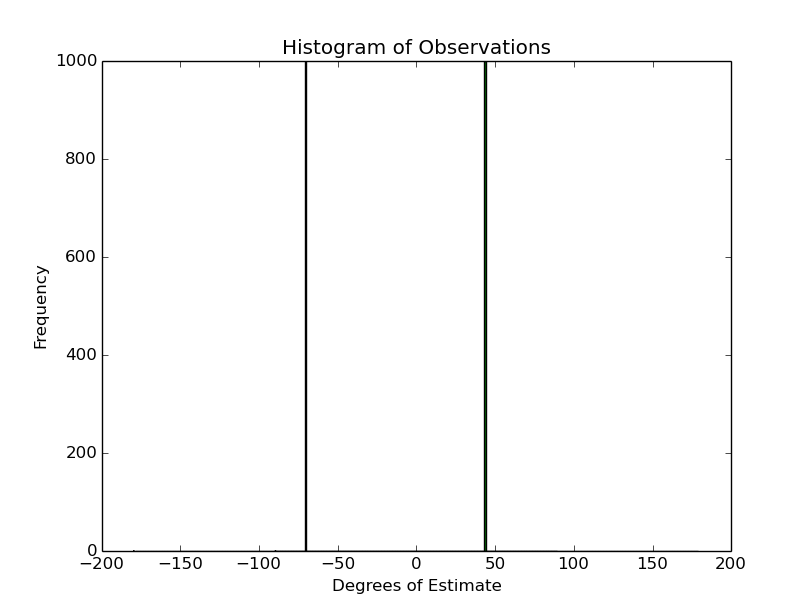
\includegraphics[height=8cm]{3s1t_z_z.png}
\caption{Case 2 Histogram of position estimates.}
\label{f:3s1t_z_z}
\end{figure}
\begin{figure}[!h]%2
\centering
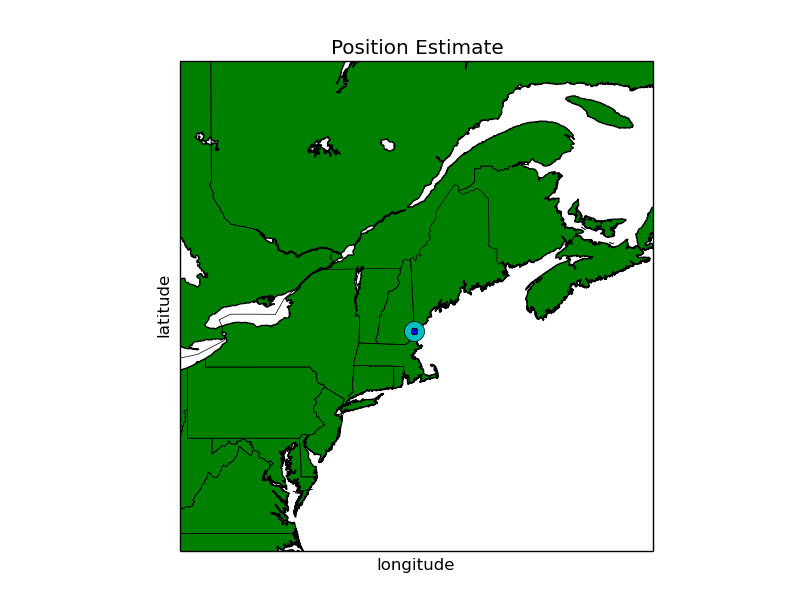
\includegraphics[height=8cm]{3s1t_z_z_map.png}
\caption{Case 2 Map of Position Estimates.}
\label{f:3s1t_z_z_map}
\end{figure}
\FloatBarrier


\FloatBarrier
\subsection*{Case 3: One Star, Three Times} 
The histogram of position estimates corresponding to the star Altair observed three different times is shown in Fig.~\ref{f:1s3t_z_z}.  The corresponding map is shown in Fig.~\ref{f:1s3t_z_z_map}.  These results suggest that observing a single star one time is a potentially viable method for position determination.
\begin{figure}[!h]%2
\centering
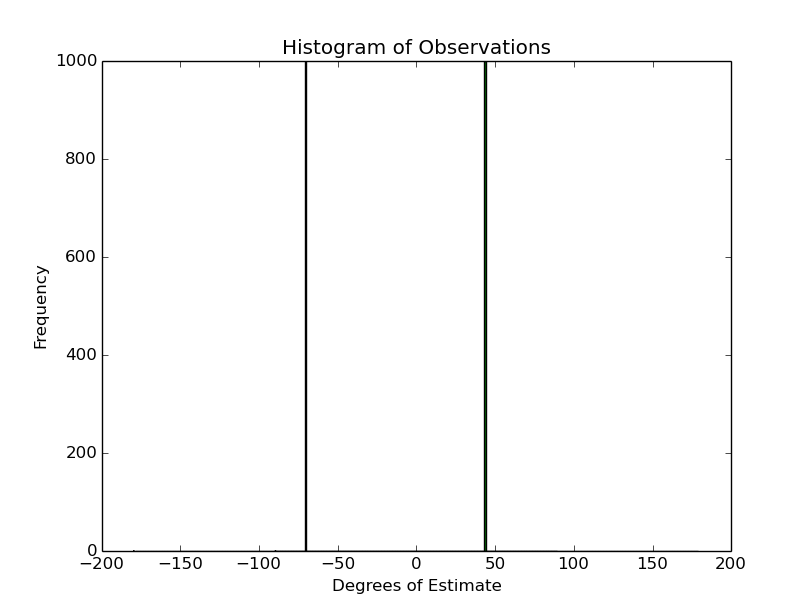
\includegraphics[height=8cm]{1s3t_z_z.png}
\caption{Case 3 Histogram of Position Estimates}
\label{f:1s3t_z_z}
\end{figure}
\begin{figure}[!h]%2
\centering
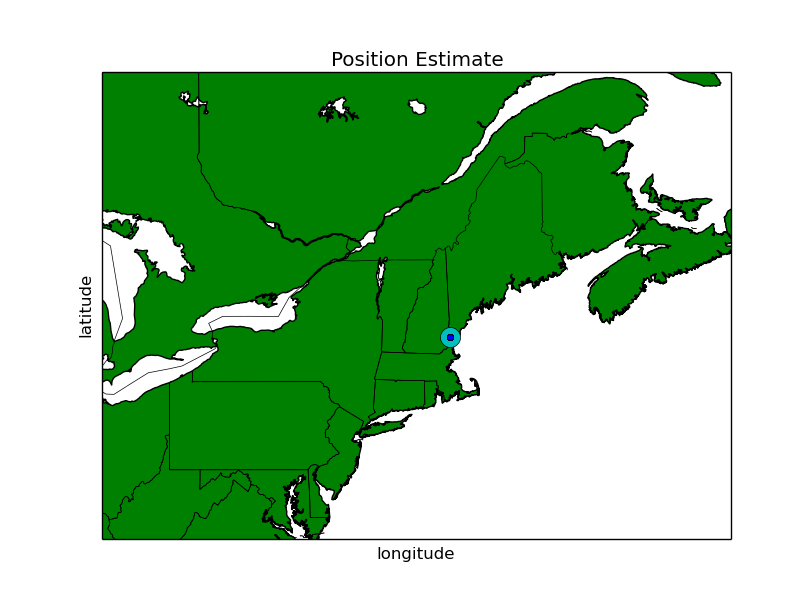
\includegraphics[height=8cm]{1s3t_z_z_map.png}
\caption{Case 3 Map of Position Estimates}
\label{f:1s3t_z_z_map}
\end{figure}

\FloatBarrier
\section{Noise in Observed Altitudes}
A uniform distribution of noise was added to each observation to determine the effect of random noise on position estimate.  The uniform distribution was chosen because it enabled easy to implement noise bounds while retaining the mean as an accurate measure of the distribution center.  Additionally, this distribution imposes a more strict requirement on the star camera noise bounds so that a greater accuracy may eventually be obtained.  The probability density function of this distribution is described in Eq.~(\ref{e:distribution}).  A plot of a histogram developed using this distribution is shown in Fig.~\ref{f:uniHist}.  
\begin{equation}
p(x) = \frac{1}{b-a}
\label{e:distribution}
\end{equation}

\begin{figure}[!h]%2
\centering
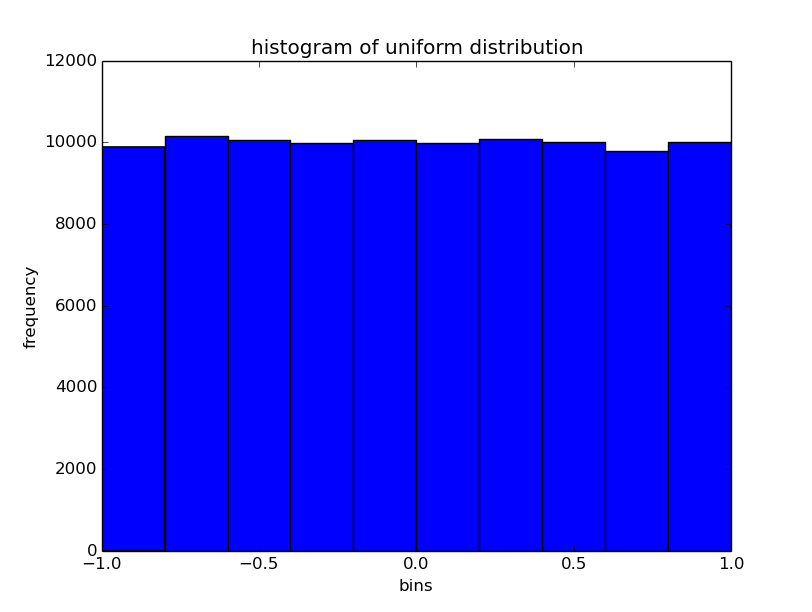
\includegraphics[height=8cm]{uniHist.png}
\caption{Uniform Probability Density Histogram}
\label{f:uniHist}
\end{figure}
\FloatBarrier
Table ~\ref{t:colorz2} depicts the legend of the plots for this section.

\begin{table}[ht!]
\centering
\begin{tabular}{ |c|c|c|c| } 
 \hline
 Blue & Red & Green & Teal\\ 
 \hline
 $\pm 1^{\circ}$ & $\pm 2^{\circ}$& $\pm 5^{\circ}$ & True Value \\ 
 \hline
\end{tabular}
\caption{Legend of Noisy Position Estimate Plots}
\label{t:colorz2}
\end{table}
Studies of the noise examine the geometric distribution of the estimated points and determine if the mean of the estimates yields the correct position.  For each data point generated in the study, a simulated array of three altitude measurements, $H_{o,1}$, $H_{o,2}$, and $H_{o,3}$ are generated.  
Two cases were studied.  The boundaries $(a,b)$ for the noise $\epsilon_{i}$ were chosen to be $\pm 1$,$\pm 2$, and $\pm5 $ degrees. In the uniform case, the same amount of noise is added to each star altitude measurement such that, for an additional noise value $\epsilon_{i}$, the altitudes are input to Nautical Sight Reduction as depicted in Eq.~(\ref{e:noise1}).
\begin{equation}
\begin{bmatrix}
H_{o,1,new} \\
H_{o,2,new}\\
H_{o,3,new}
\end{bmatrix} = 
\begin{bmatrix}
H_{o,1} + \epsilon_{1}\\
H_{o,2} + \epsilon_{1}\\
H_{o,3} + \epsilon_{1}
\end{bmatrix}
\label{e:noise1}
\end{equation}
The expected effect of the uniform simulation of uniform noise is that the values of noise will function similar to a value of bias.  If the same constant value $\epsilon_{1}$ is added to each $H_{o,i}$ of an observation, the circles of equal altitude will increase for $-\epsilon_{1}$ and decrease for $+\epsilon_{1}$.
In the non-uniform case, a different amount of noise is added to each observation, described in Eq.~(\ref{e:noise2}).
\begin{equation}
\begin{bmatrix}
H_{o,1,new} \\
H_{o,2,new}\\
H_{o,3,new}
\end{bmatrix} = 
\begin{bmatrix}
H_{o,1} + \epsilon_{1}\\
H_{o,2} + \epsilon_{2}\\
H_{o,3} + \epsilon_{3}
\end{bmatrix}
\label{e:noise2}
\end{equation}
The expected effect of a non-uniform noise is that the distribution of points will take up more area.  This is because position estimate determined by Eq.~(\ref{e:Bi}), and Eq.~(\ref{e:Li}) is determined by taking the centroid of the spherical error polygon. As the radius one of the circles of position change due to the value of $\epsilon_{i}$, the estimated position will also change. 


%determine how this goes
\subsection*{Case 1: Three Stars, Three Times}
Fig.~\ref{f:3s3t_case1} and Fig.~\ref{f:3s3t_case2} depict the uniform and non-uniform noise on the observations of Kochab, Antares, and Regulus.  
\FloatBarrier
\begin{figure}[!h]%2
\centering
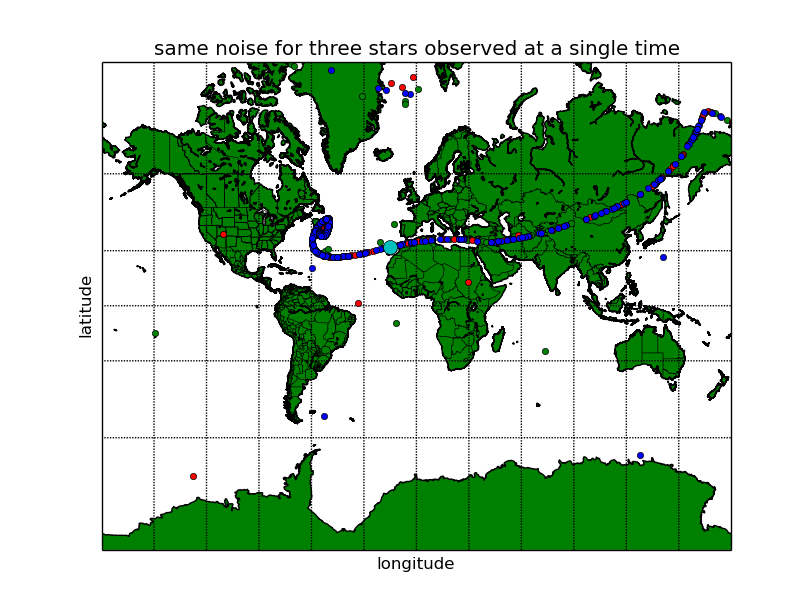
\includegraphics[height=8cm]{3s3t_case1.png}
\caption{Distribution of Estimates for Case 1 Observation Format: Uniform Noise Simulation}
\label{f:3s3t_case1}
\end{figure}
\begin{figure}[!h]%2
\centering
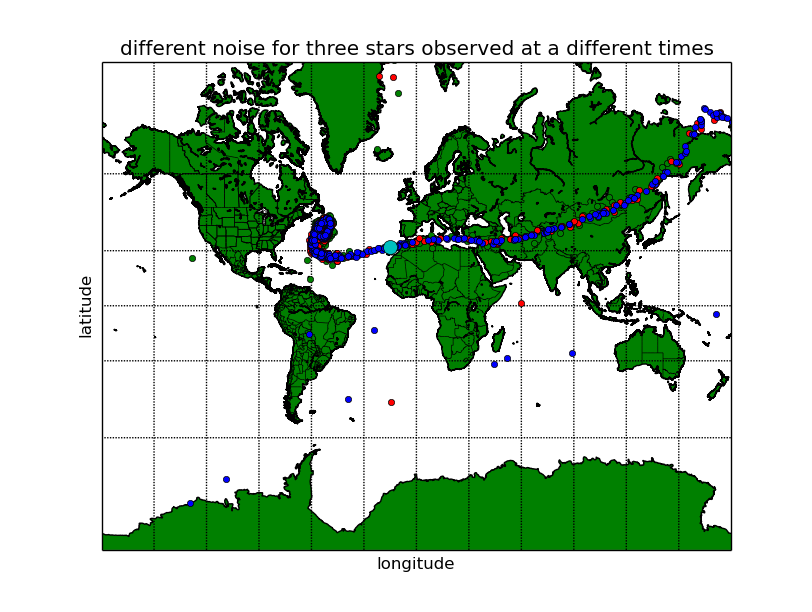
\includegraphics[height=8cm]{3s3t_case2.png}
\caption{Distribution of Estimates for Case 1 Observation Format: Non-Uniform Noise Simulation}
\label{f:3s3t_case2}
\end{figure}
\FloatBarrier
One of the most notable effects of this format, especially as compared to the other formats studied of this chapter are that the distribution of the estimates has the same shape for both the uniform and non-uniform noise simulations.  One reason for the interesting curvature may be that the stars are in different parts of the sky compared to the stars of the other two observational formats.  The right ascensions and declinations of Regulus, Antares, and Kochab are given in Table ~\ref{t:case1}.  This format was observed to have a large number of non-convergent values. If the lines of position, as calculated from Eq.~(\ref{e:p}) and Eq.~(\ref{e:A}) do not intersect, then a position estimate is not able to be obtained using this observational format.  The presence of such nonconvergent values infers that Case 1 is not appropriate for practical use until further study can be performed.

\FloatBarrier
\subsection*{Case 2: Three Stars, One Time}
\FloatBarrier
Fig.~\ref{f:3s1t_single_total_noise} depicts the estimated position given the same amount of uniform random noise added to each of the three stars observed.  Fig.~\ref{f:3s1t_case2_noise} depicts the estimated positions given different amounts of uniform random noise for each star.  It can be observed that a uniform noise offsets the position estimate in a linear fashion.  The centroid of the distribution of estimates represents the true point.

In Fig.~\ref{f:3s1t_case2_noise}, it can be observed that for noise bounds of $\pm 1^{\circ}$, the distribution of points approximates a straight line.  As noise increases, as seen in the set of points corresponding to $\pm 2^{\circ}$ and $\pm 5^{\circ}$ the curvature in the distribution increases, and error in the longitude is dragged to one side. One possible cause is that because the stars are so close together in the sky, the circles of position that they generate to estimate position are very close together.  For large values of noise, the estimates trace an approximately circular path defined by these observations. It should also be noted that nonconvergent values were not as common in Case 2, only frequently occurring at noise bounds of $\pm 5^{\circ}$.  This analysis indicates that Case 2 may is a viable candidate for the experimental device..
\begin{figure}[!htb]
\centering
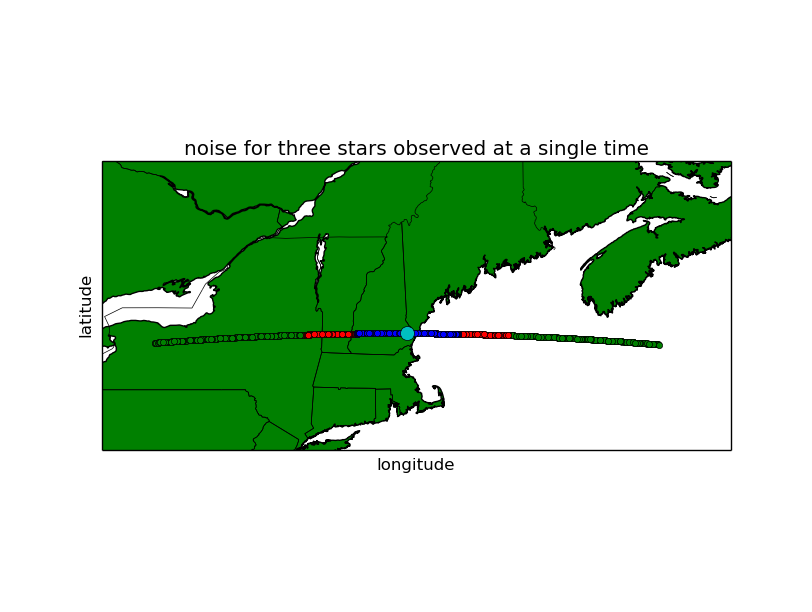
\includegraphics[height=10cm]{3s1t_single_total_noise.png}
\caption{Distribution of Estimates for Case 2 Observation Format: Uniform Noise Simulation}
\label{f:3s1t_single_total_noise}
\end{figure}

\begin{figure}[!htb]
\centering
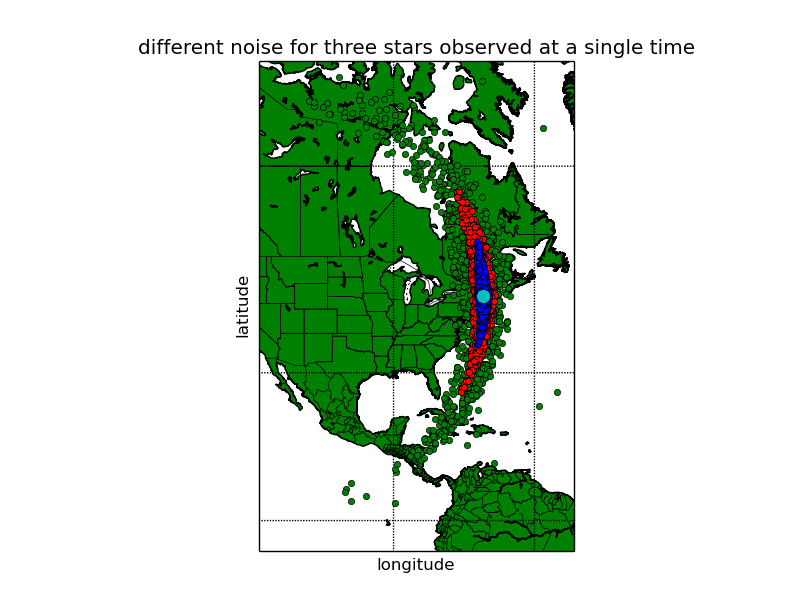
\includegraphics[height=10cm]{3s1t_single_case2_noise.png}
\caption{Distribution of Estimates for Case 2 Observation Format: Non-Uniform Noise Simulation}
\label{f:3s1t_case2_noise}
\end{figure}
\FloatBarrier
\subsection*{Case 3: One Star, Three Times}
Fig.~\ref{f:1s3t_case1_noise} depicts the Case 3 simulated observation with uniform noise.  
\begin{figure}[!htb]
\centering
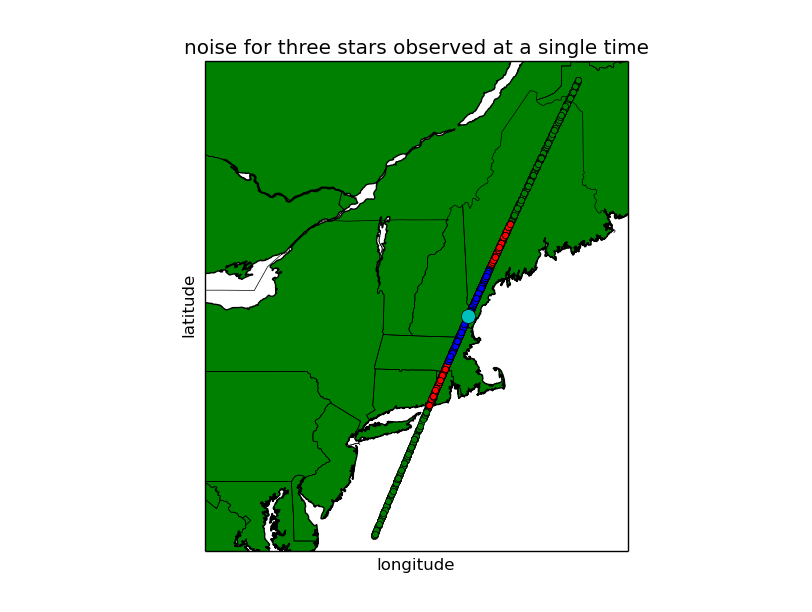
\includegraphics[height=10cm]{1s3t_case1_noise.png}
\caption{Distribution of Estimates for Case 3 Observation Format: Uniform Noise Simulation}
\label{f:1s3t_case1_noise}
\end{figure}
Fig.~\ref{f:1s3t_case2_noise} depicts the simulated observation of Case three with non-uniform noise.
\begin{figure}[!htb]
\centering
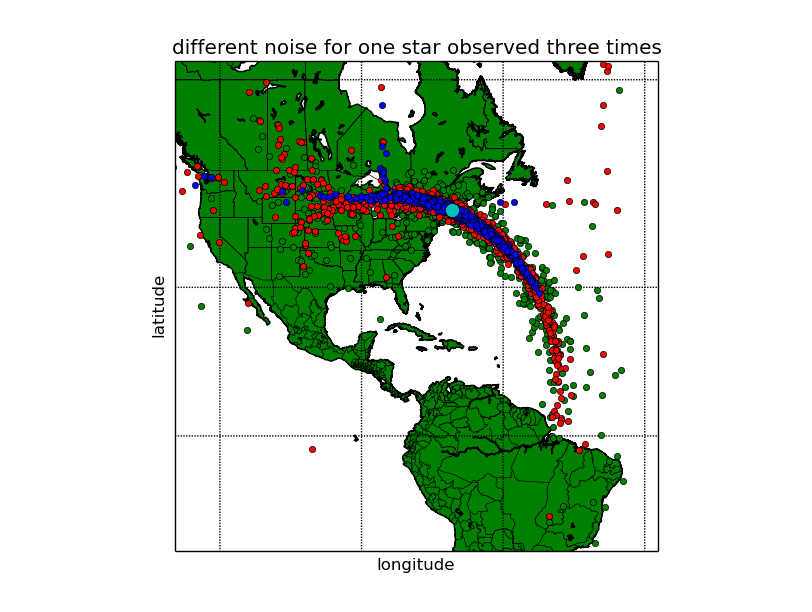
\includegraphics[height=10cm]{1s3t_case2_noise.png}
\caption{Distribution of Estimates for Case 3 Observation Format: Non-Uniform Noise Simulation }
\label{f:1s3t_case2_noise}
\end{figure}
Several values were not plotted because the predicted latitude and longitude were above the range of $(-180,180)$ for the longitude and $(-90, 90)$ for the latitude.  This meant that mean value was not an accurate predictor of location when one star was observed three times.  In addition, for points where the randomly generated bias in $H_{o}$ was high, the algorithm sometimes produced non-convergent results.  Case 3 is more sensitive to noise because it is only viewing one star, and the need for an accurate measurement is more pronounced.  For this observation format, the mean was not observed to be an accurate predictor of location.  Based on the above analysis, Case 3 was not selected for use on the star tracker.
\FloatBarrier
\section{Observation Bias}
Bias was artificially introduced into simulations to determine the effects of pitch offset.  Two cases were simulated.  In the first case, a uniform pitch offset (bias), $b_{i}$ is added to each of the three noisy star observations. In the second case, different biases are added to each of the three star observations. The key difference between this test and the previous noise tests, is that the values of bias added to the array of $H_{o,1}$, $H_{o,2}$, and $H_{o,3}$ are constant throughout each iteration of the simulation, and are not determined by a probability density function.  The array of observed altitudes describing the uniform bias test is shown in Eq.~(\ref{e:unibias}).
\begin{equation}
\begin{bmatrix}
H_{o,1,new} \\
H_{o,2,new}\\
H_{o,3,new}
\end{bmatrix} = 
\begin{bmatrix}
H_{o,1} + \epsilon_{1} + b_{1}\\
H_{o,2} + \epsilon_{2} + b_{1}\\
H_{o,3} + \epsilon_{3} + b_{1}
\end{bmatrix}
\label{e:unibias}
\end{equation}
The array of observed altitude describing the non-uniform bias test is shown in Eq.~(\ref{e:nunibias}).
\begin{equation}
\begin{bmatrix}
H_{o,1,new} \\
H_{o,2,new}\\
H_{o,3,new}
\end{bmatrix} = 
\begin{bmatrix}
H_{o,1} + \epsilon_{1} + b_{1}\\
H_{o,2} + \epsilon_{1} + b_{2}\\
H_{o,3} + \epsilon_{1} + b_{3}
\end{bmatrix}
\label{e:nunibias}
\end{equation}

\subsection*{Uniform Bias}
Fig.~\ref{f:biasShift} shows the distribution of uniformly biased, noisy observations from the Case 2 format. $b_{1}$ was set equal to $1^{\circ}$, $2^{\circ}$ and $5^{\circ}$ in this simulation.
\FloatBarrier
\begin{figure}[!htb]
\centering
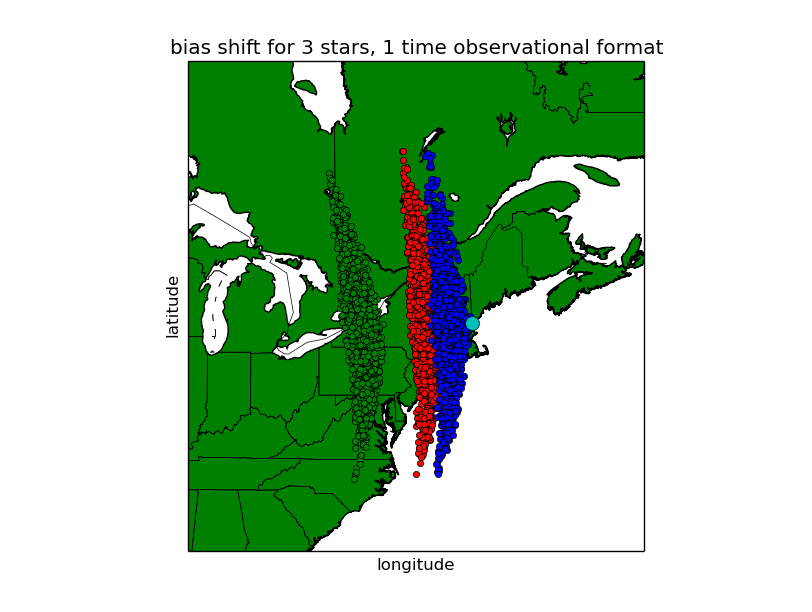
\includegraphics[height=8cm]{biasShift.png}
\caption{Uniform Bias Shift of Position Estimate}
\label{f:biasShift}
\end{figure}
\FloatBarrier Table~\ref{t:colorz3} shows the legend information for the Fig.~\ref{f:biasShift} simulations.
\begin{table}[ht!]
\centering
\begin{tabular}{ |c|c|c|c| } 
 \hline
 Blue & Red & Green & Teal\\ 
 \hline
 $b_{1} = 1^{\circ}$ & $b_{1} = 2^{\circ}$ & $b_{1} = 5^{\circ}$  & True Value \\ 
 \hline
\end{tabular}
\caption{Legend Format for Position Estimate Plots}
\label{t:colorz3}
\end{table}

Since the stars of Case 2 are very close together in the sky, and position determination is found by the intersection of three circles of equal altitude, it is currently believed that the distributions of points follow circles of equal altitude.  The direction of translation for the distribution may depend on the direction the stars were observed from.  Adding uniform bias to each $H_{o,i}$ in the observation vector is expected to alter the distribution of position estimates based on the orientation of the star camera.  Adding bias shifts the estimates towards the ground position of the star.  Subtracting bias moves the estimates away from the ground position of the star.  This is all observed in the figure and is consistent with comments from Blewitt regarding the size and behaviour of circles of equal altitude \cite{b:blewitt}. 
The mean points for the biased position estimates were examined for linear correlation to learn more about how the circles of positions change.  The estimated longitude is plotted against bias in Fig.~\ref{f:biasLon}.  The bias is observed to have a nearly linear response, with $R^{2}=0.99996$.  
\begin{figure}[!htb]
\centering
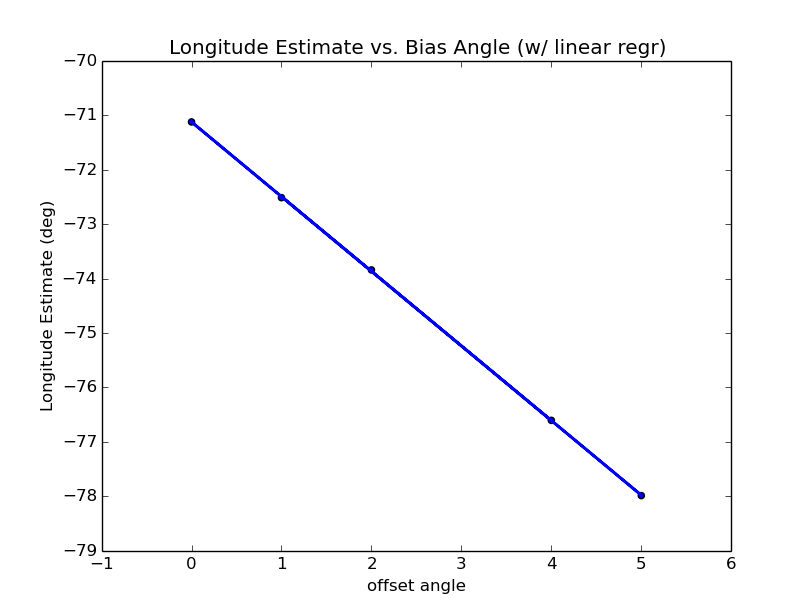
\includegraphics[height=8cm]{biasLon.png}
\caption{Longitude Estimate vs. Bias Shift}
\label{f:biasLon}
\end{figure}
The estimated latitude is plotted against bias in Fig.~\ref{f:biasLat}.  
\begin{figure}[!htb]
\centering
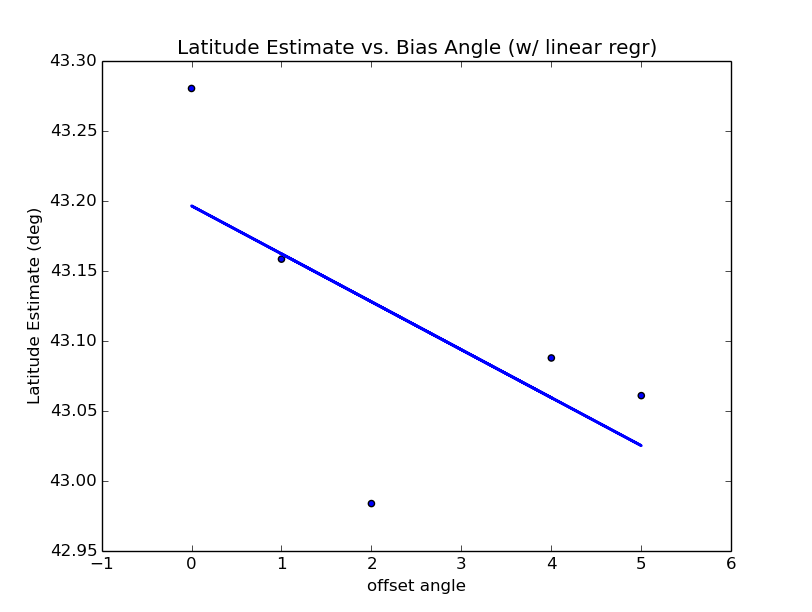
\includegraphics[height=8cm]{biasLat.png}
\caption{Latitude Estimate vs. Bias Shift}
\label{f:biasLat}
\end{figure}
In this case the linear model does not fit as well. The correlation coefficient was observed as $R^{2} = 0.40295$.  
\FloatBarrier
\subsection*{Non-Uniform Bias}
A short study was performed on the observations of Sulafat, Sheliak, and Vega to examine the effects of non-uniform bias.  Uniform noise of $\pm 1^{\circ}$ was added to each $H_{o,i}$ of the observation vector.  A bias of $+1^{\circ}$ was added to the observation of Sulafat. $+2^{\circ}$ was added to the observation of Sheliak.  $+5^{\circ}$ was added to the observation of Vega. The position estimates are depicted in Fig.~\ref{f:nonUniformBias}.
\FloatBarrier
\begin{figure}[!htb]
\centering
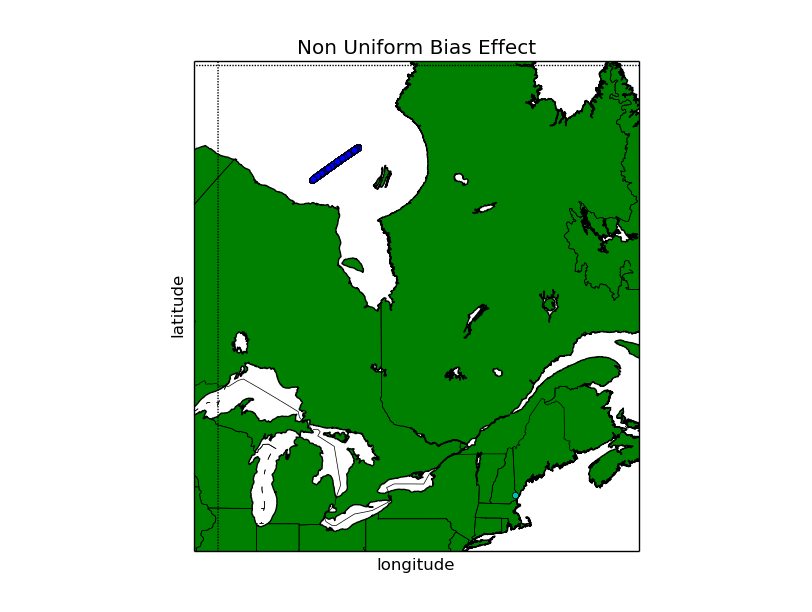
\includegraphics[height=8cm]{nonUniformBias.png}
\caption{Bias Study With Non-Uniform Bias Added to Sheliak, Sulafat, and Vega}
\label{f:nonUniformBias}
\end{figure}
\FloatBarrier
The estimated positions are observed to follow a line that has a different trajectory from those observed in the case of simple uniform noise injection. The position estimate is also less accurate.
\section{Summary of Observational Formats}
In summary, Case 2 was the best method simulated in order to obtain a viable position estimate.  The mean position estimate is a good indicator of the true position for uniform noise and low values of non-uniform noise.  The addition of uniform bias had a measurable effect on the dataset.  Case 2 requires only a single image to obtain a position estimate.
In addition to having the slowest number of iterations to convergence, Case 3 takes the longest to complete a single observation, since the camera shutter would need to be open for three times as long, and the orientation of the camera may have to change between images.  These difficulties of implementation makes for a suboptimal method of dynamic navigation.  Additionally, Case 3 has very little to no robustness to noise, or bias. This means that its application requires better sensors to function properly.  Since the geometric distribution of position estimates is non-uniform, the mean is not a good indicator of the position.  As such this method was not selected. Case 3 also requires three images to obtain a position estimate. 
Simulations of Case 1 led to an unexpected distribution of points. This unique distribution is likely caused by the varied locations of the observed stars in the night sky. Additionally, Case 1 requires three images to obtain a position estimate.  It may be viable for position determination after further study but ultimately was not selected for use in the experimental device.
Overall, each method is able to perform correct position determination given perfect sensors.  Based on the analysis of this section, the Case 2 observation format was selected for the experimental prototype.


%To test $\Gamma_{Total}$ some assumptions had to be made.  The first is a simplifying assumption, which is that all three accelerometers have the same orientation.  This means that $x_{1} = x_{2} = x_{3}$, $y_{1} = y_{2} = y_{3}$, and $z_{1} = z_{2} = z_{3}$, where the subscript indicates the accelerometer number.  For each test, each accelerometer the vector to be rotated is $[0, 0, 1]^{T}$.  Using these assumptions it is possible to test the equivalence of the three methods

%(((not too sure if i want to just leave this for future work or not)))
\chapter{Experimental Design and Verification}
This section details the hardware, software, and sources of error for the Celestial Navigation Device.  Different forms of error are disucssed.  Additionally, the experimental results are discussed, along with a generic calibration method which attempts to reduce the amount of error the device exhibits.
\section{Experimental Setup}
The experimental device is a Nikon D60 DSLR camera, with an attached Nikon 50mm f/1.8D Auto Focus Nikkor Lens. The D60 was chosen due to its charge coupled device (CCD) image sensor.  The CCD was believed to be important due to its linear response to light compared to a complimentary metal oxide semiconductor sensor (CMOS), which is the other leading type of image sensor found in digital cameras.  This factor was considered in the event that the image processing software would be manufactured in house.  It was later found that the response of CMOS and CCD sensors are both linear up to a saturation point \cite{b:cmos}.  This supports that CMOS cameras are also compatible with the star tracker design presented in this research.   The lens is set to the ``$\infty$" focus setting. The camera exposure time was eight seconds for each image, and the ISO sensor sensitivity was set to 800.  These settings were determined by trial and error to obtain a high quality image. A standard photography tripod is used to stabilize the camera housing along with a remote shutter to prevent movement from the user when the photograph of the stars is taken.  To ensure that adequate light is captured for star identification, the shutter remains open for 8 seconds per photograph. 
The camera flash attachment houses a Razor 9DOF inertial measurement unit (IMU).  The IMU reports the Euler angles between the local coordinate frame and the camera optical axis frame.  The IMU sets the Euler angles for the center pixel of the camera image.  Since useful navigational stars appear in locations other than the center pixel, an offset from the center pixel is applied using the field of view of the camera lens.  The camera setup has a field of view across the sensor diagonal of approximately 30.5 degrees.  This corresponds to an angular offset of approximately 24.2 arcseconds per pixel away from the center pixel.  These values for the field of view per pixel are calculated automatically in the Astrometry.net package and can also be calculated from the Pythagorean theorem.  The diagonal field of view of the D60 lens is $46^{\circ}$. The image is 3872Wx2592H pixels.  Trigonometry can be used to yield a factor of 24.1 arcseconds per pixel.  This fact is further confirmed by the Astrometry package. A laptop is used to record the local time and the IMU Euler angle output.  The setup is pictured in Fig.~\ref{f:setup}.

\begin{figure}[!ht]% order of placement preference: here, top, bottom
\centering
 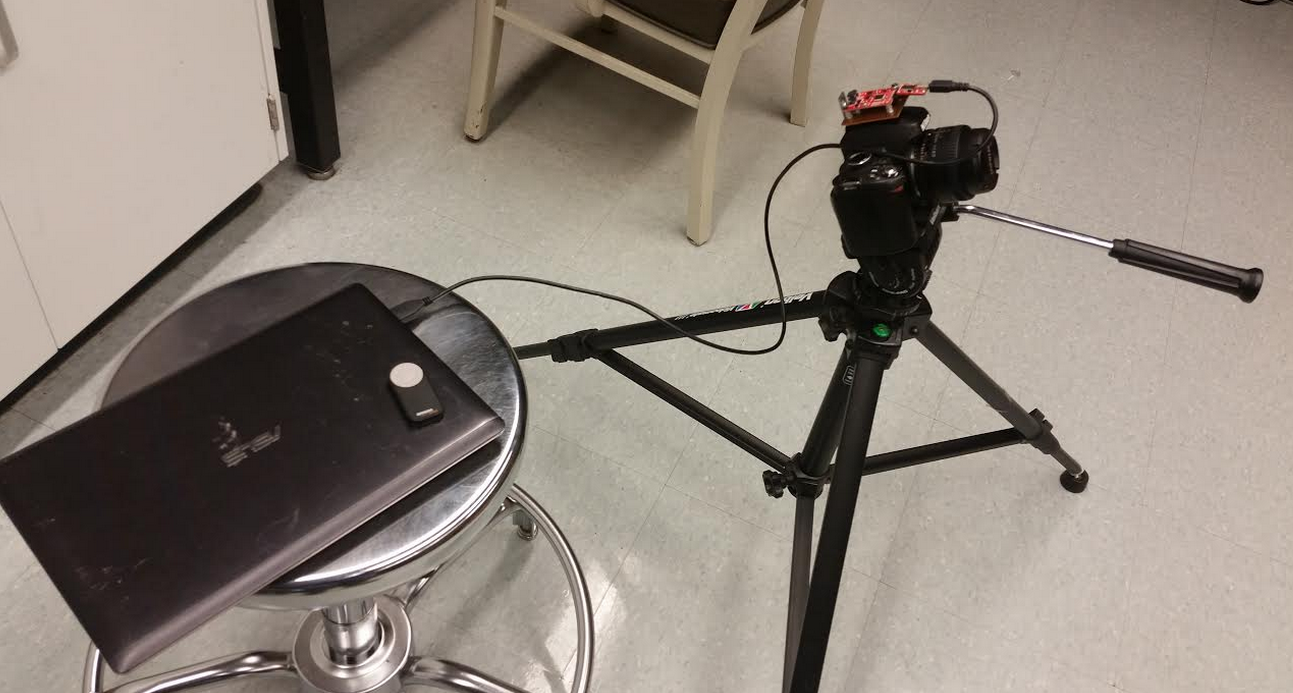
\includegraphics[width=10cm]{setup.png}
 \caption{Experimental setup for the Celestial Navigation Device.   The remote shutter can be seen on top of the laptop.}
 \label{f:setup}
\end{figure} 

\subsection{IMU Time Response Curves}
It was noted that while under USB configuration, the Razor 9-DOF IMU had a transient response.  This means that the pitch angle would changes over time after an initial warm up period. It is presently believed that this ``warm-up" time is a property of the IMU.  To avoid erroneous position estimation that is associated  with the IMU transient, the IMU is powered on for several minutes before measurements are taken.  A plot of the IMU pitch angle is shown in Fig.~\ref{f:manyPitchAngles} for several different initial conditions.
\begin{figure}[!ht]% order of placement preference: here, top, bottom
\centering
 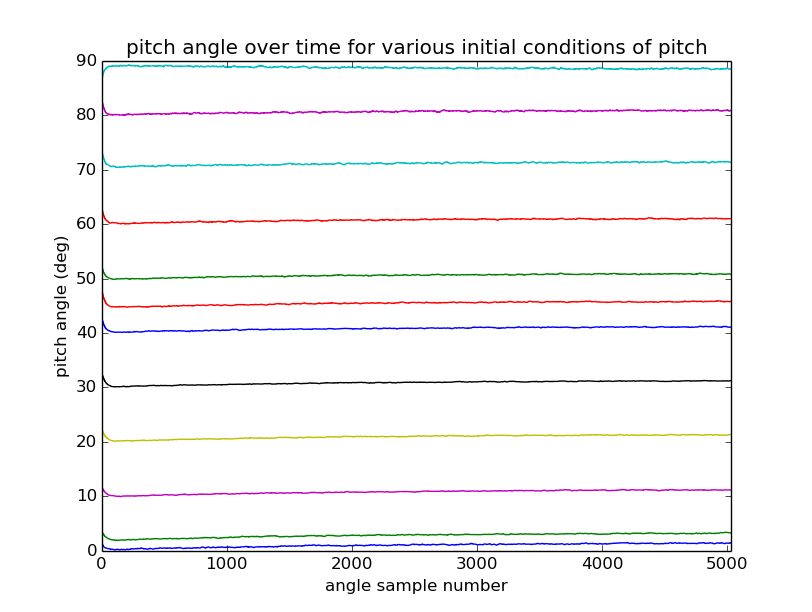
\includegraphics[width=10cm]{manyPitchAngles.png}
 \caption{Time response for various pitch angles.}
 \label{f:manyPitchAngles}
\end{figure} 
An interesting revelation of Fig.~\ref{f:manyPitchAngles} is that the 90 degrees trial has a first order response that is opposite in sign to the other nominal angle trials.  Computationally timing the data collection algorithm in a script estimated the sample rate to be 91.2Hz.  Two methods of processing are applied to the IMU pitch data according to the block diagram of Fig.~\ref{f:filterblock}. 
\begin{figure}[!ht]% order of placement preference: here, top, bottom
\centering
 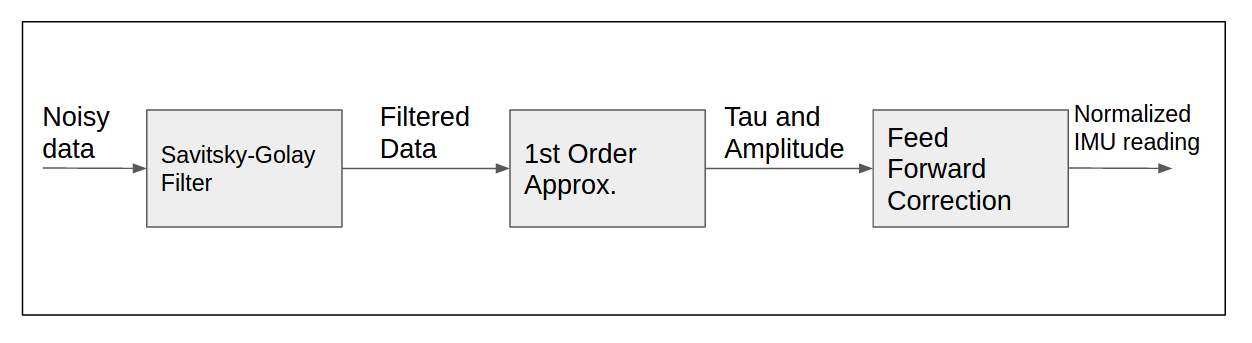
\includegraphics[height=4cm]{filterblock.png}
 \caption{Block Diagram for Filtering IMU data}
 \label{f:filterblock}
\end{figure} 
The first is a method known as Savitzky-Golay filtering.  This filtering mechanism is a digital filter which attempts to increase the signal to noise ratio by uses a moving window and fits different subsets of data to a different polynomial \cite{b:savgol}. Fig.~\ref{f:savgol} shows the results of Savitsky-Golay filtering.  Note that the angle is drifting to approximately 11 degrees, and that the vertical axis is expressed in scientific notation. The filtered data is the green data.
\begin{figure}[!ht]% order of placement preference: here, top, bottom
\centering
 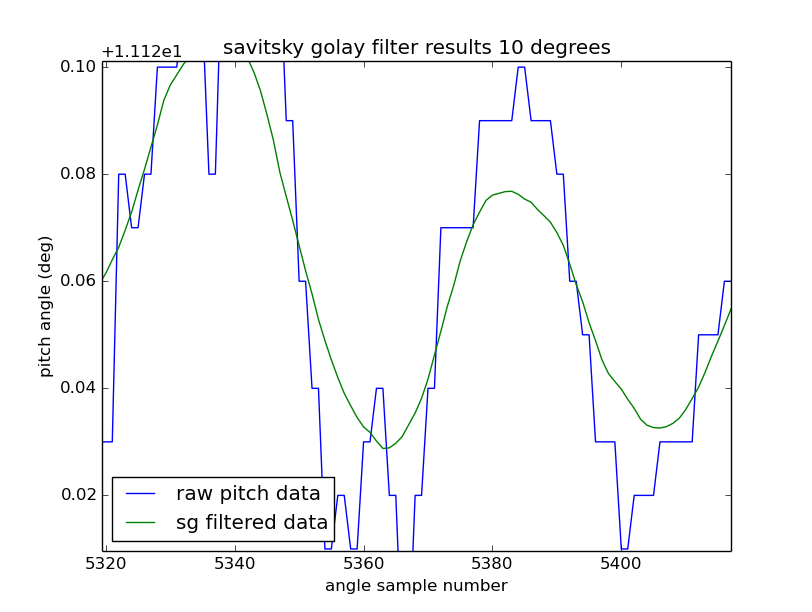
\includegraphics[width=10cm]{savgolay.png}
 \caption{Savistky-Golay Filtering.  }
 \label{f:savgol}
\end{figure} 
\FloatBarrier
It should be noted that while this filter does model the data more accurately, the pitch angle did not move for this experiment.  It is possible that the Savitsky-Golay filter may be attempting to model the noise.  For systems where a polynomial does represent the signal, Savitsky-Golay filtering may be optimal.  Further study into filtering methods for IMU transient response will need to be performed in order to achieve fully dynamic celestial navigation.

After filtering, a simple first order approximation is applied  \cite{b:ogata}.  A model of the form of Eq.~(\ref{e:1stOrder}) was applied. Where $A$ is the amplitude of the approximation, $t$ is time, and $\tau$ is a time constant that determines how quickly the system responds.  
\begin{equation}
x_{o}(t) = A(1-e^{\frac{t}{\tau}})
\label{e:1stOrder}
\end{equation}
Each trial of the nominal pitch was observed to show the first order behavior.  The model chosen to represent that behavior is shown in Eq.~\ref{e:firstorder1}
\begin{equation}
P(X) = P_{nominal} + A(1-e^{\frac{t}{\tau}})
\label{e:firstorder1}
\end{equation}

The model of Eq.~(\ref{e:firstorder1}) was performed on the IMU pitch measurements of Fig.~\ref{f:manyPitchAngles}.  An example of this approximation is shown in Fig.~\ref{f:firstorder} for nominal pitch of 10 degrees.  The IMU is seen to drift approximately 1.2015 degrees to 11.2015 degrees. $A$ was set equal to $1.2015$.   Using the 63.2\% method and the conversion listed above, the value of $\tau$ was found to be 24.557s.  This means that the IMU should rest for $4\tau$ or approximately 98.2 seconds uncompensated before attempting to read a new dynamic position.  This suggests that data will need to be processed to take into account time lag of the sensor if the camera is to be used in a dynamic application.

\begin{figure}[!ht]% order of placement preference: here, top, bottom
\centering
 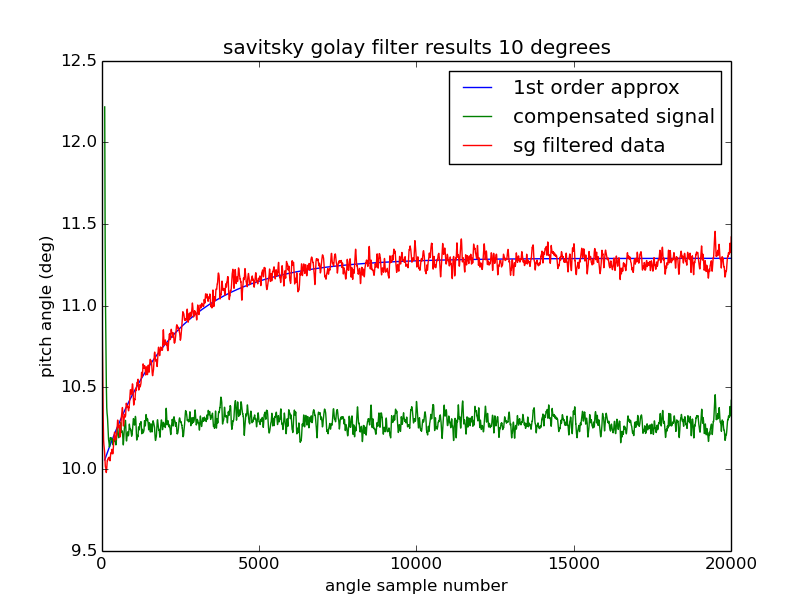
\includegraphics[width=10cm]{firstorder0.png}
 \caption{First Order Approximation of 10 degree pitch.}
 \label{f:firstorder}
\end{figure} 
Note that there is a strange transient that appears in approximately the first 100 samples.  This is likely the product of the moving average filter not having enough data across the initial samples. Further study is needed to see if this small transient signal will affect the celestial navigation camera in a dynamic setting. 

The IMU was powered on and collected 10000 pitch measurements while statically oriented at various pitch angles.  This test was performed to obtain the first order coefficients of  Eq.~(\ref{e:ffirstorder}). In this equation, $X$ represents the pitch measurement from the IMU, $\tau = 2253$ samples, $P(X)$ represents the pitch value as a function of sample $X$,  $P_{nominal}$ is the nominal pitch as measured from the filtered data.
\begin{equation}
P(X) = P_{nominal}+1.2915(1-e^{\frac{-X}{2253}})
\label{e:ffirstorder}
\end{equation}
In Fig.~\ref{f:firstorder}, $P_{nominal} = 10^{\circ}$.  This first order approximation was shown for the trials above to reduce a bias of approximately 1.3 degrees to approximately 0.2301 degrees. 

\section{Simulating Experimental Noise and Uncertainty Analysis}
It was desirable to determine the uncertainty of the observed estimate $H_{o}$ of the experimental star tracker.  Uncertainty levels for the candidate hardware were used in this calculation  \cite{b:imu}.  The uncertainty of a function, $q$, in multiple variables, $x, x_{1}, x_{2} ... x_{n}$ is determined by the Pythagorean sum of its partial derivatives multiplied by their respective uncertainties $\Delta x, \Delta x_{1}, \Delta x_{2} ... \Delta x_{n}$ \cite{b:uncertainty}.  

\begin{equation}
    \label{e:uncertain}
\Delta q = \sqrt{\left(\sum\limits_{i=1}^n  \frac{\partial q}{\partial x_{i}}\Delta x_{i} \right)^{2} }
\end{equation}
\\\\
Eq.~(\ref{e:uncertain}) was used in order to determine the uncertainty for the celestial navigation process.  A roll correction was derived.  This correction rolled the image pixel coordinates $x^{'}, y^{'}$ by an angle $\theta$.  This two dimensional rotation matrix is described in Eq.~(\ref{e:roll})
\begin{equation}
    \label{e:roll}
   \begin{bmatrix} 
  x     \\ 
  y 
\end{bmatrix}=\begin{bmatrix} 
  cos(\theta)     & -sin(\theta)\\ 
  sin(\theta) & cos(\theta) 
\end{bmatrix}\begin{bmatrix} 
  x^{'}\\ 
  y^{'} 
\end{bmatrix}
\end{equation}
Using Eq.~(\ref{e:uncertain}) normalized to determine the fractional uncertainty, the uncertainty for Eq.~(\ref{e:roll}), can be computed to be the following. 

\begin{equation}
\Delta y = \Delta x = \sqrt{\left(\Delta x^{'}\right)^{2} + \left(\Delta y^{'}\right)^{2} + \left(\Delta \theta\right)^{2}}
\end{equation}
Application of Eq.~(\ref{e:uncertain}) leads to the full uncertainty equation of Eq.(\ref{e:sumdelta}).
\begin{equation}
    \label{e:sumdelta}
\Delta H_{o} = \sqrt{ 2\left(\Delta x^{'}\right)^{2} + 2\left(\Delta y^{'}\right)^{2} +2\left(\Delta \theta\right)^{2} +\left(\Delta \phi\right)^{2}   }
\end{equation}

Using Eq.(\ref{e:sumdelta}), $\Delta x = \Delta y = 24.2$ arcseconds, $\Delta \theta = \Delta \phi = 0.1^{\circ}$, the approximate uncertainty was found to be 600 arcseconds. This is only one-sixth of one degree. The scatter plot of position estimates given an assumed location of Durham, NH is presented below in Fig.~\ref{f:map2222}
\begin{figure}[!h]
\centering
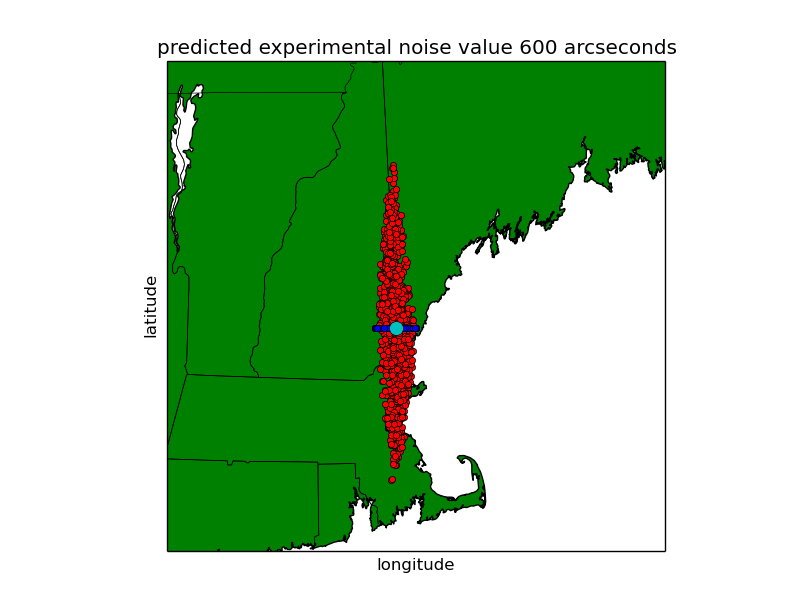
\includegraphics[height=8cm]{map2222.png}
\caption{Position estimates with 600 arcseconds of uncertainty. Teal represents the true value, Blue is the position estimates with uniform noise, and red is the position estimate with non-uniform noise.}
\label{f:map2222}
\end{figure}

%\section{$\Gamma$ Matrix Comparison}
%This section compares the output of different methods for calculating the body to local coordinate transformation $\Gamma$.  The first method, $\Gamma_{Total}$ is one that uses three three axis accelerometers.  The second method, $\Gamma_{EXP}$ uses a simple altitude and azimuth rotation to determine the rotation, and is principally theoretical in nature.  The third method, $\Gamma_{Phone}$, is the method used by smartphone accelerometers to determine orientation. 
\section{Experimental Software}
The software for the experiment is written in Python 2.7 and can be cloned for personal use from the github.com repository ``https://github.com/ckflight/unh-startracker".  The Python scripts consist of three major components, each corresponding to the three major components of Fig.~\ref{f:diagram}.  A block diagram of this software is depicted in Fig.~\ref{f:software}.  Part A of the block diagram depicts the system block diagram.  Part B of the block diagram indicates the experimental and software implementation of the system.
\begin{figure}[!ht]% order of placement preference: here, top, bottom
\centering
 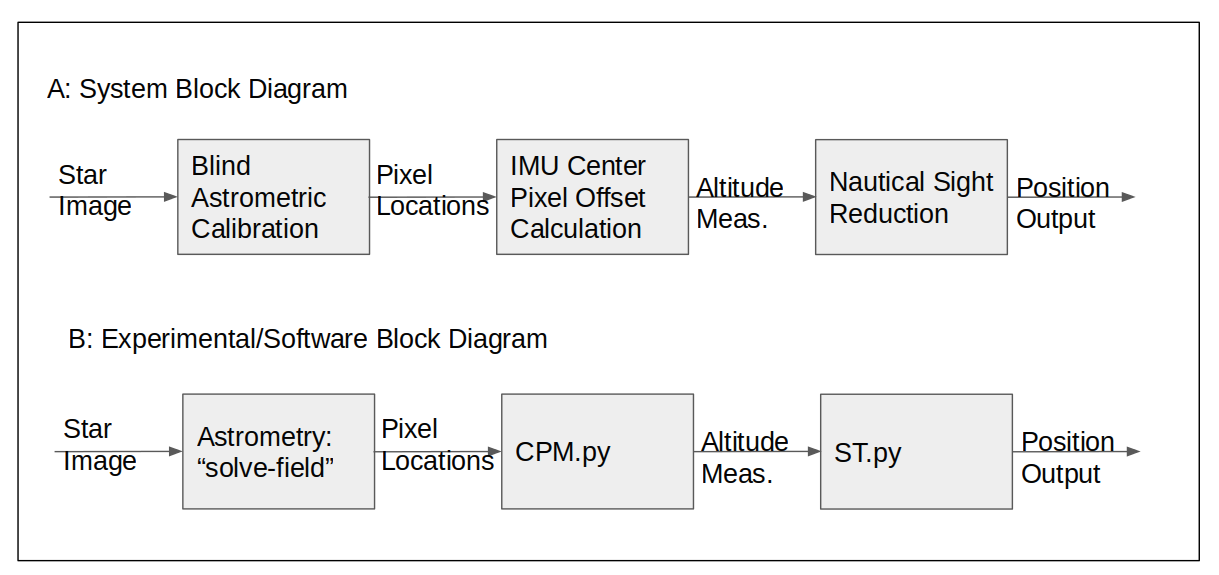
\includegraphics[height=4.5cm]{software.png}
 \caption{Software Block Diagram for Nautical Sight Reduction.}
\label{f:software}
\end{figure} 
The first piece, ``Astrometry" is described in detail in the next subsection. Its main purpose is locating stars of interest in the image.  It outputs data about the stars, or ``sources" in a data dictionary where they can be accessed by another program. In this case, the pixel locations from the data dictionaries are read by CPM.py.  CPM.py is a script that performs the center pixel method, determining star locations relative to the image center pixel and converting star image location into an observed altitude.  CPM.py also provides other important features such as the capability to run Astrometry ``solve-field" either from the Astrometry.net online server or on a personal computer.  Astrometry.net ``solve-field" is the command line version of this program capable of identifying sources in the input images.  Running ``solve-field" from a personal computer is much faster.  The primary advantage of using the online server is that it displays a result image containing labels of the sources and circles around the sources found in the image.  This is very useful for diagnostic purposes.  CPM.py also performs basic tasks such as unit conversion and extracting the time a photo was taken from each image file   and forwarding it to the next program.  

ST.py takes the attitude measurement provided by CPM.py and performs the Nautical Sight Reduction method as described in Chapter 2. ST.py also provides all the math functions used by itself and CPM.py, such as trigonometric functions that take arguments expressed in degrees.  Most importantly, ST.py provides a function by which CPM.py can express the y-coordinate of a source star in rectangular or spherical gnomonic projected coordinates.  A script known as starmap.py is used to display the maps and histograms of the data.  These scripts are available in the Appendices.  
\subsection{Blind Astrometric Calibration}
The Astrometry.net software was written by Lang et. al.  \cite{b:astro}.  The main idea behind the software is to take astronomical photographs and identify astronomical objects, termed ``sources" in a generalized lost in space case. Solving the lost in space case means that the stars can be identified simply by their image, and no other input data is necessary. Therefore, the Astrometry.net software uses only data stored in the image pixels, and does not use any metadata such as the size of the image.  Source extraction and identification are performed in two parts.  The first part, termed "the easy part" by the original authors, is locating the sources in the image.  This is performed by an algorithm called SExtractor.  This algorithm processes the image to determine a noise level $\sigma$ and identifies objects who exceed that noise level by $8\sigma$.  Further processing is performed to find the centroids of these objects by a Guassian fit.  Brightness, from center to edge of the star image typically follows a a Gaussian fit.  The results of this process are shown in Fig.~\ref{f:centroids}.
\begin{figure}[!ht]% order of placement preference: here, top, bottom
\centering
 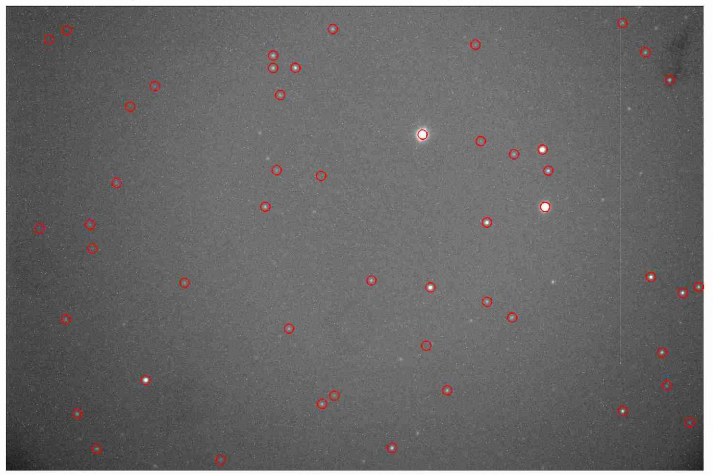
\includegraphics[width=10cm]{centroids.png}
 \caption{Centroid Output of Astrometry.net Software}
\label{f:centroids}
\end{figure} 
\FloatBarrier
The next part, termed ``the hard part" by the original authors is similar to the method described by Pyramid-LISA, in that ``pyramids", or combinations of four stars, are identified in the image.  Pyramids are then compared to a catalog of stars, in this case the catalog used in the USNO-B catalog of stars.  This catalog from the U.S. Naval Observatory is suitable for navigation because it catalogs the entire sky to an accuracy of 0.2 arcseconds ($5.5(10^{-5})$ degrees).   An example of the pyramids found by the program are shown in Fig.~\ref{f:pyramids}.  
\begin{figure}[!ht]% order of placement preference: here, top, bottom
\centering
 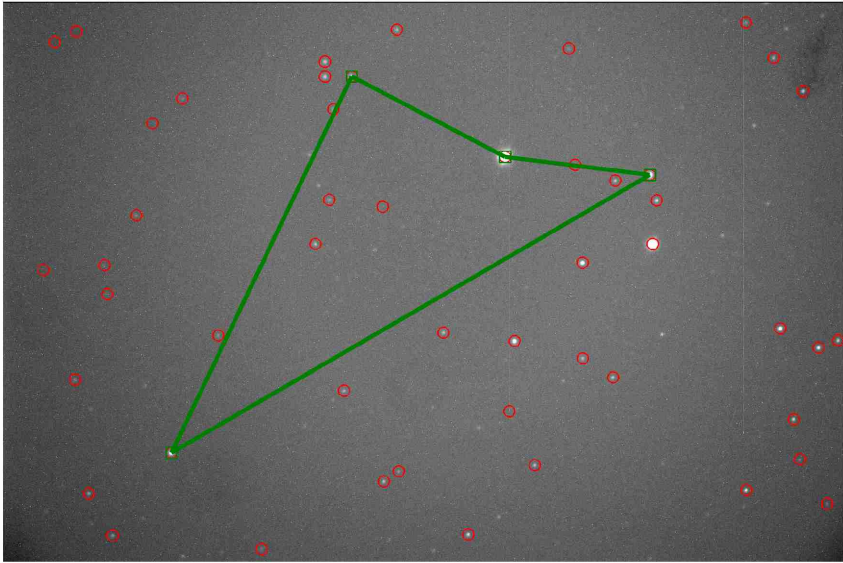
\includegraphics[width=8cm]{pyramids.png}
 \caption{``Pyramid" Output of Astrometry.net Software}
\label{f:pyramids}
\end{figure} 

The key feature of Astrometry, and what makes it the premier software of its kind is that it uses only a single pyramid to determine the starfield in the image.  A hash table of the USNO-B catalog is precomputed for use by the algorithm.  From there, a hash of the brightest pyramid in the image is compared to the table of hashes to determine where in the celestial sphere the image is taken.  The underlying mechanics, such as the actual hash table development, and the Bayesian statistical model by which a determination of which stars are identified by the quad, are beyond the scope of this research and can be found in the literature \cite{b:lang2}.  
\subsection{Small Angle Approximation}
The experimental results provided in this thesis all rely on the small angle approximation such that:
\begin{equation}
sin(\theta) \approx \theta
\end{equation}
\begin{equation}
cos(\theta) \approx 1 - \frac{\theta^{2}}{2}
\end{equation}
\begin{equation}
tan(\theta) \approx \theta
\end{equation}
Plots of this approximation are shown below in Fig.~\ref{f:smallAngle} and Fig.~\ref{f:smallAngleO}
\begin{figure}[!ht]% order of placement preference: here, top, bottom
\centering
 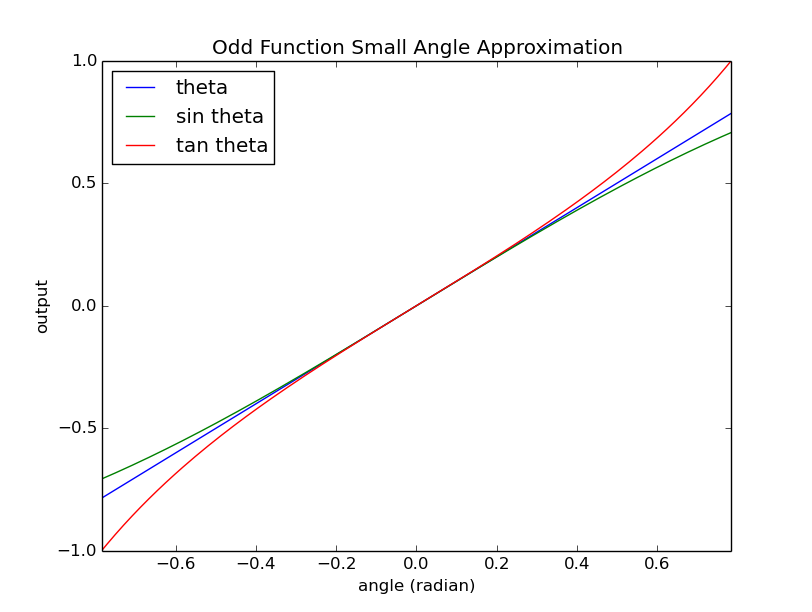
\includegraphics[width=10cm]{smallAngle.png}
 \caption{Small Angle Approximation of Odd Trigonometric Functions for $\{\theta \in \mathbb{R} \vert -\frac{\pi}{4} < x < \frac{\pi}{4}\}$}
\label{f:smallAngle}
\end{figure} 
\begin{figure}[!ht]% order of placement preference: here, top, bottom
\centering
 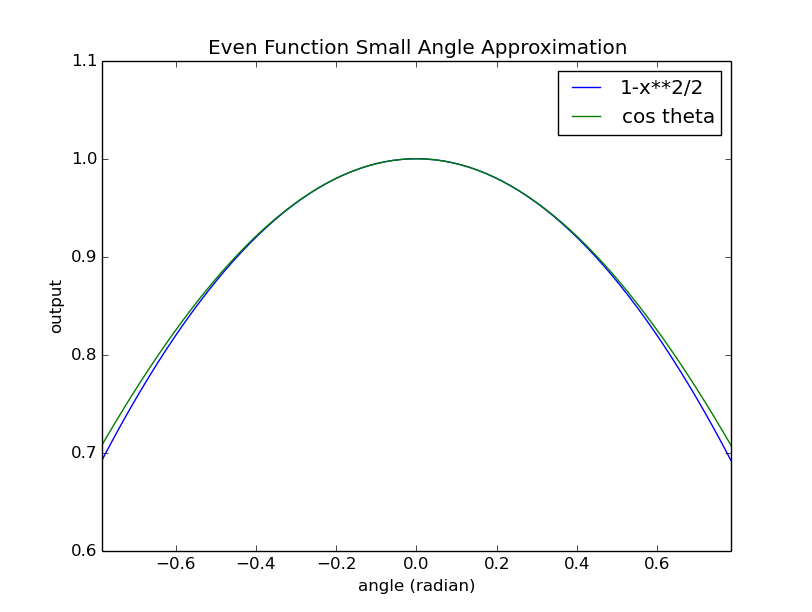
\includegraphics[width=10cm]{smallAngleO.png}
 \caption{Small Angle Approximation of Even Trigonometric Functions for $\{\theta \in \mathbb{R} \vert -\frac{\pi}{4} < x < \frac{\pi}{4}\}$}
\label{f:smallAngleO}
\end{figure} 
A plot of the absolute relative error is shown in Fig.~\ref{f:absrel}.
\begin{figure}[!ht]% order of placement preference: here, top, bottom
\centering
 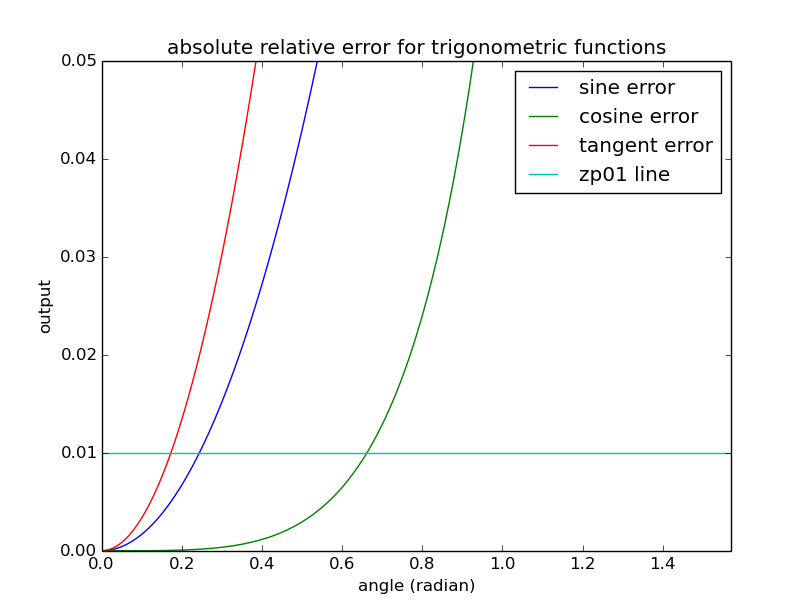
\includegraphics[width=10cm]{trigabsrel.png}
 \caption{Absolute Relative Error with bounding 1\% line for Sine, Cosine, and Tangent Functions}
\label{f:absrel}
\end{figure} 
\FloatBarrier
A threshold of 1\% error was arbitrarily selected in order to ensure that data collected from the star tracker can be input to linear translation and rotation representations for optimization.  Since the smallest angle that can be used corresponds to the approximation of the sine function, the maximum angle used in future star tracker datasets was approximately 9.75 degrees.  This angular constraint requires that the star observations are closer than 725 pixels to the center pixel.  This radius is drawn onto a sample image in Fig.~\ref{f:maxradius}.
\begin{figure}[!ht]% order of placement preference: here, top, bottom
\centering
 \includegraphics[height=10cm]{maxradius.png}
 \caption{1\% Small Angle Approximation Circle for example astronomical photograph}
\label{f:maxradius}
\end{figure} 
\FloatBarrier
Section 4.4.1 will detail the possible use of the spherical gnomonic projection which seeks to eliminate the need for the small angle approximation.  

\section{Experimental Results}
The Nautical Sight Reduction Algorithm was performed on experimental images.  Using Astrometry, altitude measurements of star centers were obtained.  These measurements were taken from Durham, New Hampshire.  With no correction for roll, the mean estimated point is 78.2927W, 44.2405N.  The true point is 70.9349W, 43.1337N.  This resulted in a mean error of 382.9 nautical miles and can be seen in Figure~\ref{f:nomods}. It can be seen from the data that the distribution of points follows a trend similar to those suggested by the uniform noise distribution of Chapter 3. 
\FloatBarrier
\begin{table}[ht!]
\centering
\begin{tabular}{ |c|c|c|c|c| } 
 \hline
 $P_{off}$ & $\theta_{off}$ & Latitude Est.($\circ$) & Longitude Est.($\circ$)&Error ($\circ$) \\ 
 \hline
 $0$ & $0$ & $-78.2927$ & $44.2405$ &$7.4405$   \\ 
 \hline
\end{tabular}
\caption{Results for Unbiased Nautical Sight Reduction Algorithm}
\label{t:nomods}
\end{table}
\begin{figure}[!ht]
\centering
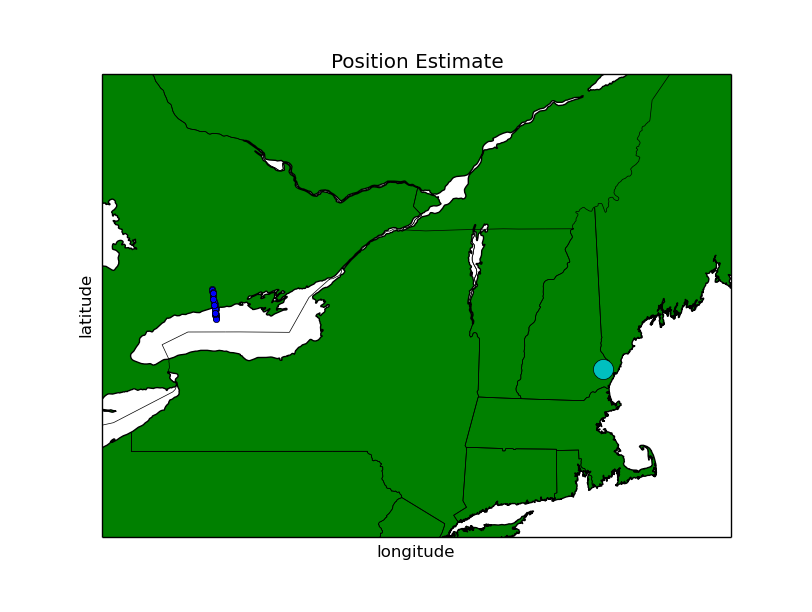
\includegraphics[height=8cm]{nomods.png}
\caption{Star Camera error with no modifications}
\label{f:nomods}
\end{figure}
\FloatBarrier
A modification of the pitch measurement based on calibration images was added in order to help obtain a more accurate result.  This modification is designed to be close to the unmodeled pitch bias.  The calibration  method attempted to observe a star in the image center pixel and compare $H_{o}$ and $H_{c}$ from Eq.~(\ref{e:p}) to determine the bias values. The pitch offset value was -5.109 degrees. The negative sign corresponds to the IMU being pitched too high. The mean estimated point was 71.0236W, 44.2956N.  The mean error was 77.09 nautical miles.  Error can be observed in the latitude as time increases.  This can be seen in Figure~\ref{f:pitched_map}.  These results are summarized in Table~\ref{t:pitched}
\FloatBarrier
\begin{figure}[!ht]
\centering
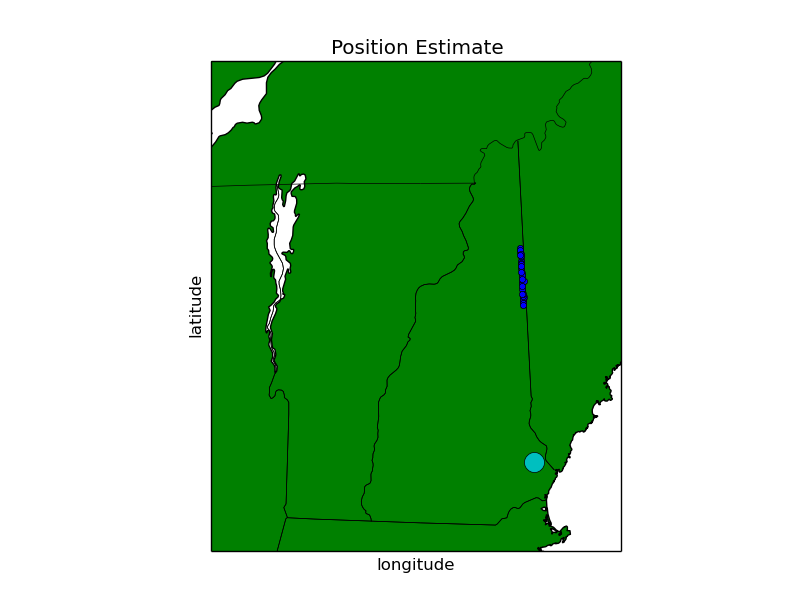
\includegraphics[height=8cm]{pitched_map.png}
\caption{Star Camera error with pitch modification}
\label{f:pitched_map}
\end{figure}

\begin{table}[ht!]
\centering
\begin{tabular}{ |c|c|c|c|c| } 
 \hline
 $P_{off}$ & $\theta_{off}$ & Latitude Est.($\circ$) & Longitude Est.($\circ$)&Error ($\circ$) \\ 
 \hline
 $-5.109$ & $0$ & $-71.0236$ & $44.2956$ &$1.156$   \\ 
 \hline
\end{tabular}
\caption{Simple Pitch Compensation for Rectangular Coordinate Center Pixel Method Cost Function}
\label{t:pitched}
\end{table}
\FloatBarrier

Arbitrary calibrations of the roll offset led to a more accurate result.  An offset of $-2^{\circ}$ was arbitrarily applied in the roll axis of a sample image.  The results are shown in Fig.~\ref{f:rollmod}, indicating a mean error of approximately 4.5 nautical miles.  It was qualitatively apparent that finding a correct roll offset minimizes position estimate error.  The method by which roll offset is determined is presented in the following section.  
\begin{figure}[!ht]
\centering
\includegraphics[height=8cm]{rollmod.png}
\caption{Star Camera error with arbitrary roll modification}
\label{f:rollmod}
\end{figure}
\FloatBarrier
\section{Optimization Techniques for Generic Calibration}
Pitch and roll offsets cause error in the star camera method.  Quantifying these offsets serves to reduce this error.  Eq.(\ref{e:cost}) shows the cost function that modeled error as a function of pitch offset, $P_{off}$ and roll offset $\theta_{off}$.  
\begin{equation}
    \label{e:cost}
J = \sum\limits_{i=1}^n  \Big(x_{i}\sin(\theta_{imu} + \theta_{off}) + (y_{i} + P_{imu} + P_{off})\cos(\theta_{imu} + \theta_{off})-(H_{c})_{i}\Big)^{2}
\end{equation}
This equation was derived by first translating the initial y-coordinate of the star, $y_{i}$ by $P_{off}$ for each sample $n$.  Then, the star is rolled in the image by $\theta_{off}$. $x_{i}$ is the initial x-coordinate of the star.  $P_{imu}$ and $\theta_{imu}$ are the measured IMU pitch and roll, respectively.  Finally, $(H_{c})_{i}$ is the computed altitude of the star, determined by Eq.(\ref{e:Hc}).   It should be noted that the units of the coefficient terms are in pixels.  The units of the argument terms are in degrees.

The cost function of a single observation was plotted in Fig.~\ref{f:singleCost} to examine its qualitative properties.  
\begin{figure}[!ht]
\centering
\includegraphics[height=8cm]{singleCost.png}
\caption{Cost Function of a Single Observation}\label{f:singleCost}
\end{figure}
It can be observed that along the roll axis, the behavior is periodic.  This is expected because the roll offset is based on a rotation.  Every $360^{\circ}$ the trend in the roll repeats itself.  On the pitch axis, the error is high for large offsets. Then, as the pitch approaches the true altitude, the error reaches some minimum and increases again as the pitch begins to overshoot.  This is an expected result since the plane of the image is currently modeled as Cartesian space.  It follows logically that the sum of the cost functions for each observation, depicted in Fig.~\ref{f:sumCost}, follows the same trends.   Note the higher multiplier on the z-axis.
\begin{figure}[!ht]
\centering
\includegraphics[height=8cm]{sumCost.png}
\caption{Cost Function for entire Lyra Constellation Dataset.}\label{f:sumCost}
\end{figure}
\FloatBarrier
An optimization method was tested to minimize the cost function and characterize the pitch and roll offset. The bounds of the search space are $\pm 15^{\circ}$.  These bounds are fairly lenient and are used to show that lumped error correction is a possibility.  Errors above a certain threshold could be from IMU misalignment or poor craftsmanship in the construction.  For a production quality star tracker, the optimization would be performed in software after the aforementioned processes were fine tuned.  The method used is a parameter space sample and search. This method is simple to implement and determines the minimum value, but is very inefficient because it has to check every element of the resulting matrix. %The second was Particle Swarm Algorithm, which uses multiple agents, random number generation, and distributed control to determine a global minimum.
\subsection*{Parameter Space Search}
This algorithm is very simple, at the expense of being very computationally intense.  First, an $m \times n$ matrix is computed, where $m$ and $n$ represent the number of elements in each dimension of the parameter space.  Then, the function is evaluated at each of those predefined points and placed into an array.  Each element of the array is then iterated over in order to find the minimum value.  A script was written in MATLAB to perform this task.  The optimization is performed by the following function.

\begin{verbatim}
[r,c] = find(J==min(min(J)))
\end{verbatim}
In this function, J represents the cost function matrix. \verb|Find| and \verb|min| are MATLAB functions that find the indices of a matrix based on certain criteria.  In this case they are used to find the minimum value.    
For a grid of 1000 points that were defined from $\pm 15^{\circ}$ the results found are depicted in Table~\ref{t:parameterSearch}.  This arrangement of points allows a resolution of $0.03^{\circ}$.  The results of this table depict an angular error of approximately $1.268^{\circ}$ 

\begin{table}[ht!]
\centering
\begin{tabular}{ |c|c|c|c|c| } 
 \hline
 $P_{off}$ & $\theta_{off}$ & Latitude Est.($\circ$) & Longitude Est.($\circ$)&Error ($\circ$) \\ 
 \hline
 $-4.9399$ & $-4.7598$ & $-70.634$ & $41.901$ &$1.268$   \\ 
 \hline
\end{tabular}
\caption{Optimal Pitch and Roll for Rectangular Coordinate Center Pixel Method Cost Function}
\label{t:parameterSearch}
\end{table}

The position estimates of sighting of the constellation Lyra on October $9^{th}$, 2015 with the optimal roll and pitch added to the calculation result in the map of Fig.~\ref{f:optimalRectangular}.  Notable here is that despite the algorithm being apparently well optimized when examined in terms of degrees, even the $1.268^{\circ}$ error found in this method translate into approximately 75 nautical miles of error.

\begin{figure}[!ht]
\centering
\includegraphics[height=10cm]{optimalRectangular.png}
\caption{Map of Position Estimate Output With Rectangular Center Pixel Method}\label{f:optimalRectangular}
\end{figure}
\FloatBarrier
The heading of this error is noted to be the opposite direction of the test where only the pitch offset was modified.  It appears that the roll of the IMU has the greatest effect on the estimate of the latitude.  Taking the mean of the estimates calculated by adjusting only the pitch offset and then by adjusting the roll offset gives an improved result depicted in Table \ref{t:rectMeanEstimate}.  The result was an error of approximately 5 nautical miles.    The position given by this optimization is shown in Fig.~\ref{f:rectMeanEst_map}.  
\begin{table}[ht!]
\centering
\begin{tabular}{ |c|c|c|c|c| } 
 \hline
 $P_{off}$ & $\theta_{off}$ & Latitude Est.($\circ$) & Longitude Est.($\circ$)&Error ($\circ$) \\ 
 \hline
 $n/a$ & $n/a$ & $-70.8226$ & $43.147$ &$0.1177$   \\ 
 \hline
\end{tabular}
\caption{Mean Position Estimate Tabular Results}
\label{t:rectMeanEstimate}
\end{table}
\begin{figure}[!ht]
\centering
\includegraphics[height=10cm]{rectMeanEst_map.png}
\caption{Map of Mean Position Estimate Output With Rectangular Center Pixel Method}\label{f:rectMeanEst_map}
\end{figure}



A slightly improved result is obtained by first optimizing the pitch angle with no roll then optimizing the cost function for pitch and roll, and taking the mean of the two output parameters.  The results of this process are shown in Table~\ref{t:rectMeanParams}.  The error of $0.0586^{\circ}$ is promising, and is only approximately 3 nautical miles of error.  The map of this estimation is shown in Fiq.~\ref{f:rectMeanParams_map}.  
\begin{table}[ht!]
\centering
\begin{tabular}{ |c|c|c|c|c| } 
 \hline
 $P_{off}$ & $\theta_{off}$ & Latitude Est.($\circ$) & Longitude Est.($\circ$)&Error ($\circ$) \\ 
 \hline
 $-5.0244$ & $-2.3799$ & $-70.8769$ & $43.1420$ &$0.0586$   \\ 
 \hline
\end{tabular}
\caption{Optimal Pitch and Roll for Rectangular Coordinate Center Pixel Method Cost Function}
\label{t:rectMeanParams}
\end{table}

\begin{figure}[!ht]
\centering
\includegraphics[height=10cm]{rectMeanParams_map.png}
\caption{Map of Position Estimate Output With Rectangular Center Pixel Method Mean Parameters Method}\label{f:rectMeanParams_map}
\end{figure}
For further visualization, the mean estimated point is plotted along with the real point on Google Maps, Fig.~\ref{f:cool}. Note that the red pin is the estimated point and the white circle is the true location.    

\begin{figure}[!ht]
\centering
\includegraphics[height=6cm]{cool.png}
\caption{Google Map Visualization of Position Estimate Output With Rectangular Center Pixel Method Mean Parameters Method}\label{f:cool}
\end{figure}
\FloatBarrier

\subsection{Optimizing Time Invariant Error}
One form of time invariant error is suspected to originate from the requirement that the Celestial Navigation Device adhere to the small angle approximation.  The current experimentally implemented version of the center pixel method uses a rectangular approximation.  This approximation works best for astrophotography applications with small fields of view.  In the case of this celestial navigation device, the field of view is over 30 degrees.  The small angle approximation dictates that only a small area of the image be used for legitimate observations.  Recall the equations for the small angle approximation from the previous section.  
One method attempted to refine the time invariant error is the gnomonic projection \cite{b:gnomonic}.  This method is expected to aid both the time invariant error and the time varying error because it will eliminate the need to use stars close to the center pixel.  Currently, the stars in the observation are selected to be as close to the center pixel as possible in order to adhere to the small angle approximation.  The gnomonic projection seeks to eliminate the need for this proximity is described below.  The gnomonic coordinate transformation is essential because the light from the star passes through a spherical lens, onto a CCD element, a flat plane.  An example of this distortion can be seen in Fig.~\ref{f:gp} \cite{b:gnomonic}.
\begin{figure}[!ht]
\centering
\includegraphics[height=6cm]{GP.jpg}
\caption{Gnomonic Projection Distortion \cite{b:gnomphoto}}\label{f:gp}
\end{figure}
The relationship between the spherical and planar coordinate frames is given as follows. The center points of the gnomonic projection are $\phi_{1}$ and $\lambda_{0}$ for the horizontal and vertical coordinates, respectively.  $\phi$ represents the horizontal coordinate, and $\lambda$ represents the vertical coordinate.  
\begin{equation}
\phi = sin^{-1} \left ( cos(c)sin(\phi_{1}) + \frac{ysin(c)cos(\phi_{1})}{\rho}\right)
\end{equation}

\begin{equation}
\lambda = \lambda_{0} + tan^{-1}\left (\frac{xsin(c)}{\rho cos(\phi_{1}) cos(c) - y sin(\phi_{1})sin(c)}\right)
\label{e:lambda}
\end{equation}
\begin{equation}
\rho = \sqrt{x^{2} + y^{2}}
\end{equation}
\begin{equation}
c = tan^{-1}(\rho)
\end{equation}

The gnomonic projection modifies the y-coordinate $y_{i}$ of Eq.~(\ref{e:cost}) to the value $Y_{i}$ of Eq.~(\ref{e:costGnom}). In Eq.~(\ref{e:costGnom}), $Y_{i}$ is calculated according to the gnomonic projection equations. The value of $\lambda_{0}$ in Eq.~(\ref{e:lambda}) is defined by the IMU measurement $P_{imu}$.  The horizontal initial coordinate $\phi_{1}$ is set equal to zero. A figure of this new cost function is depicted in Fig.~\ref{f:gnomCost}.  
\begin{figure}[!ht]
\centering
\includegraphics[height=8cm]{gnomCost.png}
\caption{Gnomonic Projection Cost Function}\label{f:gnomCost}
\end{figure}
The gnomonic projection cost function exhibits the same trends as the rectangular projection.  It was observed that the maximum value of error was less than the maximum value predicted in the rectangular cost function. The observed values for the sum squared error is $4.924(10^{11})$ for the rectangular cost function compared to $4.908(10^{11})$ for the gnomonic cost function.  It was later observed that the optimal point for the gnomonic projection led to higher overall error.
\begin{equation}
    \label{e:costGnom}
J = \sum\limits_{i=1}^n  \Big(x_{i}\sin(\theta_{imu} + \theta_{off}) + Y_{i}\cos(\theta_{imu} + \theta_{off})-(H_{c})_{i}\Big)^{2}
\end{equation}
The experimental observation with a value of $P_{off} = 0$, and $\theta_{off} = 0$ is depicted in Fig.~\ref{f:gnomRaw_map}.  The results are summarized in Table~\ref{t:gnomRaw}.  It can be seen that the gnomonic projection actually increases the error compared to that of the rectangular approximation.  This is unfortunate and likely points to a mistake in the implementation rather than a flaw in the established theory.  This method of estimation led to an error of approximately 799 nautical miles.  This is about two times the error from the rectangular method, and does not seem to indicate usefulness for navigation.  
\begin{table}[ht!]
\centering
\begin{tabular}{ |c|c|c|c|c| } 
 \hline
 $P_{off}$ & $\theta_{off}$ & Latitude Est.($\circ$) & Longitude Est.($\circ$)&Error ($\circ$) \\ 
 \hline
 $0$ & $0$ &$-83.03213$ & $53.8073$ &$16.1328$   \\ 
 \hline
\end{tabular}
\caption{Results of Gnomonic Coordinate Center Pixel Method Cost Function}
\label{t:gnomRaw}
\end{table}
\begin{figure}[!ht]
\centering
\includegraphics[height=10cm]{gnomRaw_map.png}
\caption{Gnomonic Coordinate Center Pixel Method Raw Output.}\label{f:gnomRaw_map}
\end{figure}
\FloatBarrier
The optimization of this cost function using the Parameter Search Space results in an optimal $P_{off} = 0.6907^{\circ}$.  The optimal roll offset is $\theta_{off} = -24.9550$.  The results of this optimization are shown in Table~\ref{t:gnomOptimized}.  The maps of this optimization are shown in Fig.~\ref{f:gnomOptimal_map}.  The optimal point disagrees sharply with the same optimization performed on the rectangular center pixel method.  Due to the trigonometric and spherical nature of the gnomonic projection, it is likely that the roll angle has a larger effect on the estimates.  
\begin{table}[ht!]
\centering
\begin{tabular}{ |c|c|c|c|c| } 
 \hline
 $P_{off}$ & $\theta_{off}$ & Latitude Est.($\circ$) & Longitude Est.($\circ$)&Error ($\circ$) \\ 
 \hline
 $-3.7688$ & $-12.2111$ &$-70.9106$ & $48.1871$ &$5.0534$   \\ 
 \hline
\end{tabular}
\caption{Results for ``Optimal" Pitch and Roll for Gnomonic Coordinate Center Pixel Method Cost Function}
\label{t:gnomOptimized}
\end{table}

\begin{figure}[!ht]
\centering
\includegraphics[height=10cm]{gnomOptimal_map.png}
\caption{Map of Position Estimate Output With Gnomonic Center Pixel Method Mean Parameters Method}\label{f:gnomOptimal_map}
\end{figure}
\FloatBarrier
\subsection{Summary of Results}
The gnomonic projection appears to be an interesting enrichment problem for star tracking.  It was originally expected that the gnomonic projection would reduce estimation error.  It can be seen that opposite was achieved by its application.  One thing to note is that the star camera does not have an intrinsic requirement to be able to see the entire star field.  These results suggest that a viable modification to the design might be to use a telescoping lens that mechanically guarantees adherence to the small angle approximation.  

Cost function analysis indicates that the best way to minimize the star camera error is to use the rectangular center pixel method to optimize over the pitch, followed by optimizing over the pitch and roll and taking the mean of the output parameters.  It is suspected that this method would fit nicely into a Mean Squared Error (MSE) cost function representation \cite{b:pml}.  
%\section{Travel Error}
%((not currently working, will add if i can get it to work in time))
%The primary testing of the Celestial Navigation device occurred in Durham, NH.  Some other trials were performed in Merrimack, NH and Gorham, NH in order to study the travel error.  These locations were chosen because they would be primarily translations in both the longitude (Merrimack) and the latitude (Gorham).  

\chapter{Discussion and Future Work}
In this section, the discussion is broken into four major components.  
\\
1.  The star camera in this research is compared to other established methods.  
\\
2. The zenith requirement of the Attitude Matrix Formulated Methods is explained in the context of the presented star camera.  
\\
3.  The effects of error on the surfaces of other planets are explained.
\\
4.  Analysis is performed on the time varying/noise properties of the measurement of $H_{o}$ and $H_{c}$.\\  
Future work is discussed, including suggestions to improve both static accuracy and make dynamic navigation possible.%
\section{Comparison to Established Methods}
This research was designed in order to give the UNH Advanced Controls Laboratory the capability to statically determine latitude and longitude on  Earth based on an image of the stars.  The evidence presented in this thesis suggests that accurate position determination is possible via the use of a commercial digital camera and commercially available IMU. The minimum achieved error using the rectangular cost function is $0.0586^{\circ}$.  This corresponds to an error of approximately 3 nautical miles.  In the introduction, CST, the Modified Attitude Matrix Formulation, the Phobos Transit Method, and the DSN are presented.  Fig.~\ref{f:unbiasedBar} shows the unbiased star camera error as compared to the other established methods.  Fig.~\ref{f:rmpBar} shows the rectangular mean parameters optimized star camera as compared to the other established methods.
\begin{figure}[!ht]
\centering
\includegraphics[height=10cm]{unbiasedBars.jpg}
\caption{Error of the Unbiased Star Camera Compared to Established Methods}\label{f:unbiasedBar}
\end{figure}
\begin{figure}[!ht]
\centering
\includegraphics[height=10cm]{meanParamBars.jpg}
\caption{Error of the Rectangular Mean Parameters Star Camera Compared to Established Methods}\label{f:rmpBar}
\end{figure}
It can be seen from the Fig.~\ref{f:unbiasedBar} that for the unbiased, unmodified star camera, the error is much greater than that of the other established methods.  With optimization, this changes.  The presented star camera has an error circle approximately 90km smaller than CST.  Although the error of the optimized star camera still appears to be greater than those of the Modified Attitude Matrix Method and the Phobos Transit method, it should be noted that those are theoretical errors only.  In the case of the Modified Attitude Matrix Method, the error bar was developed with the use of the backtracker method.  The backtracker method is an interesting theoretical development but needs improvement for practical use on an extraterrestrial surface.  The Phobos Transit method has a similar caveat in that the error was simulated with various levels of noise.  The Phobos Transit Method a fundamental idea similar to the star camera presented in this work, so it is expected that they both would have similar magnitudes of error.  The obvious choice for accurate position determination on an extraterrestrial surface mission is still DSN.  In this research, by using improved sensors and optimization, surpassing DSN is within the realm of possibility.

One other feature of the star camera is that it is self contained and thus does not require much supporting infrastructure.  Other than DSN, the presented method and the other established methods of celestial navigation are self contained.  However, DSN has by far the best error circle.  The error circle plotted by a selection of celestial navigation methods is shown below in Fig.~\ref{f:ecs}. In this figure, legend obscures part of the plot but the data is still circular.  This first plot is a good demonstration of why lowering the error is important.  The possible position may be known to a certain error radius but, in general, the actual position could be anywhere within that circle.  It can be seen that the error circle for the unbiased star camera dwarfs the other error circles.  
\begin{figure}[!ht]
\centering
\includegraphics[height=10cm]{errorCirclesFar.png}
\caption{Error Circles for Star Camera and Established Methods.}\label{f:ecs}
\end{figure}

A closer view is shown in Fig~\ref{f:errorCirclesClose} to demonstrate the scaling effect of the smaller error circle.  Although the legend obscures part of the plot, the data is still circular. Even in the zoomed-in version of this plot, DSN is still by far the best at determining position, and the presented star camera performs about as well as the theoretical implementations of the Modified Attitude Matrix and Phobos Transit Methods.  To further demonstrate the value of a small error circle, DSN estimates the location of an object to an area 0.14\% the size of the area estimated by the star camera mean parameters method.  
\begin{figure}[!ht]
\centering
\includegraphics[height=10cm]{errorCirclesClose.png}
\caption{Closer Error Circles for Star Camera and Established Methods.}\label{f:errorCirclesClose}
\end{figure}


\FloatBarrier
\section{Zenith Requirement}
One concern of the attitude matrix formulated methods is that they had a strict zenith orientation requirement.  This requirement says that the camera must be oriented vertically upwards to comply with the equations defining those algorithms.  This work seeks to reduce that requirement.  Theoretically in the Nautical Sight Reduction Algorithm, any pitch pointing direction up to $80^{\circ}$ can be used to determine a position estimate.  This restriction is imposed by the equations of the Nautical Sight Reduction Method \cite{b:naut}.   The measured and computed altitude output from the star camera is shown in the following tables for each of the three observational formats of Chapter 3.  The tables compare the observed altitudes, $H_{o}$ with the computed altitudes, $H_{c}$ of the selected stars in the unbiased simulations with no noise. Recall again that these values are defined in Eq.~(\ref{e:p}).  Table~\ref{t:z3s3t} corresponds to the Case 1 observational format.   Table~\ref{t:z3s1t} corresponds to the Case 2 observational format.  Table~\ref{t:z1s3t} corresponds to the Case 3 observational format.  It can be seen that altitude measurements from $25.4899^{\circ}$ to $59.2972^{\circ}$ were all observed to give correct position estimates under perfect conditions.  This indicates that there is greater freedom in the direction the camera can be pointed for accurate navigation compared to the other established methods.  

\begin{table}[ht!]
\centering
\begin{tabular}{ |c|c|c|c| } 
 \hline
 . & Regulus & Antares & Kochab \\ 
 \hline
 $H_{o}$ & 27.3054 & 25.4899 & 47.8823 \\ 
 \hline
 $H_{c}$ & 27.3054  & 25.4899 & 47.8823 \\ 
 \hline
\end{tabular}
\caption{$H_{o}$ and $H_{c}$ for Case 1 Observational Format.}
\label{t:z3s3t}
\end{table}

\begin{table}[ht!]
\centering
\begin{tabular}{ |c|c|c|c| } 
 \hline
 . & Sulafat 1 & Sheliak 2 & Vega\\ 
 \hline
 $H_{o}$ & 59.2972 & 58.0256 & 57.9522 \\ 
 \hline
 $H_{c}$ & 59.2972 & 58.0256  & 57.9522 \\ 
 \hline
\end{tabular}
\caption{$H_{o}$ and $H_{c}$ for Case 2 Observational Format.}
\label{t:z3s1t}
\end{table}

\begin{table}[ht!]
\centering
\begin{tabular}{ |c|c|c|c| } 
 \hline
 . & Altair 1 & Altair 2 & Altair 3 \\ 
 \hline
 $H_{o}$ & 54.1453 & 53.5746 & 52.9904 \\ 
 \hline
 $H_{c}$ & 54.1453 & 53.5746  & 52.9904 \\ 
 \hline
\end{tabular}
\caption{$H_{o}$ and $H_{c}$ for Case 3 Observational Format.}
\label{t:z1s3t}
\end{table}
\FloatBarrier

\section{Time Variation of $H_{o} - H_{c}$}
It was expected that error would increase with increased length of observation.  The reason for this is that the current calculation of GHA and LHA uses linear interpolation.  Better ephemeris data may help correct this error. Fig.~\ref{f:timeVariation} shows the plot of $p = H_{o} - H_{c}$, a filtered version using a weighted average filter, and linear regression plots of each one.  This plot confirms that error increased over time.  The mean error of the unfiltered signal is approximately $-0.4933^{\circ}$, and the standard deviation is approximately $0.9941$.  The mean error of the filtered signal is $-0.4231$ and the standard deviation is $0.3007$.  The lines of best fit follow the form $y=mx+b$ with $m = -0.0113$ and $b = -0.2332$ for the unfiltered linearization, and $m = -0.0116$ and $b = -0.2985$ for the filtered linearization.  These results indicates that a filter on the pixel locations of the image may increase the accuracy of the star camera.  They also indicate that from the beginning of the dataset, $H_{o} - H_{c}$ is less than expected.  There are several possible reasons behind the inaccuracy of the star camera.  This is an interesting topic for future research. 
\begin{figure}[!ht]
\centering
\includegraphics[height=10cm]{timeVariation.jpg}
\caption{Linear regression of filtered and unfiltered $H_{o} - H_{c}$}
\label{f:timeVariation}
\end{figure}
\FloatBarrier
\section{Use on Extraterrestrial Surfaces}
\subsection*{Position Estimate Error}
It is notable that the position estimate of the presented star camera is expressed in degrees and then converted into a linear distance such as meters or nautical miles.  This is an important consideration because the linear distance is a function of the radius of the planet.  The distance $d$ between two points $(\delta_{1}, \lambda_{1})$, $(\delta_{2}, \lambda_{2})$ on a sphere or globe of radius $a$ is a great circle \cite{b:greatCircle}. This is shown in Eq.~(\ref{e:greatCircle}).
\begin{equation}
d = a\cos(\cos(\delta_{1})\cos(\delta_{2})\cos(\lambda_{1} - \lambda_{2}) + \sin(\delta_{1})\sin(\delta_{2})
\label{e:greatCircle}
\end{equation}
For a pure translation in latitude $(\delta_{1}, \lambda_{1}) = (0,error)$ from the point $(\delta_{2}, \lambda_{2}) = (0,0)$ across the planet equator, the equation is simplified to the circular arc length such that:
\begin{equation}
d = a\lambda_{1}
\label{e:circleArc}
\end{equation}
Fig.~\ref{f:errorArc} shows how the error changes as a function of radius for different optimization schemes of the presented star camera.  In general, it is observed that if the radius of the planet is smaller, then the linear distance will also be smaller for a given error offset.
\begin{figure}[!ht]
\centering
\includegraphics[height=10cm]{errorArc.png}
\caption{Error of the Unbiased Star Camera Compared to Established Methods}\label{f:errorArc}
\end{figure}
 
\section{Future Work}
Several important contributions were achieved and discussed in this thesis.  Many more remain in order to transition from this proof-of-concept device to a viable solution for dynamic celestial navigation. In general, these improvements to the design fall into two categories.  The first is those that increase the star tracker static accuracy.  The second are those that make dynamic navigation a possibility. 
\subsection*{Static Accuracy}
The static accuracy of the camera should be perfected before moving on to dynamic navigation. More translational tests would ensure robustness.  It remains to be seen if the methods used to optimize the Lyra observation data set will hold across many other observations.  Another test that would be interesting to perform would be a static test that views different parts of the sky from the same point and ensured that regardless of the heading direction was observed, the Nautical Sight Reduction Algorithm will yield the correct position.  Further analysis should be performed to reduce the amount of noise in both the IMU, Fig.~\ref{f:firstorder}, and the pixel location of the star on the image, Fig~\ref{f:timeVariation}.  

\subsection*{Dynamic Accuracy}
Although the presented star camera seems to be performing celestial navigation to varying levels of success, depending on the optimization method applied, much more development is neccesary before dynamic navigation can be realized.  The first challenge is reducing of time that estimating the position will take.  Each image has an 8 second exposure time, followed by a processing time of up to 15 seconds for determining the estimate.  This means that there could be up to 23 seconds between estimates of the location. Second, a platform by which the star camera can stay fixed on the sky, in the presence of any disturbances that may be encountered during an extraterrestrial mission, will also be necessary. Dynamic use of the IMU should be investigated as currently, the IMU data is read from a file to perform post processed position estimation.

Several changes should be made to the overall design in order to achieve full autonomy. Firstly, the images are stored on an SD card, where they are then transferred to a computer for post processing.  This makes dynamic navigation impossible under the current setup since the determination of position occurs \textit{a posteriori}.  This could be accomplished by the use of a single board computer such as a Raspberry Pi \cite{b:rasp} or BeagleBone Black \cite{b:bb}.

\chapter{Conclusions}
There were three main objectives of this research:
\\
1.  Develop a proof-of-concept experimental device that can use an image of the stars and output meaningful position estimate.
\\
2.  Demonstrate the ability of this device to use a wide range of zenith angles.  
\\
3.  Provide analysis on the performance of the individual sensors and overall accuracy of the device.

A device was developed that uses the Nautical Sight Reduction Algorithm.  The development of this device was motivated by the desire to have a viable celestial navigation experiment.  
%An image of this device is depicted in Fig.~\ref{f:manyPitchAngles}.  
%An example of the images that are taken by this device can be seen in Fig.~\ref{f:im60a}.  
That image is fed into the Blind Astrometric Calibration software package which outputs the sources - ``stars" in the image.  The pixel locations of those stars are input to a software which assigns IMU values to the center pixel of the image, and calculates the altitude.  The altitude is then used as an input to the Nautical Sight Reduction Algorithm.  Plots of the position estimates are shown throughout the document.  The raw position estimate was approximately 382 nautical miles of error.  This error was reduced by a series of optimization methods, namely cost function analysis to approximately 3 nautical miles.  It was found that the rectangular coordinate method of implementing the center pixel method gave a much more accurate position estimate compared to the gnomonic method.  This was an unexpected result.  Possible continuations include refining the implementation of the gnomonic method, or restricting the field of view to mechanically ensure adherence to the small angle approximation.  

The ability of this device to use a wide range of zenith angles was developed primarily by examination of simulated analytic results.  It was shown that for three different observational formats, a large range of altitudes could be used.   The star camera and associated simulations observed altitudes ranging from $25.4899^{\circ}$ to $59.2972^{\circ}$. Experimental observations of the constellation Lyra supported this trend, with measured altitudes in the range of approximately $57^{\circ}$ to $59^{\circ}$.

Analysis on the IMU found that the measurements obtained were biased and followed the trend of a first order system. A simple first order model was developed as a compensation method for this bias and showed that if applied in a dynamic system, could possibly reduce this error from approximately $1.20^{\circ}$ to $0.2301^{\circ}$. 
Analysis of the small angle approximation produced a bounding line by which images are recommended to follow. This boundary suggests viewing stars which are no greater than 725 pixels away from the center pixel.  If further stars are used, then large errors may result. 
The method of celestial navigation presented in this research was compared to other established methods in the field of celestial navigation.  It was found that compared to the Compass Star Tracker, it is possible for a much smaller error to be realized. This figure also shows that compared to the state-of-the-art navigation method, the Deep Space Network, the presented device has a far greater error.  
Most importantly perhaps, an experimental platform for position determination has been realized for use in future applications.

%dont' twith this. idk what it does but it works.
\
\begin{thebibliography}{100}% maximum number of references (for label width)

%start chapter introduction
\bibitem{b:luna} ``Luna 2." \textit{Wikipedia.} Wikimedia Foundation, 28 Apr. 2016. Web. 03 May 2016.
\bibitem{b:surveyor} \textit{Surveyor: Program Results.} Washington, D.C.: National Aeronautics and Space Administration, Scientific and Technical Information Division, 1969. Print.
%plot sources
\bibitem{b:mpl}
Administration, National Aeronautics And Space. ``Mars Polar Lander/Deep Space 2." \textit{Mars Polar Lander/ Deep Space 2} (n.d.): n. pag. Jet Propulsion Laboratory. NASA. Web. 04 May 2016.
\bibitem{b:messenger}
``MESSENGER FAQ." \textit{Applied Physics Laboratory.} Johns Hopkins, 2015. Web. 04 May 2016.
\bibitem{b:mitchell}
Mitchell, Don P. ``Soviet Telemetry Systems." \textit{Russian Telemetry Systems.} Mental Landscape, 2003. Web. 03 May 2016.
   \bibitem{b:dsn}
 ``Deep Space Network." (n.d.): n. pag. \textit{Deep Space Network.} Jet Propulsion Laboratory. Web.
 \bibitem{b:msla} ``Navigation - Mars Science Laboratory." Navigation - Mars Science Laboratory. NASA, n.d. Web. 03 Feb. 2016.
 \bibitem{b:dor} United States. NASA. JPL. \textit{210 Delta Differential One Way Ranging.} By James S. Border. N.p.: n.p., n.d. California Institute of Technology, 4 Dec. 2014. Web. 3 Feb. 2016.
 \bibitem{b:phobos}
 Trautner et. al. ``A New Celestial Navigation Method For Mars Landers".  \textit{Lunar and Planetary Science XXXV (2004).} 
 \bibitem{b:mars}
Malay, Benjamin P. \textit{Celestial Navigation on the Surface of Mars.} No. USNA-1531-2. NAVAL ACADEMY ANNAPOLIS MD, 2001.
\bibitem{b:gps} Samaan, Malak A., Daniele Mortari, and John L. Junkins. ``Compass star tracker for GPS applications." \textit{Advances in the Astronautical Sciences} 118 (2004): 75-86.
 \bibitem{b:swanzy}
 Swanzy, Michael John. \textit{Analysis and Demonstration: a Proof-of-Concept Compass Star Tracker.} Diss. Texas A\&M University, 2007.

\bibitem{b:quinn} Thein, M. L., David A. Quinn, and David C. Folta. ``Celestial navigation (CelNav): lunar surface navigation." \textit{Proceedings of the 2008 AIAA/AAS Astrodynamics Specialist Congress and Exposition}. 2008.

\bibitem{b:perkinsthesis} Perkins, Jared. \textit{Development of the NASA Celestial Navigation Method For Dynamic Extraterrestrial Surface Navigation.} Diss. University of New Hampshire, 2014.
 \bibitem{b:celnavde}
 Umland, Henning. ``A Short Guide to Celestial Navigation." \textit{A Short Guide to Celestial Navigation}. N.p., 28 Feb. 2016. Web. 10 Mar. 2016.
 
\bibitem{b:naut} \textit{Nautical Almanac 2016.} N.p.: Paradise Cay Pubns, 2015. Print.

\bibitem{b:fuller}
Fuller, Thomas C.K. ``Celestial Navigation Device for Future Autonomous Applications." 2016 Spaceflight Mechanics Conference. California, Napa. 18 Feb. 2016. Lecture.
\bibitem{b:johnson} Johnson, Michael Andrew, and May Win L. Thein. ``The Analytical Study of Particle Swarm Optimization Approaches for Extraterrestrial Surface Navigational Searches." \textit{AIAA/AAS Astrodynamics Specialist Conference}. 2014.

\bibitem{b:underwood} Underwood, Amy R., and M. L. Thein. ``A Comparative Study of Celestial Navigation-Based Controller Designs for Extraterrestrial Surface Navigation." \textit{Proceedings of the AIAA Guidance, Navigation, and Control Conference (GNC’13)}. 2013.


%END chapter 1

%BEGIN chapter algorithm
\bibitem{b:threeaxis}
Pedley, Mark. ``Tilt sensing using a three-axis accelerometer." \textit{Freescale Semiconductor Application Note} (2013): 2012-2013.
\bibitem{b:pyramid}
Mortari, Daniele, et al. ``The pyramid star identification technique." \textit{Navigation} 51.3 (2004): 171-183.
\bibitem{b:advanced}
O'Neil, Peter V. \textit{Advanced Engineering Mathematics.} Stamford: Cengage Learning, 2012. Print.
\bibitem{b:knight}
Knight, Randall D. \textit{Physics with Modern Physics; Scientists and Engineers; a Strategic Approach.} Pearson Education Inc.: n.p., 2013. Print.
\bibitem{b:vallado}
Vallado, David A., and Wayne D. McClain. \textit{Fundamentals of Astrodynamics and Applications.} Dordrecht: Kluwer Academic, 2001. Print.
\bibitem{b:astro}
Lang, Dustin, et al. ``Astrometry. net: Blind Astrometric Calibration of Arbitrary Astronomical Images." \textit{The Astronomical Journal} 139.5 (2010): 1782.
%BEING CHAPTER SIMULATION
\bibitem{b:hipp}
Van Leeuwen, Floor. ``Validation of the new Hipparcos reduction." \textit{Astronomy \& Astrophysics} 474.2 (2007): 653-664.
\bibitem{b:blewitt}
Blewitt, Mary, and Thomas C. Bergel. \textit{Celestial Navigation for Yachtsmen.} Camden, Me.: International Marine, 1995. Print.

%BEGIN chapter experiment
\bibitem{b:cmos}
Inf 5440 - Cmos Image Sensors. \textit{CHARACTERIZATION of CMOS Sensor} (n.d.): n. pag. University of Oslo. UO. Web. 18 Feb. 2016.
\bibitem{b:lang2}
Lang, Dustin. \textit{Blind Astrometric Calibration of Arbitrary Astronomical Images} (n.d.): n. pag. PPenteado. Paulo Penteado. Web. 15 May 2016.
\bibitem{b:savgol}
Schafer, Ronald W. ``What is a Savitzky-Golay filter?[lecture notes]." \textit{Signal Processing Magazine, IEEE 28.4} (2011): 111-117.
\bibitem{b:ogata}
Ogata, Katsuhiko. \textit{System Dynamics.} Upper Saddle River, NJ: Pearson/Prentice Hall, 2004. Print.
\bibitem{b:imu}
Devices, Inc. Analog. ADXL345 (Rev. 0) (n.d.): n. pag. 
\textit{Razor 9-DOF IMU.} Razor. Web. 19 May 2016.
\bibitem{b:uncertainty}
``Error Propagation." Appalachian State University Dept. of Physics. Appalachian State University, 2015. Web. 06 May 2016.
\bibitem{b:gnomonic}
``Gnomonic Projection." -- from \textit{Wolfram MathWorld}. N.p., n.d. Web. 03 Feb. 2016.
\bibitem{b:gnomphoto}
"Gnomonic Projection." \textit{Wikipedia.} Wikimedia Foundation, 11 Mar. 2016. Web. 19 May 2016.
\bibitem{b:pml}
Raschka, Sebastian. \textit{Python Machine Learning.} Birmingham: Packt Limited, 2015. Print.
\bibitem{b:greatCircle}
Weisstein, Eric W. "Great Circle." From MathWorld--A Wolfram Web Resource.
\bibitem{b:rasp}
"Raspberry Pi." \textit{Raspberry Pi.} Raspberry Pi Foundation, n.d. Web. 17 May 2016.
\bibitem{b:bb}
"BeagleBone." \textit{Beagleboard.org.} N.p., n.d. Web. 17 May 2016.


\end{thebibliography}
\begin{appendices}
\chapter{Axis Descriptions}
The following figures, Figs. ~\ref{f:pitchaxis}, ~\ref{f:rollaxis}, ~\ref{f:yawaxis}, describe the commonly used axes of the star tracking camera.  Note that the direction of the rotating arrow indicates the positive direction for each axis.  In Fig.~\ref{f:pitchaxis}, the blue arrow represents the zenith direction, pointing straight up, and the orange arrow represents the nadir direction, pointing straight down.  
\begin{figure}[!ht]
\centering
\includegraphics[height=6cm]{pitch.png}
\caption{Pitch Axis Descriptions.}\label{f:pitchaxis}
\end{figure}

\begin{figure}[!ht]
\centering
\includegraphics[height=6cm]{roll.png}
\caption{Roll Axis Descriptions}\label{f:rollaxis}
\end{figure}

\begin{figure}[!ht]
\centering
\includegraphics[height=6cm]{yaw.png}
\caption{Yaw Axis Descriptions}\label{f:yawaxis}
\end{figure}

\chapter{Nautical Sight Reduction Script}
The code implements the Nautical Sight Reduction Algorithm in Python 2.7.  It also contains math libraries used throughout the code.  If it is desired to use these functions, other scripts can import them.  
\begin{verbatim}
# UNH Star Tracker Calculator
# Uses the Nautical Almanac "Direct Computational" Method
# 2015 Nautical Almanac Commercial Edition pg. 283
# tckf - september - 2015
from __future__ import division
import math as m
import random as rng
import numpy as np
#simple math utils for working in degrees
def sind(theta):
    return m.sin(m.radians(theta))
def cosd(theta):
    return m.cos(m.radians(theta))
def tand(theta):
    return m.tan(m.radians(theta))

def asind(arg):
    return m.degrees(m.asin(arg))
def acosd(arg):
    return m.degrees(m.acos(arg))
def atand(arg):
    return m.degrees(m.acos(arg))

# slightly harder math for determining the gnomonic projection
def gnomonicProjection(x,y,lam0):
    # takes in xy coordinates and a starting lambda and
    # outputs the gnomonic projection coordinate
    # equivalents.  
    rho = np.sqrt(x**2 + y**2)
    c = np.arctan2(rho,1)
    lam = lam0 + np.arctan2(x*np.sin(c), rho*np.cos(c))
    return lam
# doing a bunch of different logs
dLog = open('dLog', 'w')
dLogFinalPoint = open('dLogFinalPoint', 'w')
# for the parameters that aren't supposed to change on each pass
inertialParams = open('inertials0', 'w')

# for the parameters that are changing each iteration
changingParams = open('changes0', 'w')

ip1 = open('inertials1', 'w')
cp1 = open('changes1', 'w')

ip2 = open('inertials2', 'w')
cp2 = open('changes2', 'w')

analysis = open('analysis.csv', 'w')
inertials = open('trueInertials.csv', 'w')
# to test this we're goign to use "regulus" to calculate the location

class Sextant:

    # the sextant class deals with computing the Observed altitude from the 
    # sextant measurement

    def __init__(self,hSextant, eyeHeight):
        # this is the value you measure from the starCamera or sextant
        self.hSextant = hSextant        # degrees
        self.eyeHeight = eyeHeight      # meteres
        self.dip = self.calcDip()
        self.hApparent = self.calcApparentAlt()
        self.r = self.calcRefraction()
        self.Ho = self.calcAltitude()

    def calcDip(self):
        # calculates an error based on your height of eye
        D = 0.293*m.sqrt(self.eyeHeight)     # degrees
        return D

    def calcApparentAlt(self):
        Hs = self.hSextant - self.dip 
        return Hs
        
    def calcRefraction(self):
        # refraction is based on 
        H = self.hApparent
        Ro = (0.0167)/(tand((H + 7.32)/(H + 4.32)))
        return Ro
    
    def calcAltitude(self):
        H = self.hApparent
        Ro = self.r
        Ho = H - Ro
        return Ho
 
    def printAns(self):
        print self.hSextant        # degrees
        print self.eyeHeight       # meteres
        print self.dip
        print self.hApparent 
        print self.r 
        print self.Ho

class Observation:
    # LF is LONGITUDE
    # BF is LATITUDE
    # this class defines the observations that we get from the sextant or CNC
    # CNC = CelNavCamera.  PRETTY SWAG
    
    # shared among the rest of the instances of this object
    fixDate = [2015, 10, 7]      # (year, month, date) not used
    #fixTime = [21, 0, 0]        # (hour, minute second)
    v = 0                      # knots dont edit bc we're statis
    track = 0                 # track heading in degrees 
    lf = -70.934916                  # est. long, @ fixTime E+ W-, degrees
    bf = 43.13376                   # est. lat @ fixTime N+ S-, degrees    
    #lf = -15         # this one is for the example problem
    #bf = 32
    #lf = -75
    #bf = 45 # note the sign convention for lha is opposite

    def __init__(self, t,  ho, sha, ghAries0, ghAries1, dec, pitch=0):
        
        # the stuff in here, we just want to exist for THAT INSTANCE

        # everything that is an "input" to the object
        self.t = t
        self.ho = ho
        self.ghAries0 = ghAries0
        self.ghAries1 = ghAries1
        self.sha = self.convertAngle(sha)
        self.dec = self.convertAngle(dec)
        self.pitch = pitch

        # everything that requires a method to get
        self.increment = self.calcIncrement()
        self.hourTea = 0 
        self.ghaA = self.interpGhaDec(self.ghAries0, self.ghAries1)
        self.gha = self.calcTrueGha()
        self.fixTime = t
        self.trackStar(self.lf, self.bf)

    def convertAngle(self, angle):
        # converts an angle from angle + minutes from the almanac to decimal
        # not gonna lie this looks whack.  --future self
        if angle[0] < 0:
            ang = -1*(abs(angle[0]) + angle[1]/60)
        else:
            ang = (abs(angle[0]) + angle[1]/60) 
        return ang

    def calcIncrement(self):
        # increment is used to interpolate GHA. Not required until we're
        # automating this mofo

        increment = self.t[1]/60 + self.t[2]/3600
        return increment
    
    def calcHourTea(self):
        # need to convert everything to seconds
        hoursToSeconds = (self.t[0] - self.fixTime[0])*3600 
        minsToSeconds = (self.t[1] - self.fixTime[1])*60    
        secsToSeconds = (self.t[2] -self.fixTime[2])*1      

        totalDiff = hoursToSeconds + minsToSeconds + secsToSeconds
        return totalDiff/3600       # need the final answer in HOURS

    def interpGhaDec(self, angle0, angle1):
        # attempts the interpolation method for getting GHA.
        # might make the automated look up table part a lot easier
        
        inc = self.increment
        qty0 = angle0
        qty1 = angle1
        
        #convert GHAs to decimal degrees
        a0 = (qty0[0] + (qty0[1]/60))
        a1 = (qty1[0] + (qty1[1]/60))

        # GHA = ghA0 + inc*(ghA1 -ghA0)  
        output = (a0 + inc*(a1 - a0))        
        return output

    def calcLongLat(self, longEst, latEst):
#        print "calcLongLat"
        # calculates the estimate of lat and long based on the running track
        # of the vessel

        lng = longEst + ((self.hourTea*(self.v/60)*sind(self.track))/cosd(latEst))
        lat = (latEst + (self.hourTea*(self.v/60)*cosd(self.track)))
        #print "lng = %s lat = %s" %(lng, lat)
        #print "pitch = %s" %self.pitch
        return [lng, lat]
    def calcLha(self, longEst):
        # calculates the local hour angle
        # lha = (gha + long)%360
        
        return (self.gha + longEst)#%360 
    def calcHcAz(self,latEst):
        # calculates s, c, and altitude Hc 
        s = sind(self.dec)
        c = cosd(self.dec)*cosd(self.lha)
        hc = asind(s*sind(latEst) + c*cosd(latEst))
        X = (s*cosd(latEst) - c*sind(latEst))/(cosd(hc))
        if X > 1:
            X = 1
        elif X < -1:
            X = -1
        else:
            pass
        A = acosd(X)
        
        # calculate the azimuth Z based on lha
        if self.lha > 180:
            Z = A
        else:
            Z = 360-A
        return [hc, Z]

    def calcIntercept(self):
        # calculates the intercept, which along with Z, and Hc are the most 
        # important attributes
        return self.ho - self.hc

    def trackStar(self, longitude, latitude):
        self.lng = self.calcLongLat(longitude, latitude)[0]
        self.lat = self.calcLongLat(longitude, latitude)[1]
        self.lha = self.calcLha(longitude)
        self.hc = self.calcHcAz(latitude)[0]
        self.z = self.calcHcAz(latitude)[1]
        self.p = self.calcIntercept() 


    def printAns(self):
        # prints the data for the different observations
        print "t == " + str(self.t)
        print "ho == " + str(self.ho)
        print "ghAries0 == " + str(self.ghAries0)
        print "ghAries1 == " + str(self.ghAries1)
        print "sha == " + str(self.sha)
        print "increment == " + str(self.increment)
        print "hourTea == " + str(self.hourTea)
        print "ghaA == " + str(self.ghaA)
        print "gha == " + str(self.gha)
        print "dec == " + str(self.dec)
        # print "count == " + str(self.count)
        print "lng == " + str(self.lng)
        print "lat == " + str(self.lat)
        print "lha == " + str(self.lha)
        print "hc == " + str(self.hc)
        print "z == " + str(self.z)
        print "p == " + str(self.p)
        print "pitch" + str(self.pitch)
    
    def writeInertial(self, fileName):
        # this writes the inertial logfile for that observation 
        fileName.write('t == %s\n' %(self.t))
        fileName.write('ho == %s\n' %(self.ho))
        fileName.write('ghAries0 == %s\n' %(self.ghAries0))
        fileName.write('ghAries1 == %s\n' %(self.ghAries1))
        fileName.write('sha == %s\n' %(self.sha))
        fileName.write('increment == %s\n' %(self.increment))
        fileName.write('hourTea == %s\n' %(self.hourTea))
        fileName.write('ghaA == %s\n' %(self.ghaA))
        fileName.write('gha == %s\n' %(self.gha))
        fileName.write('dec == %s\n' %(self.dec))
        fileName.write('\n\n\n')
        return self.ho
    
    
    def writeChanging(self,fileName):
        
        fileName.write('lng == %s\n' %(self.lng))
        fileName.write('lat == %s\n' %(self.lat))
        fileName.write('lha == %s\n' %(self.lha))
        fileName.write('hc == %s\n' %(self.hc))
        fileName.write('z == %s\n' %(self.z))
        fileName.write('p == %s\n' %(self.p))
        fileName.write('\n\n\n')
        return self.hc

    def writeAll(self, inertialList, changingList):
        for x in fileList:
            writeInertial(x)
            writeChanging(x)
            
    def writeDebug(self, fileName):
        inertials.write("%s,%s,%s\n"%(self.lha, self.gha, self.increment))
    
def locateMe(obs, count, newLong, newLat):
    # this function will locate me based on the three observations
    # calculates A-G
    # increments count on subsequent iterations 
   
     
    # set up matrices
    azimuth = [] #
    intercepts = []
    A = []
    B = []
    C = []
    D = []
    E = []
    # G = AC - B^2
     
    # single value parameters
    if count == 0:
        #print "count == 0"
        oldLat = obs[0].bf
        oldLong = obs[0].lf 
    elif count > 0:
        #print "count > 0"
        oldLat = newLat
        oldLong = newLong


    # get azimuths from the set of observations 
    [azimuth.append(x.z) for x in obs]

    # get intercepts from the set of observations
    [intercepts.append(x.p) for x in obs]

    # calculate parameters
    [A.append(cosd(x)**2) for x in azimuth]
    A = sum(A)
    [B.append(cosd(x)*sind(x)) for x in azimuth]
    B = sum(B)

    [C.append(sind(x)**2) for x in azimuth]
    C = sum(C)

    [D.append(intercepts[i]*cosd(azimuth[i])) for i in range(0, len(azimuth))]
    D = sum(D)

    [E.append(intercepts[i]*sind(azimuth[i])) for i in range(0, len(azimuth))]
    E = sum(E)

    G = A*C - B**2


    # print " a = %s" %str(A)
    # print " b = %s" %str(B)
    # print " c = %s" %str(C)
    # print " d = %s" %str(D)
    # print " e = %s" %str(E)
    # print " g = %s" %str(G)

    # FIRST PASS
    # calculate longitude from the averaging method 
    newLongOffset = (A*E - B*D)/(G*cosd(oldLat))
    newLong = (oldLong + newLongOffset) #i'm trying mod 360
    #print "long off == %s " %str(newLongOffset)
    #print "newlong == %s " %str(newLong)

    # calculate latitude from the averaging method
    newLatOffset = (C*D-B*E)/(G)
    newLat  = (oldLat +newLatOffset)
    #print newLat
    #print "n lat off == %s" %str(newLatOffset)

    d = 60*m.sqrt((newLong-oldLong)**2*cosd(oldLat)**2 + (newLat - oldLat)**2)
#    print  "d == %s" %str(d)
    dLog.write("%s\n" %d)
    
    return [newLong, newLat, d]

def runLocateMeALot(obs):
	inertialList = [inertialParams, ip1, ip2]
        changingList = [changingParams, cp1, cp2]
        # first time
        count =0 

        location = locateMe(obs, count,0,0)
        # print "location is %s" %str(location)
        hoiList = []
        hciList = []
        angleDiff = []
        for x in obs:
            hoi = x.writeInertial(inertialParams)
            hci = x.writeChanging(changingParams)
            hoiList.append(hoi)
            hciList.append(hci)
        print "hoilist =%s"%hoiList
        print "hciList=%s"%hciList

        # iterate the algorithm 10x
        while count < 10:
            for x in obs:
                x.trackStar(location[0], location[1])
        #        print " new long = %s" %str(x.lng)
        #        print "new lat = %s" %str(x.lat)
               # print "new lha = %s" %str(x.lha)
               # print "new hc = %s" %str(x.hc)
               # print "new z = %s" %str(x.z)
               # print "new p = %s" %str(x.p)
            count = count + 1
            location = locateMe(obs, count, location[0], location [1]) 
            for x in obs:
                x.writeInertial(inertialParams)
                x.writeChanging(changingParams)
                x.writeDebug(inertials)
            if count == 10:
                dLogFinalPoint.write("%s,%s,%s\n" 
                %(location[0], location[1], location[2]))
                # put in the amount of pixels away the 
                analysis.write("%s,%s,%s,%s,%s,%s,%s,%s,
                %s\n"%(hoiList[0],hoiList[1],hoiList[2],
                hciList[0],hciList[1],hciList[2],
                location[0],location[1],location[2]))
                return location

# if __name__ lets you run a code when its being run directly. 
# this way is OP when you want to test a part of the code separately
if __name__ == "__main__":
    mcCount = 0
    while mcCount < 1000: # use 1000 for sims, 1 for obs
        # the monte carlo test has to start around this part of the code
        # these are the sample observations from the almanac
                            #t            Ho      sha          gha0
        noiseBound = 0#0.1666 # 0.00625
        randomNumber = rng.uniform(-noiseBound,noiseBound) 
        randomNumber1 = rng.uniform(-noiseBound,noiseBound)
        randomNumber2 = rng.uniform(-noiseBound,noiseBound)
        bias =0#-2  #-15 
        bias2 = 0

               
        # these observations are from the nautical almanac 2015        
                 #t          h0                              sha           gha0 
        regulus = Observation([20, 39, 23], 27.2674 ,[207, 42.3], [222, 30.6], 
                               #gha1        dec
                               [237, 33.1], [11, 53.4]) 

        antares = Observation([20, 45, 47], 25.8742 , [112, 24.2], [222, 30.6],
                              [237, 33.1], [-26, 27.8])

        kochab = Observation([21, 10, 34], 47.5309 , [137, 19.7], [237, 33.1],
                              [252, 35.6], [74, 5.9])



        t = [0,53,13]
        ghaZero = [16,18.7]
        ghaOne = [31, 21.1]
        meanBias =5.356 # total amount of diff. i need to get out of my system
        dt = 0
        uncertainty = 0.2222#0.1415
        tBias = 1
        r0 = rng.uniform(-uncertainty,uncertainty)
        r1 = rng.uniform(-uncertainty,uncertainty)
        r2 = rng.uniform(-uncertainty,uncertainty)
        t1 = rng.uniform(-tBias, tBias)
        t2 = rng.uniform(-tBias, tBias)
        t3 = rng.uniform(-tBias, tBias)

        # 3 stars sighted the same time
        obs = [regulus, antares, kochab]
	runLocateMeALot(obs)
        h = Sextant(29, 170)
        mcCount +=1
\end{verbatim}
\chapter{Center Pixel Method Script}
This appendix contains the source code which computed the center pixel method in the rectangular and gnomonic coordinate system.  It also runs the blind astrometric calibration software for image processing.
\begin{verbatim}
# rewriting the center pixel method for use in python
# eliminates the need to do any kind of "circular hough transform" etc.
# USES ASTROMETRY "lang et al" 
# tckf october 2015

 
from __future__ import division
from PIL import Image

try:
    import client
except:
    pass
import time
import sys
import os
import subprocess
import json
# brittle code. need a way to do relative path 
sys.path.append('/home/newmy/research/exp/unh
-startracker/unh-startracker/analysisAndPlots/maps/')
# print sys.path
import re
import glob
import ST

f = open('plotData.csv', 'w')
zz = open('imageList.csv','w')
'
dataDir = '/home/newmy/research/exp/unh-startracker/dataSets/timeVarying/'
#dataDir = './../'
print "ATTEMPTING TO ACCESS DATA DIR %s" %dataDir
def extractTimeFromImage(img):
    img = Image.open(img)
    imgTime = img._getexif()
    imgTime = imgTime[36868].split()
    imgTime = imgTime[1].split(':')

    # imgTime is an array of [hr, min, sec] in UTC from the image file
    imgTime =  [float(x) for x in imgTime] 
    return imgTime

def populateImageList():
    imageList = glob.glob('%s*.jpg'%dataDir)
    print imageList
    return imageList

def grabWcsFile(image):
    # i think what i really want is to return a string of the wcs file
    filename = os.path.basename(image)
    filename = os.path.splitext(filename)
    filename = "%s.%s"%(filename[0], 'wcs')
    #print "filename === %s" %filename
    return filename 

try:
    def apiGetCalibrationAndStarList(image):
        # UNUSED SINCE WE HAVE THE SOFTWARE LOCALLY NOW
        apiKey = 'lmrqojqbcjrzxkzx'
        c = client.Client()
        c.login(apiKey) 

        # the reason we set equal c.upload to a variable is because it returns a
        # dictionary with the image id in it
        uploadedImage = c.upload(image)
        
        #print "ul image == %s" %uploadedImage
        # time.sleep(30)
        # try to minimize 
        while True: # look forever
            subId =  uploadedImage['subid']
            if subId == None:
                time.sleep(5)
            elif subId != None:
                break
        # print subId
        while True:
        #NEED TO ACTIVATE THE JUSTDICT = TRUE FLAG 
            blah = c.sub_status(subId, justdict=True) 
            try:
                # print "blah =========== %s" %type(blah['jobs'][0])
                if type(blah['jobs'][0]) == int:
                    print "TYEP OF blah =========== %s" %type(blah['jobs'])
                    jobId = blah['jobs'][0]
                    print "jobId =============== %s" % jobId
                    break
            except:
                time.sleep(5) 
                pass

        
        print "%s" % blah 
        
        # this time.sleep call will need to be more bulletproof
        time.sleep(60) 
        calibration = c.send_request('jobs/%s/calibration' % jobId)
        starList = c.send_request('jobs/%s/annotations' % jobId)
        #while True:
        #    try:
        #        if calibration[''
        #while True:
         #   calibration = c.send_request('jobs/%s/calibration' % jobId)
         #   starList = c.send_request('jobs/%s/annotations' % jobId)
         #   try:
         #       if exists(calibration['parity']):
         #           return [calibration, starList]
         #   except:
         #       time.sleep(5)
         #       pass


    # define center pixel constants, pitch calibration and stuff
except:
    pass

def makeWcsFiles(image):
    # this function calls astrometry with certain options and puts a .wcs file
    # in the directory specified after '-D'
    subprocess.call(['solve-field', '-p', '--overwrite', '--scale-units',
                    'degwidth', '--scale-low', '25', '--scale-high', '35',
                    '--downsample', '2', '-D', dataDir, image])

def getStarDict(wcsFile):
    # start a star dictionary object (kind of)
    wcsString = '%s%s'%(dataDir,wcsFile)
    command = ['/usr/local/astrometry/bin/plotann.py', 
    '--brightcat',
    '/home/newmy/research/exp/unh-startracker/astrometry.net-0.50/
    catalogs/brightstars.fits',
     wcsString]
    print 'command is %s' %command
    sdProc = subprocess.Popen(command, stdout=subprocess.PIPE)
    #sdProc = os.popen(command).read() 
    starDict = sdProc.stdout.read()
    
    # put the dictionary in dictionary (instead of string) form
    starDict = json.loads(starDict)
    print "star dictionary == %s"%type(starDict)
    print starDict
    return starDict

def computeHoFromImage(starList):

    # the leading theory is that this approximation will 
    #only work when the stars are closeby
    # that is, the small angle approximation works
    pixScale = 24.1#5 # arcsec/pixel
    pixDegrees = pixScale/3600
    K = 3600/24.2
    imageWidth = 3872 # pix
    imageHeight = 2592 # pix
    xc = imageWidth/2
    yc = imageHeight/2
    #naturalBias = 0 # default value
    naturalBias = -5.0244 #KEEP THIS ONE. HYBRID OPTIMAL
    #PITCH AND ROLL FROM IMU CALIBRATION SUPER IMPORTANT
    pitch = 62.62 #39.76#62.62 #deg 
    roll =-0.54#1.9 #-0.32-1.9056-3.19+4444#-0.5 # -2.4#-0.54 
    #roll = -0.32
    rollOffset = 0 # default value
    rollOffset = -2.3799 #KEEP THIS ONE. HYBRID OPTIMAL
    #rollOffset = 26.0804 #gnomonic

    shortList = [] # make a short list of the stars we're really interested in
    for star in starList:
        # if the star has an alternate name its probably big or bright or both
        #if len(star['names'])>1:
            # pixel offsets

        # newx and newy are no longer used in the actual calculation
        star['newx'] =
         star['pixelx']*ST.cosd(roll+rollOffset) +
         star['pixely']*ST.sind(roll+rollOffset)
        star['newy'] = 
        -star['pixelx']*ST.sind(roll+rollOffset) +
         star['pixely']*ST.cosd(roll+rollOffset)
        star['xOff'] = star['pixelx'] - xc
        star['yOff'] = yc - star['pixely']
        # rotation will go here
        # compute offset from roll angle
        # i think the order we do the roll and pitch operations is kind of important

        ####################################
        ####################################
        # THIS LINE IS THE RECTANGULAR TRANSLATION FOR THE STAR CAMERA
        star['ho'] =
         pixDegrees*star['xOff']*ST.sind(roll+rollOffset) +
         (pixDegrees*star['yOff'] + (pitch +
          naturalBias))*ST.cosd(roll+rollOffset) 
        ####################################
        ####################################

        ####################################
        ###################################
        # THIS LINE IS THE GNOMONIC PROJECTION TRANSLATION 
        # IF U WANT TO MESS WITH THE EQN, U CAN WRITE A NEW 
        ####################################
        ####################################
        #star['ho'] 
         pixDegrees*star['xOff']*ST.sind(roll+rollOffset)+ 
        ST.gnomonicProjection(pixDegrees*star['xOff'],
        pixDegrees*star['yOff'],pitch+naturalBias)*ST.cosd(roll+rollOffset)  
        #shortList.append(star)
        print star 
        # print "\n\n\n shortList \n\n\n" %shortList
    return [starList, pitch, roll]

def calibrationObservation(shortList, t0, pitch, roll):
   # this function runs ST.py with the values from three 
   #stars from the "short List"
    # we still need data from the almanac but there's 
    #defintiely a way to leverage the astrometry data
    #t0[2] = t0[2] + 4 #lets worry about correcting the 
    shorterList = []
    for x in range(0, len(shortList)):
        for name in shortList[x]['names']:
            #print shortList[x]['names'][name]
            print name

            starName = name 
            if starName  == '14Aql':
                shortList[x]['sha'] = [74, 16.375]
                shortList[x]['dec'] = [-3,41.9393] 
                shorterList.append(shortList[x])
            elif starName == '15Aql':
                shortList[x]['sha'] = [73, 26.2652]
                shortList[x]['dec'] = [-4, 52.95334] 
               
                shorterList.append(shortList[x])
            elif starName == u'\u03bb Aql':
                shortList[x]['sha'] = [73.0, 26.26254]
                shortList[x]['dec'] = [-4,52.95335] 
                shorterList.append(shortList[x])
            elif starName  == 'Vega':
                shortList[x]['sha'] = [80, 47.02134]
                shortList[x]['dec'] = [38, 47.1234] 
                shorterList.append(shortList[x])
            elif starName == 'Sheliak':
                shortList[x]['sha'] = [77, 28.8012]
                shortList[x]['dec'] = [33, 21.7601] 
                shorterList.append(shortList[x])
            elif starName == 'Sulafat':
                shortList[x]['sha'] = [75, 15.8444]
                shortList[x]['dec'] = [32, 41.3734] 
                shorterList.append(shortList[x])
            else:
                pass

    print "actually used observations are ===== %s" %shorterList
    observations = []
    
    for x in shorterList:
        # have to define the gha as constants for now
        #gha0 = [17,17.8]
        #gha1 = [32, 20.3]
        gha0 = [32, 20.3]
        gha1 = [47, 33.7]
        Ho = x['ho']
        sha = x['sha']
        dec = x['dec']
        observations.append(ST.Observation(t0,Ho, sha, gha0, gha1, dec, pitch))
        f.write('%s,%s,%s,%s,%s,%s,%s,%s,%s\n'%(x['ho'],x['newx'], x['newy'],
        x['pixelx'], x['pixely'],x['xOff'],x['yOff'], pitch, roll))
    print "OBSERVATIONS ====== %s"%observations
    ST.runLocateMeALot(observations)

def runCenterPixelMethod():
    # what would go in __name __ == "__main__" so that way it can be easily 
    # exported to another module if one day we need that
    imageList = populateImageList()
    zz.write(str(imageList)+"\n")
    for image in imageList:
        # produce the initial wcs file
        makeWcsFiles(image)
        t0 = extractTimeFromImage(image)
        wcsFile = grabWcsFile(image)
        print "wcsFile ========= %s " %wcsFile
        starList = getStarDict(wcsFile)
        temp = computeHoFromImage(starList)
        shortList = temp[0]
        pitch = temp[1]
        roll = temp[2]
        calibrationObservation(shortList, t0, pitch, roll)

    subprocess.call(['mv', 'analysis.csv', dataDir])
    subprocess.call(['mv', 'trueInertials.csv', dataDir])
    subprocess.call(['mv', 'plotData.csv', dataDir])
        


if __name__ == "__main__":
    f.write('ho,newx,newy,pixelx,pixely,xoff,yoff,pitch,roll\n')
    runCenterPixelMethod()  
    f.close()
    zz.close()
\end{verbatim}
\chapter{Cost Function Optimization Script}
This MATLAB script optimized over the rectangular and gnomonic cost function presented in Chapter 4.  
\begin{verbatim}
% this script tries to plot the error in the intercept by using the actual
% cost function. 
% tckf spring 2016
clear all; close all;
plotData = csvread('plotData.csv', 1, 0);
analysis = csvread('analysis.csv');
%conversion factor degrees to pixels
K = 3600/24.2; % the signs are basically opposite due to the weird origin
% pulling out variables that we need
x = plotData(:, 6);
y = plotData(:, 7);

%degrees originall. we mult by K to convert to pixels
pitch = mean(plotData(:,8))*K;
roll = mean(plotData(:,9));

dataPoints = 200
ranges = 360
% the roll and pitch offsets will go here 
% remember these are possible errors.
rollOff = linspace(-ranges,ranges, dataPoints); 
pitchOff = linspace(-ranges, ranges, dataPoints);

% roll and pitch operations, but idk the order yet
[PO, RO] = meshgrid(pitchOff, rollOff);

% the normalization happen here if desired.
%PO = PO;
%RO = RO;


%tht = roll;%+ RO;
% need to just do one computation but then repeat it a bunch of times.
newy = [];
newy1 = [];
newy2 = [];


y1= y(1:3:end);
y2 = y(2:3:end);
y3 = y(3:3:end);


HC1 = analysis(:,4);
HC2 = analysis(:,5);
HC3 = analysis(:,6);
HCT = [HC1;HC2;HC3];
DC1 = HC1 - pitch;
DC2 = HC2 - pitch;
DC3 = HC3 - pitch;

%convert Desired Center angles into desired center pixels
DP1 = DC1*K;
DP2 = DC2*K;
DP3 = DC3*K;
G1 = newy-DP1(1);
G2 = newy1-DP2(1);
G3 = newy2-DP3(1);
bound = length(x);
E = cell(bound,1);

% populate newy matrix based on rectangular
for n = 1:1:bound
for j = 1:length(pitchOff)
    for i = 1:length(rollOff)
        tht = roll + rollOff(i);
        newy(i,j) = (-x(n)*sind(tht) + (y(n) +(pitch+pitchOff(j)*K))*cosd(tht));%+;  
    end
end
E{n} = (1/1)*((newy - HCT(n)*K).^2);
end

%populate newy matrix based on gnomonic projection
%for n = 1:1:bound
%for j = 1:length(pitchOff)
%    for i = 1:length(rollOff)
%        tht = roll + rollOff(i);
%        p = sqrt((-x(n))^2 + y(n)^2);
%        c = atan2(p,1);
%        phi1 = 0;        
%        newy(i,j) = (x(n)*sind(tht) + (y(n) +pitch+K*pitchOff(j) +
%        K*atan2(x(n)*sin(c),p*cos(phi1)*cos(c)
-y(n)*sin(phi1)*sin(c)))*cosd(tht)); 

end
E{n} = (1/1)*((newy - HCT(n)*K).^2);
end
%add all the matrices E together
Etotal = zeros(dataPoints);
for i = 1:bound;
    Etotal = E{i} + Etotal;
end

% find optimal values for use in the star camera.
[r,c] = find(Etotal==min(min(Etotal)))
pitchOpt = rollOff(r)
rollOpt = pitchOff(c)
\end{verbatim}
\end{appendices}
\end{document}